% Thesis document using hcmut-thesis class
\documentclass[final,oneside]{hcmut-thesis}

\usepackage[utf8]{vietnam}
\usepackage{lmodern}
\usepackage{amsmath,amsfonts,amssymb}
\usepackage{graphicx}
\usepackage{booktabs}
\usepackage{multirow}
\usepackage{float}

% References
\usepackage[nameinlink]{cleveref}

% Configurations
\reporttype{Graduation Thesis}
\title{Building a Framework to Generate AI Models for Human Motion Tracking Applications}
\defcouncil{Council H}
\supervisor{Dr.~Le Trong Nhan}
\reviewer{Dr.~Le Trong Nhan}
\stuname{STUDENT: Nguyen Truong Minh Hoang}
\stuid{STUDENT'S ID: 2270757}

\begin{document}
\coverpage%

\frontmatter%
\begin{center}
\textbf{\large VERIFICATION OF INSTRUCTOR}
\end{center}

\vspace{15 cm}
\hspace{9 cm} \textbf{\large Signature confirmation}\\
\vspace{3 cm}

\begin{preface}{LỜI CAM ĐOAN}
  Tôi cam đoan rằng nghiên cứu này là công trình của riêng tôi, được thực hiện dưới sự giám sát và hướng dẫn của TS. Lê Trọng Nhân.
  Kết quả nghiên cứu của tôi là hợp pháp và chưa được công bố dưới bất kỳ hình thức nào trước đây.
  Tất cả các tài liệu được sử dụng trong nghiên cứu này đều được tôi thu thập từ nhiều nguồn khác nhau và đã được liệt kê đầy đủ trong phần tài liệu tham khảo.
  Ngoài ra, trong nghiên cứu này, tôi cũng đã sử dụng kết quả của một số tác giả và tổ chức khác.
  Tất cả đều đã được trích dẫn một cách thích hợp.
  Trong mọi trường hợp đạo văn, tôi hoàn toàn chịu trách nhiệm về hành động của mình.
  Do đó, Trường Đại học Bách Khoa - ĐHQG TP.HCM không chịu trách nhiệm về bất kỳ vi phạm bản quyền nào được thực hiện trong nghiên cứu của tôi.
\end{preface}

\begin{preface}{Lời cảm ơn}
  Tôi xin bày tỏ lòng biết ơn chân thành đến tất cả những người đã đóng góp vào việc phát triển và hoàn thiện luận văn này.

  Trước tiên, tôi xin gửi lời tri ân sâu sắc nhất đến người hướng dẫn khoa học của tôi, TS. Lê Trọng Nhân, vì sự hướng dẫn quý báu, động viên và phản hồi mang tính xây dựng trong suốt quá trình hình thành đề tài này. Chuyên môn và những hiểu biết sâu sắc của thầy đã đóng vai trò quan trọng trong việc định hướng nghiên cứu của tôi.

  Tôi cũng vô cùng biết ơn Trường Đại học Bách Khoa - ĐHQG TP.HCM và Khoa Khoa học và Kỹ thuật Máy tính đã cung cấp môi trường học thuật nuôi dưỡng và các nguồn lực cần thiết để thực hiện nghiên cứu này.

  Lời cảm ơn đặc biệt gửi đến các bạn đồng nghiệp và đồng môn đã chia sẻ quan điểm và đưa ra những gợi ý sâu sắc, làm phong phú thêm phạm vi của nghiên cứu này.

  Cuối cùng, tôi vô cùng biết ơn gia đình và bạn bè vì sự ủng hộ không ngừng, sự kiên nhẫn và động lực khi tôi đắm mình vào nỗ lực đầy thách thức nhưng bổ ích này.

  Đề xuất nghiên cứu này là sự phản ánh của sự hỗ trợ và cống hiến tập thể, và tôi xin chân thành cảm ơn tất cả những người đã đóng góp trực tiếp hoặc gián tiếp vào việc hiện thực hóa nó.
\end{preface}

\begin{preface}{TÓM TẮT}
Sự phát triển của học máy và điện toán biên đã cách mạng hóa các ứng dụng theo dõi chuyển động, cho phép các hệ thống thời gian thực, tiết kiệm năng lượng và chính xác cao cho nhiều trường hợp sử dụng trong y tế, phân tích thể thao và tương tác người-máy. Tuy nhiên, việc phát triển các mô hình AI cho theo dõi chuyển động vẫn còn phức tạp, đòi hỏi kiến thức chuyên môn về tiền xử lý dữ liệu, trích xuất đặc trưng, huấn luyện mô hình và triển khai trên thiết bị biên. Bài báo này trình bày một framework toàn diện giúp đơn giản hóa quy trình end-to-end để tạo ra các mô hình AI được tùy chỉnh cho theo dõi chuyển động con người trên các thiết bị biên có tài nguyên hạn chế.

Framework giới thiệu một phương pháp tiền xử lý tương tác mới với tính năng lựa chọn cửa sổ thời gian kéo thả, cho phép người dùng chú thích và phân đoạn dữ liệu chuyển động một cách hiệu quả mà không cần kiến thức lập trình sâu rộng. Hệ thống hỗ trợ nhiều thuật toán học máy bao gồm Random Forest, Support Vector Machines và Neural Networks, với khả năng tự động sinh mã cho các nền tảng biên khác nhau bao gồm vi điều khiển Arduino, ARM Cortex-M và Seeed XIAO. Việc sinh mã nhận biết tối ưu hóa của chúng tôi xem xét nhiều chiến lược triển khai—độ chính xác, tốc độ, tiêu thụ điện năng và các phương pháp cân bằng—điều chỉnh mã được sinh ra theo yêu cầu ứng dụng cụ thể.

Chúng tôi xác thực framework bằng cách sử dụng bộ dữ liệu Nhận dạng Hoạt động Con người (HAR) được thu thập ở 100Hz từ cảm biến IMU 6 trục (LSM6DS3) trên nền tảng Seeed XIAO nRF52840 Sense. Trong nghiên cứu bằng chứng khái niệm này sử dụng dữ liệu đơn đối tượng trên năm lớp hoạt động, kết quả thực nghiệm cho thấy các mô hình đã triển khai đạt độ chính xác 94.5\% cho Random Forest và 96.2\% cho Neural Networks, với thời gian suy luận lần lượt là 15ms và 12ms, trong khi tiêu thụ ít hơn 10mW trong quá trình hoạt động. Phân tích so sánh với các nền tảng thương mại (Edge Impulse, SensiML) cho thấy framework mã nguồn mở của chúng tôi cung cấp tính linh hoạt tiền xử lý vượt trội và chất lượng sinh mã tốt hơn với chi phí bằng không.

Framework giải quyết các khoảng trống quan trọng trong các giải pháp hiện tại bằng cách cung cấp: (1) quy trình làm việc dựa trên GUI trực quan dễ tiếp cận cho người không chuyên, (2) kiểm soát hoàn toàn đường ống tiền xử lý với phản hồi trực quan, (3) triển khai không phụ thuộc phần cứng với các tối ưu hóa cụ thể cho từng nền tảng, và (4) kiến trúc có thể mở rộng hỗ trợ tích hợp các thuật toán và nền tảng bổ sung trong tương lai. Nghiên cứu này đóng góp vào việc dân chủ hóa phát triển AI biên cho các ứng dụng theo dõi chuyển động, với tác động tiềm năng trong phục hồi chức năng y tế, giám sát hiệu suất thể thao và công nghệ hỗ trợ.
\end{preface}


\tableofcontents
\clearpage
\listoftables
\clearpage
\listoffigures

\mainmatter%

% Set depth of numbering depth for counters
\counterwithin{equation}{section}
\counterwithin{table}{section}
\counterwithin{figure}{section}

\chapter{Giới thiệu}
\label{chap:introduction}

Luận văn này trình bày một framework mã nguồn mở cho phép xây dựng hệ thống nhận dạng hoạt động con người (Human Activity Recognition --- HAR) dựa trên cảm biến quán tính và triển khai kết quả trực tiếp lên vi điều khiển. Trọng tâm của nghiên cứu là giải quyết khoảng cách giữa giai đoạn huấn luyện mô hình trong môi trường Python và giai đoạn suy luận trên thiết bị nhúng tài nguyên hạn chế --- một vấn đề thực tiễn mà các công cụ hiện có chưa xử lý thỏa đáng.

Chương này được tổ chức như sau. Phần~\ref{sec:intro_context} giới thiệu bối cảnh ứng dụng và vai trò của HAR trong hệ sinh thái thiết bị đeo thông minh. Phần~\ref{sec:intro_challenges} phân tích các thách thức kỹ thuật đặc thù của triển khai biên. Phần~\ref{sec:intro_platforms} đánh giá các nền tảng hiện có và xác định khoảng trống nghiên cứu. Phần~\ref{sec:intro_problem} phát biểu bài toán, mục tiêu và đóng góp của luận văn. Các phần cuối trình bày phạm vi và cấu trúc luận văn.

\section{Bối cảnh và động lực nghiên cứu}
\label{sec:intro_context}

\subsection{Thiết bị đeo thông minh và cảm biến quán tính}

Sự tiến bộ của công nghệ vi mạch trong hai thập niên gần đây đã cho phép tích hợp nhiều cảm biến --- gia tốc kế, con quay hồi chuyển, từ kế, cảm biến nhịp tim --- vào các thiết bị đeo nhỏ gọn với chi phí và mức tiêu thụ năng lượng ngày càng thấp. Kết quả là một hệ sinh thái thiết bị đeo phong phú đã hình thành: từ đồng hồ thông minh và vòng tay theo dõi sức khỏe đến miếng dán cảm biến y tế và thiết bị hỗ trợ vận động. Song song với đó, các thuật toán học máy ngày càng hiệu quả đã mở ra khả năng suy luận thông minh ngay trên thiết bị, không cần truyền dữ liệu lên đám mây \cite{warden2019tinyml}.

Trong hệ sinh thái này, \textbf{cảm biến quán tính} (Inertial Measurement Unit --- IMU) đóng vai trò trung tâm. IMU kết hợp gia tốc kế ba trục và con quay hồi chuyển ba trục, cung cấp sáu chiều dữ liệu chuyển động ở tần số 50--400~Hz. So với camera, IMU tiêu thụ năng lượng thấp hơn nhiều bậc, không thu thập hình ảnh hay âm thanh nên bảo vệ quyền riêng tư, và có thể hoạt động liên tục trong nhiều ngày trên pin nhỏ \cite{filippeschi2017survey_imu}. Những đặc tính này làm cho IMU trở thành lựa chọn lý tưởng cho giám sát hoạt động liên tục trong môi trường thực tế.

\subsection{Nhận dạng hoạt động con người và các ứng dụng thực tiễn}

Nhận dạng hoạt động con người (HAR) là bài toán tự động phân loại các hoạt động thể chất dựa trên dữ liệu cảm biến \cite{lara2013survey, bulling2014tutorial}. Nhu cầu HAR xuất hiện trong nhiều lĩnh vực quan trọng.

Trong \textbf{chăm sóc sức khỏe}, HAR hỗ trợ phát hiện té ngã cho người cao tuổi \cite{wan2021deep_har_review}, theo dõi khách quan tiến trình phục hồi chức năng sau phẫu thuật, và giám sát hoạt động hàng ngày (Activities of Daily Living --- ADL) để phát hiện sớm suy giảm chức năng ở người sống độc lập. Trong \textbf{thể thao và vận động}, HAR cho phép phân tích kỹ thuật tập luyện, đếm bài tập tự động, và đánh giá cường độ vận động phục vụ cá nhân hóa chương trình huấn luyện. Trong \textbf{an toàn công nghiệp}, HAR phát hiện tư thế nguy hiểm tại công trường và nhà máy \cite{wang2023har_industrial}, theo dõi mức mệt mỏi của công nhân. Ngoài ra, HAR còn được ứng dụng trong nhà thông minh để nhận diện hoạt động sinh hoạt và điều chỉnh môi trường phù hợp, cũng như hỗ trợ người khuyết tật qua giao diện điều khiển dựa trên cử chỉ.

Điểm chung của tất cả ứng dụng trên là yêu cầu hệ thống hoạt động \textit{ngay trên thiết bị đeo}, không phụ thuộc kết nối mạng, với độ trễ thấp và tiêu thụ năng lượng tối thiểu. Đây chính là bài toán triển khai biên (edge deployment) --- chủ đề trung tâm của luận văn này.

\begin{figure}[H]
\centering
\resizebox{\textwidth}{!}{%
\begin{tikzpicture}[
    block/.style={rectangle, rounded corners=3pt, draw=black!60, fill=gray!8,
                  minimum height=1.4cm, text width=2.2cm, align=center, font=\small},
    arr/.style={-{Stealth[length=6pt]}, thick, black!50},
    lbl/.style={font=\scriptsize\itshape, text=black!55, align=center},
]
    \node[block] (raw) {Tín hiệu\\IMU thô};
    \node[block, right=0.7cm of raw] (pre) {Tiền xử lý\\(lọc nhiễu)};
    \node[block, right=0.7cm of pre] (seg) {Phân đoạn\\cửa sổ};
    \node[block, right=0.7cm of seg] (feat) {Trích xuất\\đặc trưng};
    \node[block, right=0.7cm of feat] (train) {Huấn luyện\\mô hình};
    \node[block, right=0.7cm of train] (deploy) {Triển khai\\thiết bị};

    \draw[arr] (raw) -- (pre);
    \draw[arr] (pre) -- (seg);
    \draw[arr] (seg) -- (feat);
    \draw[arr] (feat) -- (train);
    \draw[arr] (train) -- (deploy);

    \node[lbl, below=0.25cm of raw] {6 trục\\100\,Hz};
    \node[lbl, below=0.25cm of pre] {Xử lý\\tín hiệu};
    \node[lbl, below=0.25cm of seg] {1,5\,s\\overlap};
    \node[lbl, below=0.25cm of feat] {Thống kê\\+ Phổ};
    \node[lbl, below=0.25cm of train] {RF/SVM\\NN/CNN};
    \node[lbl, below=0.25cm of deploy] {C++ trên\\MCU};
\end{tikzpicture}%
}
\caption{Quy trình HAR dựa trên IMU: từ thu thập tín hiệu thô đến triển khai trên vi điều khiển}
\label{fig:har_pipeline}
\end{figure}

\subsection{Độ phức tạp kỹ thuật của quy trình HAR}

Quy trình HAR hoàn chỉnh (Hình~\ref{fig:har_pipeline}) đòi hỏi kiến thức liên ngành sâu rộng \cite{article:motion_tracking_using_AI}. Bắt đầu từ việc thiết kế giao thức thu thập dữ liệu và gán nhãn --- công đoạn thường chiếm 40--60\% tổng thời gian dự án \cite{merenda2020edge} --- đến lọc nhiễu tín hiệu với các bộ lọc thông thấp phù hợp, phân đoạn tín hiệu thành các cửa sổ thời gian, trích xuất đặc trưng thống kê và phổ, rồi huấn luyện và tối ưu mô hình phân loại. Mỗi bước yêu cầu một chuyên môn riêng: xử lý tín hiệu số, thống kê, học máy, và lập trình nhúng.

Sự đa dạng về kiến thức cần thiết tạo ra \textbf{rào cản gia nhập đáng kể}. Một nhà nghiên cứu y tế có thể hiểu rõ bài toán phát hiện té ngã nhưng thiếu kỹ năng triển khai nhúng; một lập trình viên nhúng có thể tối ưu mã C++ nhưng thiếu kiến thức thống kê để thiết kế bộ đặc trưng phù hợp. Khoảng cách này dẫn đến thực trạng: hầu hết nghiên cứu HAR dừng lại ở nguyên mẫu Python, rất ít công trình cung cấp mã triển khai sẵn sàng chạy trên thiết bị thực \cite{paleyes2022challenges}.

\section{Thách thức trong triển khai HAR trên thiết bị biên}
\label{sec:intro_challenges}

\subsection{Xu hướng xử lý tại biên}

Mô hình xử lý dữ liệu cảm biến đã chuyển dịch từ kiến trúc tập trung (cloud-centric) sang kiến trúc phân tán tại biên (edge computing). Lý do có nhiều mặt: truyền dữ liệu qua Bluetooth hoặc WiFi lên đám mây thêm hàng trăm mili-giây độ trễ --- không chấp nhận được cho ứng dụng phát hiện té ngã hay cảnh báo tư thế nguy hiểm cần phản hồi tức thì. Về năng lượng, truyền không dây tiêu thụ gấp nhiều lần so với xử lý cục bộ \cite{warden2019tinyml}, khiến pin cạn nhanh chóng nếu phát trực tuyến liên tục dữ liệu IMU sáu trục. Về quyền riêng tư, dữ liệu chuyển động chứa thông tin nhạy cảm; xử lý tại biên đảm bảo dữ liệu thô không rời khỏi thiết bị. Cuối cùng, thiết bị đeo thường hoạt động trong môi trường không có kết nối ổn định --- suy luận tại biên đảm bảo hệ thống vận hành liên tục, không phụ thuộc hạ tầng bên ngoài.

Hình~\ref{fig:cloud_vs_edge} so sánh hai kiến trúc: xử lý đám mây đòi hỏi chuỗi truyền dữ liệu dài (cảm biến → BLE → gateway → cloud → kết quả), trong khi xử lý tại biên khép kín toàn bộ pipeline suy luận ngay trên vi điều khiển gắn liền với cảm biến.

\begin{figure}[H]
\centering
\resizebox{\textwidth}{!}{%
\begin{tikzpicture}[
    node distance=0.6cm,
    hw/.style={rectangle, rounded corners=3pt, draw=black!50, fill=blue!5,
               minimum height=1.2cm, text width=2.0cm, align=center, font=\small},
    proc/.style={rectangle, rounded corners=3pt, draw=black!50, fill=orange!8,
               minimum height=1.2cm, text width=2.4cm, align=center, font=\small},
    res/.style={rectangle, rounded corners=3pt, draw=black!50, fill=green!8,
               minimum height=1.2cm, text width=2.0cm, align=center, font=\small},
    arr/.style={-{Stealth[length=5pt]}, thick, black!45},
    grp/.style={rectangle, rounded corners=6pt, draw=black!20, dashed, inner sep=10pt},
    ttl/.style={font=\small\bfseries, text=black!70},
    met/.style={font=\scriptsize, text=red!60!black},
]
    % Cloud path
    \node[hw] (sensor1) {Cảm biến\\IMU};
    \node[hw, right=0.5cm of sensor1] (ble) {BLE/WiFi};
    \node[hw, right=0.5cm of ble] (phone) {Điện thoại\\/ Gateway};
    \node[proc, right=0.5cm of phone] (cloud) {Máy chủ\\đám mây};
    \node[res, right=0.5cm of cloud] (res1) {Kết quả};

    \draw[arr] (sensor1) -- (ble);
    \draw[arr] (ble) -- (phone);
    \draw[arr] (phone) -- (cloud);
    \draw[arr] (cloud) -- (res1);

    \node[ttl, above=0.4cm of phone] {(a) Xử lý trên đám mây};
    \node[met, below=0.2cm of ble] {100--500\,ms};
    \node[met, below=0.2cm of cloud] {50--200\,ms};

    % Edge path
    \node[hw, below=2.5cm of sensor1] (sensor2) {Cảm biến\\IMU};
    \node[proc, right=1.2cm of sensor2] (mcu) {MCU\\(suy luận)};
    \node[res, right=1.2cm of mcu] (res2) {Kết quả};

    \draw[arr] (sensor2) -- (mcu);
    \draw[arr] (mcu) -- (res2);

    \node[ttl, above=0.4cm of mcu] {(b) Xử lý tại biên};
    \node[met, below=0.2cm of mcu] {2--15\,ms};

    % Advantage annotations
    \node[font=\scriptsize, text=teal!70!black, right=0.3cm of res2, text width=4.5cm] {%
        \textbullet~Độ trễ thấp\\
        \textbullet~Không cần kết nối\\
        \textbullet~Bảo mật dữ liệu\\
        \textbullet~Tiết kiệm năng lượng};
\end{tikzpicture}%
}
\caption{So sánh xử lý đám mây và xử lý tại biên cho HAR: triển khai biên loại bỏ phụ thuộc kết nối mạng và giảm độ trễ từ hàng trăm mili-giây xuống dưới 15\,ms}
\label{fig:cloud_vs_edge}
\end{figure}

\subsection{Ràng buộc tài nguyên phần cứng}

Vi điều khiển dùng trong thiết bị đeo (ARM Cortex-M4F, 64~MHz) có tài nguyên hạn chế nghiêm ngặt so với môi trường huấn luyện:

\begin{table}[H]
\centering
\caption{So sánh tài nguyên giữa môi trường huấn luyện và triển khai}
\label{tab:resource_gap}
\small
\begin{tabular}{@{}lll@{}}
\toprule
\textbf{Tài nguyên} & \textbf{Máy tính huấn luyện} & \textbf{MCU triển khai} \\
\midrule
RAM & 16--64~GB & 64--256~KB (nhỏ hơn $\sim$100.000$\times$) \\
Bộ nhớ chương trình & Hàng TB & 256~KB--1~MB (nhỏ hơn $\sim$1.000.000$\times$) \\
Tốc độ xử lý & 3--5~GHz, đa nhân & 64~MHz, đơn nhân \\
Số học dấu phẩy động & Float64 mặc định & Float32 (FPU đơn) hoặc cố định \\
Thư viện & NumPy, scikit-learn, PyTorch & Không có (tự triển khai) \\
\bottomrule
\end{tabular}
\end{table}

Khoảng cách tài nguyên này buộc mọi thành phần trong pipeline phải được thiết kế lại cho phù hợp: mô hình Random Forest với 100 cây sâu 12 cấp có thể chiếm 100--400~KB flash, gần sát giới hạn thiết bị; một bước DFT trên 150 mẫu đòi hỏi vùng nhớ $\mathcal{O}(N)$ cho mảng tạm; và mọi phép tính phải hoàn thành trong vài chục mili-giây để đảm bảo suy luận thời gian thực.

\subsection{Khoảng cách huấn luyện--triển khai}

Đây là thách thức nghiêm trọng nhất và ít được đề cập nhất trong tài liệu edge ML \cite{paleyes2022challenges, sculley2015hidden}. Mô hình được huấn luyện trong Python với thư viện khoa học dữ liệu đầy đủ, nhưng phải chạy trên MCU với mã C/C++ viết thủ công. Quá trình chuyển đổi tiềm ẩn nhiều nguồn sai lệch: các công thức thống kê (kurtosis, skewness) có thể được tính khác biệt giữa Python và C++ nếu không kiểm tra kỹ; thứ tự đặc trưng trong Python thường do cấu trúc dữ liệu quy định trong khi C++ tính theo thứ tự xử lý --- nếu ánh xạ sai, trọng số mô hình sẽ nhận đầu vào lệch vị trí; chiến lược đệm cửa sổ không đúng tạo ra phân phối đặc trưng bất khả thi trên thiết bị thực; và độ chính xác số học khi nhúng tham số vào mã nguồn có thể gây sai lệch tích lũy. Hệ quả là một mô hình đạt 99\% trên tập kiểm tra Python hoàn toàn có thể cho kết quả sai lệch khi chạy trên thiết bị, nếu không có cơ chế xác minh tương đồng tường minh.

\subsection{Hệ sinh thái thiết bị phân mảnh}

Khác với phát triển ứng dụng di động chỉ nhắm hai nền tảng Android/iOS, hệ sinh thái vi điều khiển cực kỳ phân mảnh. Cùng một mô hình HAR đã huấn luyện có thể cần triển khai trên Arduino (C++ với Arduino Core), ARM Cortex-M bare-metal (CMSIS-DSP), ESP-IDF (C++ với FreeRTOS), Zephyr RTOS (device tree, build system phức tạp), hay MicroPython (Python nhúng). Mỗi nền tảng có quy ước riêng về cấu trúc file, entry point và API cảm biến. Một nhà phát triển muốn hỗ trợ nhiều thiết bị phải viết và bảo trì mã riêng cho từng nền tảng, trong khi vẫn phải đảm bảo \textit{kết quả nhận dạng nhất quán} trên tất cả.

\section{Các nền tảng hiện có và hạn chế}
\label{sec:intro_platforms}

\subsection{Tổng quan}

Nhiều nền tảng và công cụ đã được phát triển nhằm đưa ML đến thiết bị biên, đặc biệt trong giai đoạn 2019--2024. Mỗi nền tảng giải quyết một phần bài toán nhưng đều có hạn chế đáng kể đối với quy trình HAR dựa trên IMU. Hình~\ref{fig:edge_impulse_ui} minh họa giao diện Edge Impulse --- nền tảng phổ biến nhất hiện nay.

\begin{figure}[H]
\centering
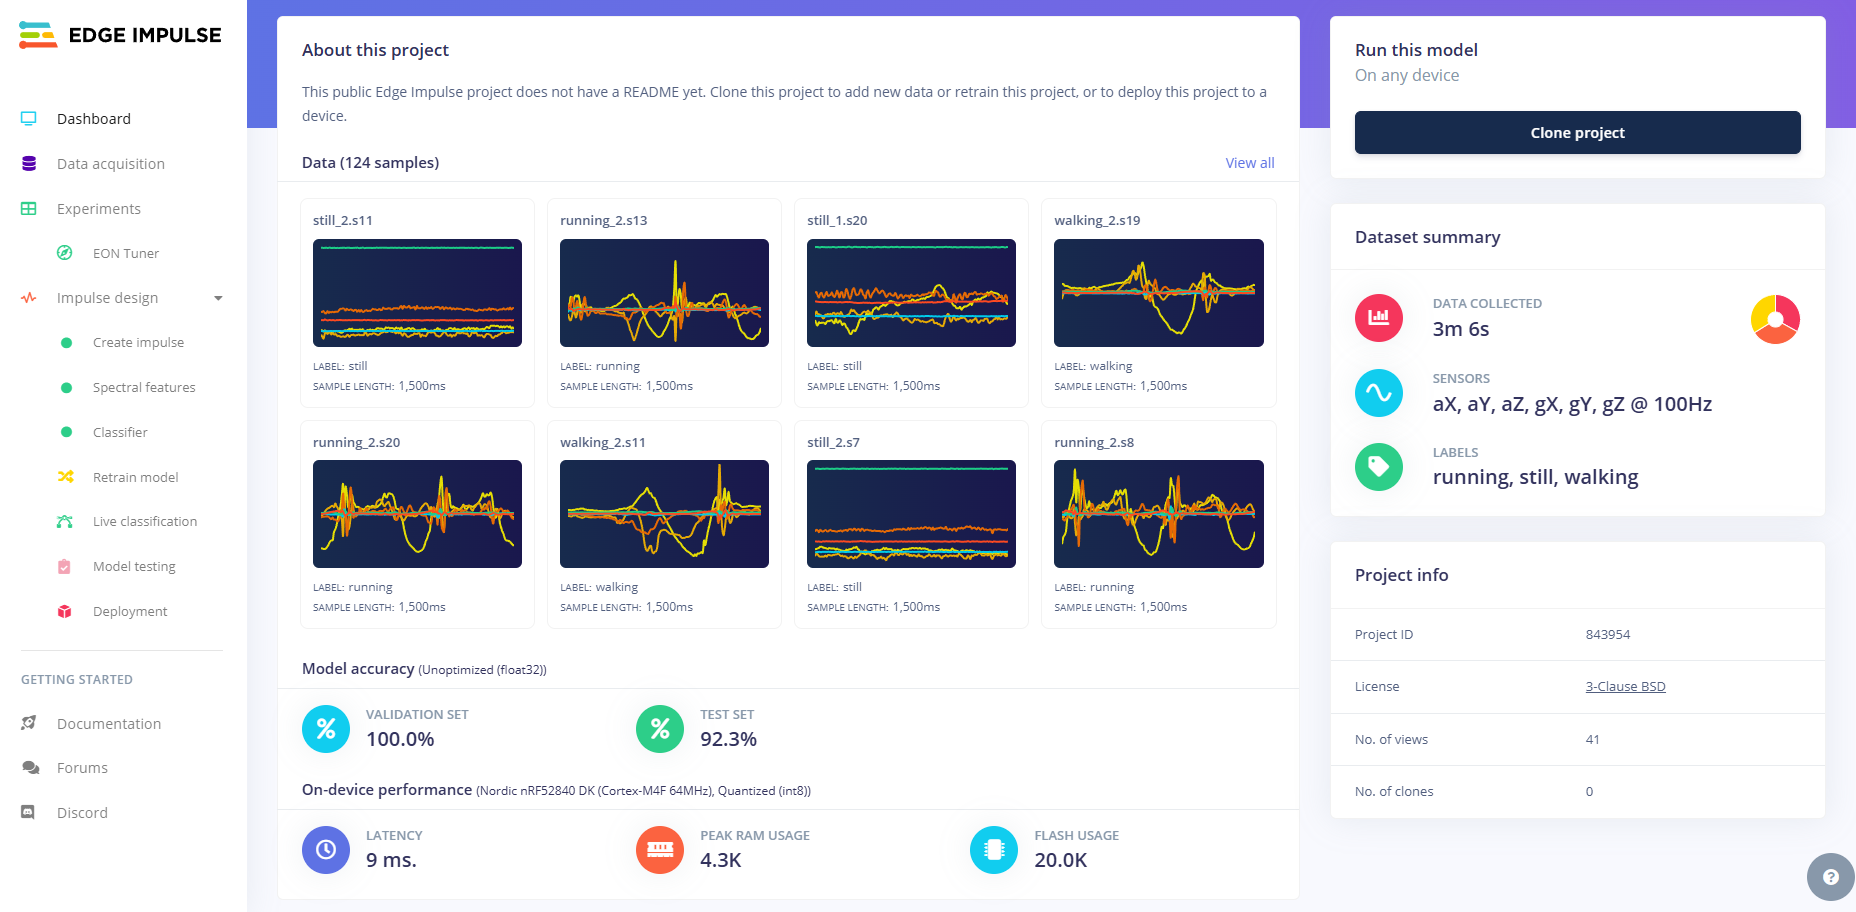
\includegraphics[width=0.85\textwidth]{figures/edge_impulse_interface.png}
\caption{Giao diện Edge Impulse (trang thiết kế Impulse): quy trình được định nghĩa bằng các block cố định, giới hạn khả năng tùy chỉnh tiền xử lý và thuật toán}
\label{fig:edge_impulse_ui}
\end{figure}

\subsection{Phân tích các nền tảng chính}

\paragraph{Edge Impulse \cite{web:Edge_Impulse}.} Nền tảng đám mây phổ biến nhất cho TinyML với EON Compiler tối ưu mã đầu ra và hỗ trợ 85+ mục tiêu vi điều khiển. Tuy nhiên, tiền xử lý bị cố định sau khi tải dữ liệu lên, không hỗ trợ phân đoạn tương tác; thuật toán chủ yếu giới hạn ở neural network; mã sinh ra là hộp đen không thể kiểm tra logic trích xuất đặc trưng; và dữ liệu phải lưu trên server của hãng, không phù hợp cho dữ liệu y tế nhạy cảm.

\paragraph{SensiML Analytics Toolkit \cite{web:SensiML}.} Hỗ trợ AutoML với hàng trăm đặc trưng ứng viên và Knowledge Packs cho MCU cụ thể. Hạn chế chính là chi phí rất cao, định dạng độc quyền, và lựa chọn đặc trưng theo kiểu hộp đen không giải thích được.

\paragraph{TensorFlow Lite Micro \cite{david2020tensorflow}.} Framework mã nguồn mở cung cấp runtime cho mạng nơ-ron lượng tử hóa trên MCU, tích hợp CMSIS-NN cho ARM và hỗ trợ INT8 quantization. Tuy nhiên, TFLite Micro chỉ hỗ trợ deep learning --- không triển khai được Random Forest hay SVM; không có công cụ tiền xử lý hay trích xuất đặc trưng; và interpreter runtime chiếm lượng flash đáng kể, đòi hỏi người dùng tự xây dựng toàn bộ pipeline từ đầu.

\paragraph{Teachable Machine (Google).} Giao diện no-code phù hợp cho tạo mẫu và giáo dục, nhưng thiếu trích xuất đặc trưng nâng cao, phân đoạn chuỗi thời gian, và chỉ xuất TensorFlow.js --- không chạy trên MCU.

\subsection{Tổng hợp khoảng trống}

Bảng~\ref{tab:platform_comparison} tổng hợp so sánh giữa các nền tảng và framework đề xuất.

\begin{table}[H]
\centering
\caption{So sánh các nền tảng Edge ML cho nhận dạng hoạt động}
\label{tab:platform_comparison}
\resizebox{\textwidth}{!}{%
\begin{tabular}{@{}p{4.0cm}p{3.2cm}p{3.2cm}p{3.2cm}p{4.4cm}@{}}
\toprule
\textbf{Tiêu chí} & \textbf{Edge Impulse} & \textbf{SensiML} & \textbf{TFLite Micro} & \textbf{Framework đề xuất} \\
\midrule
Chi phí & \$20--99/tháng & \$99--500/tháng & Miễn phí & Miễn phí (mã nguồn mở) \\
\midrule
Tiền xử lý tương tác & Hạn chế & Có (analytics) & Không & Có (kéo thả trên biểu đồ) \\
\midrule
Thuật toán & NN, transfer & RF, SVM, NN & Chỉ NN & RF, SVM, MLP, CNN \\
\midrule
Tạo mã & C++ (Arduino, ARM) & C (MCU cụ thể) & C++ (runtime) & C/C++/MicroPython đa đích \\
\midrule
Tối ưu hóa & Auto (EON) & AutoML & Lượng tử hóa & 4 chế độ rõ ràng \\
\midrule
Kiểm soát dữ liệu & Đám mây & Local/cloud & Local & Local hoàn toàn \\
\midrule
Xác minh tương đồng & Không minh bạch & Không & Không & Có (tự động) \\
\bottomrule
\end{tabular}%
}%
\end{table}

Điểm chung của các nền tảng hiện có: thiếu giao diện phân đoạn dữ liệu tương tác, bị giới hạn thuật toán hoặc chi phí cao, và sinh mã cho số ít nền tảng đích cố định. Đặc biệt, không nền tảng nào cung cấp cơ chế \textbf{xác minh tương đồng huấn luyện--triển khai} minh bạch. Khoảng trống này đặc biệt quan trọng trong bối cảnh nghiên cứu và giáo dục, nơi nhà nghiên cứu cần hiểu rõ pipeline, và các dự án nhỏ không có ngân sách cho giấy phép thương mại. \textbf{Luận văn này giải quyết khoảng trống đó} bằng một framework mã nguồn mở, minh bạch, hỗ trợ đa thuật toán và đa thiết bị.

\section{Phát biểu bài toán và mục tiêu nghiên cứu}
\label{sec:intro_problem}

\subsection{Phát biểu bài toán}

Từ các phân tích trên, bài toán nghiên cứu được phát biểu như sau:

\begin{quote}
\textit{Thiết kế và hiện thực một framework mã nguồn mở cho phép người dùng thực hiện toàn bộ quy trình HAR dựa trên cảm biến IMU --- từ thu thập dữ liệu, tiền xử lý tương tác, trích xuất đặc trưng, huấn luyện mô hình đa thuật toán, đến tự động sinh mã triển khai tối ưu cho nhiều họ vi điều khiển --- đồng thời đảm bảo tương đồng giữa kết quả huấn luyện và kết quả suy luận trên thiết bị biên.}
\end{quote}

Bài toán này đòi hỏi giải quyết đồng thời bốn thách thức: (1) hạ thấp rào cản kỹ thuật để người dùng không chuyên về nhúng vẫn triển khai được; (2) hỗ trợ nhiều thuật toán ML phù hợp cho tập dữ liệu nhỏ đến lớn; (3) sinh mã cho hệ sinh thái thiết bị phân mảnh; và (4) đảm bảo tính minh bạch và khả năng xác minh mã đã sinh.

\subsection{Mục tiêu nghiên cứu}

\begin{enumerate}
\item \textbf{Giao diện tiền xử lý tương tác}: Phát triển cơ chế phân đoạn và gán nhãn dữ liệu cảm biến trực tiếp trên biểu đồ tín hiệu bằng kéo thả, giảm thời gian chuẩn bị dữ liệu so với viết mã thủ công.

\item \textbf{Hỗ trợ đa thuật toán với giao diện thống nhất}: Tích hợp Random Forest, SVM, MLP, CNN với giao diện huấn luyện chung, cho phép so sánh và chọn mô hình phù hợp với từng ràng buộc phần cứng.

\item \textbf{Kiến trúc sinh mã đa đích}: Thiết kế hệ thống sinh mã phân lớp ánh xạ cùng một mô hình sang nhiều họ thiết bị (Arduino, ARM Cortex-M, ESP-IDF, Zephyr, MicroPython) với bốn chế độ tối ưu hóa (accuracy, speed, power, balanced).

\item \textbf{Đảm bảo tương đồng huấn luyện--triển khai}: Xây dựng cơ chế xác minh mã C++ sinh ra tái tạo chính xác công thức trích xuất đặc trưng, tham số chuẩn hóa, thứ tự đặc trưng và trọng số mô hình, đảm bảo nhất quán kết quả suy luận giữa Python và MCU.

\item \textbf{Xác thực trên phần cứng thực}: Đánh giá framework trên thiết bị ARM Cortex-M4F với dữ liệu HAR thực tế, đo thời gian suy luận, mức sử dụng bộ nhớ, và so sánh trực tiếp với nền tảng thương mại Edge Impulse.
\end{enumerate}

\subsection{Đóng góp chính}

Nghiên cứu này đóng góp vào lĩnh vực Edge ML và nhận dạng hoạt động qua các điểm mới sau:

\begin{enumerate}
    \item \textbf{Framework tích hợp toàn diện}: Lần đầu tiên kết hợp tiền xử lý tương tác (kéo thả trên biểu đồ), trích xuất đặc trưng minh bạch, huấn luyện đa thuật toán, và sinh mã đa đích trong cùng một hệ thống mã nguồn mở.
    
    \item \textbf{Cơ chế xác minh tương đồng huấn luyện--triển khai}: Quy trình kiểm tra 12 điểm đảm bảo mã C++ sinh ra tái tạo chính xác kết quả Python --- giải quyết vấn đề training--deployment gap mà các nền tảng hiện có bỏ qua.
    
    \item \textbf{Kiến trúc sinh mã đa chiều}: Mô hình Factory Pattern ánh xạ ba trục (loại mô hình × nền tảng đích × backend triển khai), cho phép một mô hình đã huấn luyện xuất đồng thời sang nhiều họ thiết bị mà không cần huấn luyện lại.
    
    \item \textbf{Phát hiện kỹ thuật mới}: Tài liệu hóa các lỗi tương đồng chưa được báo cáo trong tài liệu (zero-padding artifact, sai lệch population vs sample std trong kurtosis, feature order mismatch) --- kiến thức có giá trị cho cộng đồng TinyML.
    
    \item \textbf{Kết quả thực nghiệm}: Đạt 97--99\% trên bài toán 5 lớp, vượt trội Edge Impulse trên cùng tập dữ liệu (F1=1,00 vs 0,96), với mức sử dụng flash nhỏ hơn đáng kể (18--23\% vs 51\%) và thời gian suy luận 20~ms.
\end{enumerate}

Hình~\ref{fig:workflow} tổng hợp quy trình làm việc hoàn chỉnh mà framework cung cấp.

\begin{figure}[H]
\centering
\resizebox{\linewidth}{!}{%
\begin{tikzpicture}[
    node distance=0.55cm,
    stepbox/.style={
        rectangle, rounded corners=5pt,
        minimum width=2.6cm, minimum height=2.0cm,
        text width=2.5cm, align=center,
        draw=blue!45!black, fill=blue!6,
        line width=0.9pt, font=\small,
    },
    arr/.style={
        -{Stealth[length=7pt, width=5pt]},
        line width=2pt, color=black!35,
    },
    badge/.style={
        circle, fill=blue!65!black,
        minimum size=20pt, inner sep=0pt,
        font=\small\bfseries, text=white,
    },
    phaselbl/.style={
        font=\small\bfseries, text=black!65,
    },
    timelbl/.style={
        font=\scriptsize\itshape, text=black!45,
    },
]
    % --- Step boxes ---
    \node[stepbox] (s1) {\textbf{Dữ liệu}\\[4pt]\scriptsize Tải file CSV};
    \node[stepbox, right=of s1] (s2) {\textbf{Tiền xử lý}\\[4pt]\scriptsize Lọc \& phân đoạn};
    \node[stepbox, right=of s2] (s3) {\textbf{Đặc trưng}\\[4pt]\scriptsize Cửa sổ kéo thả};
    \node[stepbox, right=of s3] (s4) {\textbf{Huấn luyện}\\[4pt]\scriptsize RF / SVM / NN};
    \node[stepbox, right=of s4] (s5) {\textbf{Tạo mã}\\[4pt]\scriptsize C++ / Python};
    \node[stepbox, right=of s5] (s6) {\textbf{Thiết bị}\\[4pt]\scriptsize Triển khai biên};

    % --- Phase grouping backgrounds ---
    \begin{scope}[on background layer]
        \node[rectangle, rounded corners=8pt,
              fill=blue!10, draw=blue!30!black,
              inner sep=8pt, line width=0.8pt,
              fit=(s1)(s2)] (ph1) {};
        \node[rectangle, rounded corners=8pt,
              fill=teal!10, draw=teal!30!black,
              inner sep=8pt, line width=0.8pt,
              fit=(s3)(s4)] (ph2) {};
        \node[rectangle, rounded corners=8pt,
              fill=orange!10, draw=orange!30!black,
              inner sep=8pt, line width=0.8pt,
              fit=(s5)(s6)] (ph3) {};
    \end{scope}

    % --- Phase labels above groups ---
    \node[phaselbl, above=0.5cm of ph1] {Thu thập \& Xử lý};
    \node[phaselbl, above=0.5cm of ph2] {Xây dựng Mô hình};
    \node[phaselbl, above=0.5cm of ph3] {Triển khai Biên};

    % --- Arrows between steps ---
    \foreach \a/\b in {s1/s2, s2/s3, s3/s4, s4/s5, s5/s6}
        \draw[arr] (\a) -- (\b);

    % --- Step number badges centred on top border ---
    \foreach \n/\i in {s1/1, s2/2, s3/3, s4/4, s5/5, s6/6}
        \node[badge] at (\n.north) {\i};

    % --- Time labels below ---
    \node[timelbl, below=0.3cm of s1] {$\sim$5 phút};
    \node[timelbl, below=0.3cm of s2] {$\sim$10 phút};
    \node[timelbl, below=0.3cm of s3] {$\sim$2 phút};
    \node[timelbl, below=0.3cm of s4] {5--30 phút};
    \node[timelbl, below=0.3cm of s5] {$\sim$1 phút};
    \node[timelbl, below=0.3cm of s6] {$\sim$5 phút};
\end{tikzpicture}%
}
\caption{Quy trình làm việc từ dữ liệu thô đến triển khai biên (tổng ước tính 30--60 phút)}
\label{fig:workflow}
\end{figure}

\section{Phạm vi nghiên cứu}

Nghiên cứu tập trung vào HAR dựa trên IMU 6 trục (gia tốc kế + con quay hồi chuyển), sử dụng các thuật toán học máy có giám sát. Đánh giá phần cứng định lượng tập trung trên nền tảng tham chiếu Seeed XIAO nRF52840 (ARM Cortex-M4F, 64~MHz, 256~KB RAM); các nền tảng đích còn lại (ESP-IDF, Zephyr, MicroPython) được phân tích ở mức sinh mã và khả năng biên dịch.

Nghiên cứu không bao gồm: hợp nhất cảm biến đa phương thức (camera, âm thanh); nhập mô hình từ framework bên ngoài (TensorFlow SavedModel, ONNX); cập nhật mô hình trên thiết bị (on-device learning); và ứng dụng y tế đòi hỏi chứng nhận lâm sàng.

\section{Tổ chức luận văn}

Luận văn gồm sáu chương. \textbf{Chương~\ref{chap:relatedwork}} đánh giá các công trình liên quan về hệ thống HAR, framework học máy cho thiết bị biên, và các nền tảng triển khai edge ML hiện có. \textbf{Chương~\ref{chap:methodology}} trình bày phương pháp luận: quy trình tiền xử lý tín hiệu, các phương pháp trích xuất đặc trưng (miền thời gian, miền tần số, bất biến hướng), huấn luyện đa thuật toán, và chiến lược sinh mã đảm bảo tương đồng huấn luyện--triển khai. \textbf{Chương~\ref{chap:design_implementation}} mô tả thiết kế và hiện thực hệ thống, bao gồm kiến trúc phần mềm, giao diện người dùng và chi tiết triển khai các module. \textbf{Chương~\ref{chap:results}} báo cáo kết quả thực nghiệm: hiệu suất phân loại của năm thuật toán trên bài toán 3 và 5 lớp, đặc điểm triển khai trên thiết bị thực (thời gian suy luận, mức sử dụng bộ nhớ), và so sánh trực tiếp với Edge Impulse. \textbf{Chương~\ref{chap:discussion_conclusion}} trình bày kết luận, thảo luận các phát hiện chính, hạn chế và hướng phát triển tương lai.

\chapter{Các nghiên cứu liên quan}
\label{chap:relatedwork}

\section{Tổng quan}
Chương này trình bày các nghiên cứu liên quan trên các lĩnh vực chính: ứng dụng của theo dõi chuyển động, cảm biến quán tính cho HAR, các kiến trúc AI phù hợp, phương pháp tiền xử lý và trích xuất đặc trưng, kỹ thuật tối ưu hóa triển khai biên, và các khoảng trống nghiên cứu cần giải quyết.

\section{Các lĩnh vực ứng dụng của theo dõi chuyển động}
Theo dõi chuyển động con người là công nghệ nền tảng trong nhiều lĩnh vực. Trong y tế, cảm biến đeo cho phép phân tích dáng đi, phát hiện té ngã (độ nhạy 95--98\% \cite{wan2021deep_har_review}), và giám sát phục hồi chức năng \cite{article:human_motion_tracking_survey}. Thể thao tận dụng dữ liệu quán tính và sinh cơ học để tối ưu hiệu suất và phòng ngừa chấn thương. VR/AR phụ thuộc vào theo dõi khung xương chính xác cho trải nghiệm nhập vai. Ứng dụng công nghiệp gồm giám sát an toàn lao động, đạt 94,3\% trong phát hiện tư thế nguy hiểm tại công trường \cite{wang2023har_industrial}. Nhu cầu đa dạng này tạo động lực cho các framework theo dõi chuyển động hiệu quả, có khả năng suy luận biên thời gian thực với độ chính xác 90\%+.

\section{Theo dõi chuyển động dựa trên cảm biến}
Đơn vị đo lường quán tính (IMU)---kết hợp gia tốc kế và con quay hồi chuyển---được sử dụng rộng rãi trong theo dõi chuyển động nhờ tiêu thụ điện năng thấp (2--10~mA), chi phí thấp (\$1--5/đơn vị) và phù hợp để triển khai trên thiết bị biên. Filippeschi và cộng sự \cite{filippeschi2017survey_imu} tổng hợp các thách thức chính: trôi cảm biến (0,1--1$^\circ$/s cho con quay hồi chuyển), lỗi tích lũy trong ước lượng hướng, và yêu cầu hiệu chuẩn. Phương pháp hợp nhất đa cảm biến (IMU + từ kế + cảm biến áp suất) cải thiện độ chính xác 2--5\% nhưng tăng độ phức tạp và chi phí năng lượng. Xia và cộng sự \cite{xia2020lstm_har} đã chứng minh hệ thống IMU đơn đạt 96,8\% trên bài toán HAR 12 lớp với kiến trúc LSTM-CNN, xác nhận tính khả thi của cách tiếp cận cảm biến đơn.

Các tập dữ liệu chuẩn UCI-HAR \cite{anguita2013har} và WISDM \cite{banos2014wisdm} đều sử dụng IMU sáu trục gắn trên cơ thể ở 50--100~Hz, xác lập cấu hình này làm thiết lập tham chiếu cho nghiên cứu HAR trên thiết bị đeo. Framework trong luận văn kế thừa cấu hình đó---thu thập dữ liệu gia tốc kế và con quay hồi chuyển ba trục ở 100~Hz---tập trung vào quy trình IMU đơn với khả năng mở rộng đa cảm biến.

\section{Theo dõi chuyển động dựa trên thị giác}
Các phương pháp thị giác máy tính sử dụng camera và ước lượng tư thế (MediaPipe \cite{web:Google_Mediapipe}, OpenPose) cho phép tái tạo toàn thân (17+ điểm khóa, 30 FPS) và được dùng trong hoạt hình, phân tích lâm sàng. Tuy nhiên, hệ thống dựa trên thị giác gặp các hạn chế: che khuất trong cảnh đông đúc, nhạy với điều kiện ánh sáng, lo ngại quyền riêng tư khi thu hình ảnh, và tiêu thụ điện năng cao (500--2000~mW so với 20--50~mW của IMU). Đối với giám sát liên tục trên thiết bị đeo, nơi ưu tiên tuổi thọ pin (ngày đến tuần), các giải pháp IMU thuần túy vẫn là lựa chọn phù hợp nhất. Do đó, luận văn này tập trung hoàn toàn vào cảm biến quán tính.

\section{AI trong theo dõi chuyển động}
Các mô hình AI chuyển đổi dữ liệu chuyển động thô thành các nhận dạng ngữ nghĩa---phân loại hoạt động, nhận dạng tư thế và dự báo quỹ đạo. Phương pháp học máy truyền thống gồm Support Vector Machines (SVM) \cite{cortes1995svm} và Random Forests \cite{breiman2001random} đạt 88--93\% trên các benchmark chuẩn (UCI-HAR, WISDM) với bộ nhớ thời gian chạy 50--200~KB, phù hợp thiết bị biên \cite{wang2024har_comparative}.

Các kiến trúc học sâu cải thiện hiệu suất: CNN đạt 92--95\% (trích xuất đặc trưng không gian từ cửa sổ cảm biến), RNN/LSTM đạt 94--97\% (nắm bắt phụ thuộc thời gian \cite{xia2020lstm_har}), và transformer đạt 96--98\% trên tập dữ liệu phức tạp \cite{singh2023har_transformers}. Tuy nhiên, mô hình học sâu đòi hỏi tập dữ liệu lớn hơn (10.000+ mẫu so với 1.000--5.000 cho ML cổ điển), bộ nhớ cao hơn (500~KB--2~MB) và chiến lược lượng tử hóa phức tạp hơn khi triển khai biên \cite{lin2022mcunet}.

Nghiên cứu so sánh \cite{wang2024har_comparative} cho thấy ML cổ điển đạt 90--93\% với kích thước nhỏ hơn 10$\times$ và suy luận nhanh hơn 5--20$\times$ (12--18~ms so với 60--120~ms) trên Cortex-M4. Framework đề xuất hỗ trợ cả hai chiến lược---mô hình cổ điển cho kịch bản giới hạn tài nguyên, mạng nơ-ron nhẹ cho ứng dụng ưu tiên độ chính xác---với các chế độ tối ưu hóa giúp cân nhắc đánh đổi một cách có căn cứ.

\section{Các framework và nền tảng hiện có}
Như đã tổng quan trong Chương~\ref{chap:introduction}, nhiều nền tảng đã xuất hiện phục vụ phát triển mô hình AI cho thiết bị biên. Về mặt kỹ thuật, các hạn chế chính bao gồm:
\begin{itemize}
    \item \textbf{Edge Impulse} \cite{web:Edge_Impulse}: Quy trình tự động hóa cao nhưng cố định cửa sổ tiền xử lý sau khi tải dữ liệu; tinh chỉnh đòi hỏi tải lại toàn bộ. Logic tiền xử lý không minh bạch.
    \item \textbf{SensiML} \cite{web:SensiML}: AutoML với 200+ đặc trưng ứng viên nhưng sử dụng định dạng độc quyền và lựa chọn đặc trưng kiểu hộp đen.
    \item \textbf{TensorFlow Lite Micro} \cite{david2020tensorflow}: Runtime hiệu quả cho mạng nơ-ron lượng tử hóa trên vi điều khiển, nhưng chỉ hỗ trợ mạng nơ-ron và yêu cầu thiết kế kiến trúc thủ công.
    \item \textbf{Teachable Machine} \cite{web:Google_TeachableMachine}: Giao diện không mã cho tạo mẫu nhanh, nhưng thiếu trích xuất đặc trưng nâng cao và tối ưu hóa theo phần cứng.
    \item \textbf{AutoML/NAS} \cite{cai2018proxylessnas}: Tìm kiến trúc tối ưu dưới ràng buộc tài nguyên, nhưng đòi hỏi tài nguyên tính toán lớn và thiếu minh bạch.
\end{itemize}
Framework đề xuất giải quyết các hạn chế này bằng cách cung cấp: (1) tiền xử lý tương tác với phân đoạn kéo thả, (2) trích xuất đặc trưng minh bạch với kiểm tra từng đặc trưng, (3) tối ưu hóa đa mục tiêu theo ràng buộc phần cứng, và (4) mã nguồn mở không rào cản chi phí.

\section{Tiền xử lý dữ liệu và tạo cửa sổ}
Chất lượng nhận dạng hoạt động phụ thuộc nhiều vào chiến lược phân đoạn và tạo cửa sổ. Banos và cộng sự \cite{banos2014wisdm} đánh giá ảnh hưởng của kích thước cửa sổ: 1~giây đạt 89,3\%, 2,5~giây đạt 92,1\%, 5~giây đạt 93,4\% nhưng giảm khả năng phản hồi. Chồng lấp 50\% cải thiện 2--4\% so với cửa sổ không chồng lấp \cite{wan2021deep_har_review} với chi phí tính toán gấp đôi.

Lựa chọn bộ lọc ảnh hưởng đáng kể đến giảm nhiễu: bộ lọc thông thấp Butterworth (cutoff 20~Hz) bảo tồn đặc tính chuyển động trong khi làm suy giảm nhiễu cảm biến, cải thiện 3--7\% \cite{filippeschi2017survey_imu}. Tuy nhiên, quy trình tiền xử lý thông thường đòi hỏi sửa mã thủ công để điều chỉnh tham số lọc---các nhà phát triển thường dành 40--60\% thời gian dự án cho bước này \cite{merenda2020edge}. Nghiên cứu về học máy tương tác \cite{amershi2014power} chỉ ra rằng giao diện trực quan giảm 35\% thời gian lặp lại và 28\% lỗi so với quy trình dựa trên mã. Framework đề xuất áp dụng nguyên tắc này: cho phép căn chỉnh trực quan tín hiệu thô và đã xử lý, điều chỉnh cửa sổ tương tác với phản hồi tức thì, và gán nhãn nhanh.

\section{Trích xuất và biểu diễn đặc trưng}
Đặc trưng thủ công miền thời gian (trung bình, phương sai, RMS, độ lệch, độ nhọn, tỷ lệ qua không) và miền tần số (năng lượng phổ, tần số thống trị, entropy phổ) vẫn hiệu quả cho ML cổ điển khi được trích xuất có hệ thống \cite{oppenheim1999discrete}. Bộ đặc trưng điển hình gồm 60--150 đặc trưng mỗi cửa sổ \cite{wang2024har_comparative}. Lựa chọn đặc trưng (thông tin hỗ tương, kiểm định F ANOVA, loại bỏ đệ quy) có thể giảm 30--50\% chiều với mất độ chính xác dưới 2\%, đồng thời cải thiện tốc độ suy luận 15--30\% trên vi điều khiển \cite{banos2014wisdm}.

Đặc trưng miền tần số đặt ra thách thức triển khai: FFT trên hệ thống nhúng không có bộ tăng tốc phần cứng đòi hỏi O(N log N) phép toán dấu phẩy động, tiêu thụ 50--150~ms mỗi cửa sổ trên Cortex-M4 64~MHz \cite{banbury2021mlperf}. Các giải pháp nhẹ bao gồm đếm qua không, đỉnh tự tương quan, hoặc thư viện FFT tối ưu (ARM CMSIS-DSP). Quan trọng hơn, tính tương đồng đặc trưng giữa huấn luyện (Python NumPy FFT) và triển khai (C++ FFT điểm cố định) cần được xác minh cẩn thận.

Mặc dù mạng sâu end-to-end có thể học đặc trưng ngầm định, trích xuất đặc trưng tường minh cải thiện khả năng diễn giải và minh bạch triển khai---đặc biệt quan trọng trong các lĩnh vực y tế hoặc an toàn. Framework kết hợp các mô-đun đặc trưng hoán đổi được, xác minh tính nhất quán huấn luyện-triển khai, và hỗ trợ chẩn đoán từng cửa sổ.

\section{Triển khai biên và tối ưu hóa}
Ràng buộc tài nguyên định hình các thách thức triển khai biên: RAM hạn chế (32--256~KB), flash (256~KB--1~MB), không có hoặc hạn chế FPU, và ngân sách điện năng 10--50~mW cho thiết bị đeo \cite{banbury2021mlperf, ray2023tinyml_survey}. Benchmark MLPerf Tiny \cite{banbury2021mlperf} thiết lập số liệu tham chiếu: Cortex-M4F 64~MHz đạt 10,3 suy luận/giây cho phát hiện từ khóa (mô hình 49~KB), 15,2 suy luận/giây cho phát hiện bất thường (mô hình 32~KB). Các chiến lược tối ưu hóa chính:
\begin{itemize}
    \item \textbf{Lượng tử hóa}: Float 32-bit sang số nguyên 8-bit giảm kích thước 4$\times$, tăng tốc suy luận 2--3$\times$ với suy giảm 0,5--2\% \cite{lin2022mcunet}.
    \item \textbf{Cắt tỉa}: Loại bỏ 40--70\% trọng số (theo độ lớn hoặc cấu trúc) cho tăng tốc 2--3$\times$ với mất dưới 1\% \cite{schmidhuber2015deep}.
    \item \textbf{Chưng cất kiến thức}: Mô hình nhỏ (10--20\% tham số) bắt chước mô hình lớn, đạt 85--95\% hiệu suất với kích thước nhỏ hơn 5--10$\times$ \cite{dutta2023tinyml_platforms}.
    \item \textbf{ML cổ điển}: Random Forests (độ sâu $\leq$10) và SVM (100--500 support vectors) đạt 88--93\% với 50--200~KB bộ nhớ, suy luận 12--25~ms \cite{wang2024har_comparative}.
\end{itemize}
Các khảo sát TinyML \cite{ray2023tinyml_survey, dutta2023tinyml_platforms} nhận diện ba mẫu triển khai: (1) ưu tiên độ trễ dùng ML cổ điển (5--20~ms), (2) ưu tiên độ chính xác dùng CNN/LSTM nhẹ (40--80~ms, cao hơn 1--2\%), (3) ưu tiên điện năng dùng lấy mẫu thưa và lượng tử hóa mạnh. Thành phần sinh mã của framework thực hiện xuất mã C/C++ theo nền tảng với chuyển đổi tham số phù hợp ràng buộc, và các chế độ tối ưu hóa đa mục tiêu cho phép lựa chọn có căn cứ giữa độ chính xác, tốc độ và tiêu thụ điện năng.

\section{Các khoảng trống trong công trình hiện có}
Mặc dù hệ sinh thái công cụ edge AI đã khá hoàn thiện, một số khoảng trống quan trọng vẫn tồn tại:
\begin{enumerate}
    \item \textbf{Tiền xử lý tương tác hạn chế}: Ít hệ thống cho phép kiểm tra trực quan tín hiệu thô so với đã lọc và tinh chỉnh phân đoạn thủ công trong cùng môi trường.
    \item \textbf{Thiếu minh bạch trong trích xuất đặc trưng}: Các công cụ tạo đặc trưng tự động che giấu bước dẫn xuất, cản trở mục đích giáo dục và tái tạo nghiên cứu.
    \item \textbf{Sinh mã triển khai thiếu linh hoạt}: Mã đầu ra thường là khối nguyên, khó tùy chỉnh hoặc thích ứng theo phần cứng cụ thể.
    \item \textbf{Đánh đổi giữa dễ sử dụng và kiểm soát}: Các nền tảng hiện tại thường thiên về một cực---dễ dùng như Teachable Machine, hoặc linh hoạt cao như TensorFlow---ít nền tảng cân bằng được cả hai cho quy trình xử lý dữ liệu cảm biến chuyển động.
\end{enumerate}
Framework đề xuất giải quyết các khoảng trống này bằng cách thống nhất tiền xử lý tương tác, trích xuất đặc trưng minh bạch, huấn luyện modular và sinh mã tối ưu hóa dưới một kiến trúc mở rộng.

\section{Tóm tắt}
Các nghiên cứu và nền tảng công nghiệp trước đây cung cấp nền tảng vững chắc cho theo dõi chuyển động, nhưng chưa có nền tảng nào cung cấp quy trình tích hợp, minh bạch và thân thiện với người dùng, được tối ưu hóa cho triển khai biên dựa trên IMU với khả năng phân đoạn dữ liệu tương tác. Công trình này xây dựng trên các thuật toán và thực hành edge ML đã được thiết lập, đồng thời đóng góp phương pháp mới giúp phổ cập quy trình phát triển, tăng tốc lặp lại và cải thiện tính sẵn sàng triển khai cho các ứng dụng theo dõi chuyển động thực tế.

\chapter{Phương pháp luận}
\label{chap:methodology}

Chương này trình bày cơ sở lý thuyết và phương pháp cho từng giai đoạn trong pipeline: lý do chọn cảm biến IMU, các kỹ thuật lọc và phân đoạn tín hiệu, chiến lược trích xuất đặc trưng, thuật toán học máy, và hệ thống tạo mã triển khai. Kiến trúc hệ thống tổng thể và các quyết định thiết kế phần mềm được trình bày trong Chương~\ref{chap:design_implementation}.

\section{Dữ liệu cảm biến quán tính cho nhận dạng hoạt động}
\label{sec:imu_data_rationale}

Cảm biến gia tốc kế đo gia tốc tuyến tính trên ba trục (bao gồm thành phần trọng lực), phản ánh biên độ và tính tuần hoàn của chuyển động. Tuy nhiên, khi thiết bị xoay, vectơ trọng trường chiếu lên các trục thay đổi, gây nhập nhằng giữa chuyển động tịnh tiến và thay đổi định hướng. Cảm biến con quay hồi chuyển đo vận tốc góc (°/s), không bị ảnh hưởng bởi trọng trường và nắm bắt chính xác động học xoay---giúp phân biệt các cặp hoạt động khó như leo/xuống cầu thang hay đi bộ/giậm chân tại chỗ. Tổ hợp sáu trục (3 gia tốc kế + 3 con quay hồi chuyển) cung cấp biểu diễn động học đầy đủ \cite{filippeschi2017survey_imu}, và đây là cấu hình chuẩn trong các tập dữ liệu HAR như UCI-HAR \cite{anguita2013har} và PAMAP2 \cite{reiss2012pamap2}.

Framework không áp đặt tần số lấy mẫu cố định, nhưng có một ràng buộc bắt buộc: \textbf{tần số lấy mẫu phải nhất quán giữa giai đoạn huấn luyện và suy luận triển khai}. Các đặc trưng thống kê được tính theo \textit{số mẫu} trong cửa sổ, không theo thời gian tuyệt đối---nếu tần số thay đổi, cùng một cửa sổ 150 mẫu sẽ đại diện cho khoảng thời gian khác nhau, làm lệch toàn bộ phân phối đặc trưng. Để đảm bảo tính nhất quán, framework nhúng tần số lấy mẫu đã chọn dưới dạng hằng số biên dịch vào mã triển khai. Đối với HAR, dải tần phổ hoạt động phổ biến nằm trong 1--20~Hz \cite{whittle2014gait}, nên tần số lấy mẫu 50--100~Hz là phù hợp.

\section{Quy trình tiền xử lý tương tác}

\subsection{Tải lên và trực quan hóa dữ liệu}
Người dùng tải lên các tập dữ liệu CSV chứa các phép đo IMU, tổ chức theo hoạt động (mỗi tệp tương ứng với một lớp). Framework tự động phát hiện tên cột cảm biến, tần số lấy mẫu và hiển thị biểu đồ đồng bộ của tín hiệu thô trên tất cả các trục, cho phép kiểm tra trực quan chất lượng dữ liệu trước khi tiền xử lý (xem giao diện tại Hình~\ref{fig:ui_data_upload}, Chương~\ref{chap:design_implementation}).

\subsection{Các phương pháp lọc và làm sạch tín hiệu}
\label{sec:signal_filtering}

Dữ liệu IMU thô chứa nhiễu cảm biến, nhiễu điện từ và các xung bất thường cần được loại bỏ trước khi trích xuất đặc trưng. Framework cung cấp năm phương pháp lọc, mỗi phương pháp có đặc tính khác nhau về mức độ làm mịn, tính nhân quả và---quan trọng nhất cho triển khai nhúng---\textit{tính tương đồng huấn luyện-triển khai} (training-deployment parity). Người dùng chọn phương pháp phù hợp qua giao diện tương tác; kết quả lọc được trực quan hóa cùng tín hiệu gốc để đánh giá hiệu quả trước khi phân đoạn.

\subsubsection{Loại bỏ ngoại lệ (outlier removal)}
Xác định và loại bỏ các mẫu có giá trị vượt quá ngưỡng $k\sigma$ so với trung bình cục bộ (mặc định $k=3$). Đây là bước làm sạch thô, xử lý các xung nhiễu điện từ hoặc bất thường phần cứng (spike artifacts) tạo ra giá trị nằm ngoài phạm vi vật lý hợp lệ của cảm biến. Phương pháp này không thay đổi hình dạng tín hiệu mà chỉ loại bỏ các điểm dữ liệu cô lập rõ ràng sai, nên không có vấn đề parity---nó chỉ áp dụng một lần trên tập dữ liệu huấn luyện (offline) và không cần triển khai trên thiết bị.

\subsubsection{Bộ lọc Butterworth low-pass}
Bộ lọc IIR Butterworth bậc $n$ với tần số cắt $f_c$ có đáp ứng biên độ cực đại phẳng (maximally flat):
$$|H(f)|^2 = \frac{1}{1 + (f/f_c)^{2n}}$$
Để tránh lệch pha, kỹ thuật lọc hai chiều (forward-backward filtfilt) được sử dụng, cho đáp ứng $|H_{\text{eff}}|^2 = |H|^4$ với pha bằng không. Cấu hình mặc định: bậc 2, tần số cắt 5~Hz.

\textbf{Parity triển khai}: Vì HAR đệm toàn bộ cửa sổ $W$ mẫu trước khi xử lý, thiết bị thực hiện cùng thao tác lọc hai chiều trên bộ đệm. Các hệ số được tính trước tại thời điểm sinh mã và nhúng dưới dạng hằng số.

\subsubsection{Bộ lọc Savitzky-Golay}
Bộ lọc Savitzky-Golay \cite{savitzky1964smoothing} khớp đa thức bậc $d$ lên cửa sổ $2m+1$ mẫu bằng bình phương tối thiểu, cho kết quả tương đương tích chập FIR với các hệ số $c_j$ được tính từ ma trận Vandermonde. So với trung bình động, phương pháp bảo tồn tốt hơn các đỉnh tín hiệu. Cấu hình mặc định: $m=2$ (cửa sổ 5 mẫu), $d=2$.

\textbf{Parity triển khai}: Các hệ số $c_j$ được tính trước và nhúng vào mã C++ dưới dạng mảng hằng số; tích chập áp dụng trên bộ đệm cửa sổ với mở rộng biên bằng lặp giá trị biên.

\subsubsection{Bộ lọc FFT low-pass (miền tần số)}
Lọc trong miền tần số thực hiện ba bước: DFT, triệt tiêu các bin tần số cao ($k > k_c = \lfloor f_c N / f_s \rfloor$), rồi IDFT. Đặc điểm: đáp ứng tần số lý tưởng (brick-wall) và không méo pha. Chi phí bộ nhớ $\mathcal{O}(N)$.

\textbf{Parity triển khai}: Thiết bị thực thi cùng ba bước DFT~$\to$~masking~$\to$~IDFT trên bộ đệm cửa sổ với cùng $k_c$, dùng số dấu phẩy động 32-bit nhất quán.

\subsubsection{Bộ lọc Kalman (constant-velocity)}
\label{sec:kalman_filter}

Bộ lọc Kalman constant-velocity 1D \cite{kalman1960new} áp dụng cho mỗi kênh cảm biến IMU được đề xuất như giải pháp lọc có \textit{khoảng cách parity bằng không}. Bộ lọc Kalman hoạt động hoàn toàn theo chiều thuận (forward-only, causal) trong cả hai môi trường: Python huấn luyện \textit{và} C++ triển khai---loại bỏ lớp lỗi mà tất cả bốn phương pháp trên gặp phải.

\textbf{Mô hình toán học.} Mỗi kênh cảm biến được mô hình hóa bằng trạng thái gồm vị trí (giá trị cảm biến) và vận tốc:
$$\mathbf{x}_k = \begin{bmatrix} p_k \\ v_k \end{bmatrix}, \quad
F = \begin{bmatrix} 1 & \Delta t \\ 0 & 1 \end{bmatrix}, \quad
H = \begin{bmatrix} 1 & 0 \end{bmatrix}$$

Ma trận hiệp phương sai nhiễu quá trình:
$$Q = q \begin{bmatrix} \frac{\Delta t^3}{3} & \frac{\Delta t^2}{2} \\ \frac{\Delta t^2}{2} & \Delta t \end{bmatrix}$$

Nhiễu đo: $R = r$ (scalar). Hai tham số điều chỉnh được: $q$ (process noise, mặc định $10^{-3}$---nhỏ hơn = mượt hơn) và $r$ (measurement noise, mặc định $10^{-1}$---lớn hơn = mượt hơn). Kalman gain $K_k$ tự động thích ứng theo tín hiệu: tăng khi tín hiệu biến đổi nhanh (bám sát), giảm khi tín hiệu ổn định (lọc mạnh hơn).

\subsubsection{So sánh tổng hợp các phương pháp lọc}

Bảng~\ref{tab:filter_parity_comparison} tổng hợp năm phương pháp theo tiêu chí quan trọng nhất cho hệ thống triển khai nhúng:

\begin{table}[H]
    \centering
    \caption{So sánh các phương pháp lọc theo tính tương đồng huấn luyện-triển khai}
    \label{tab:filter_parity_comparison}
    \small
    \begin{tabular}{@{}p{2.8cm}ccp{4.2cm}@{}}
        \toprule
        Phương pháp & Causal & Parity & Ghi chú triển khai \\
        \midrule
        Loại bỏ ngoại lệ & --- & \checkmark & Chỉ offline (không cần trên thiết bị) \\
        Butterworth LP & Không$^\dag$ & \checkmark & Per-window two-pass filtfilt trên bộ đệm cửa sổ \\
        Savitzky-Golay & Không$^\dag$ & \checkmark & FIR convolution với hệ số tiền tính \\
        FFT low-pass & Không$^\dag$ & \checkmark & DFT trực tiếp trên bộ đệm cửa sổ \\
        \textbf{Kalman filter} & \textbf{Có} & \checkmark & Forward-only; hoạt động cả streaming lẫn windowed \\
        \bottomrule
    \end{tabular}
    \vspace{4pt}
    \begin{minipage}{\linewidth}
    \footnotesize
    $^\dag$Non-causal trong streaming; parity đạt được nhờ HAR đệm toàn bộ cửa sổ trước khi trích xuất đặc trưng, cho phép áp dụng bộ lọc hai chiều trên bộ đệm.
    \end{minipage}
\end{table}

Kết luận thiết kế: tất cả các phương pháp lọc đều đạt parity hoàn toàn khi suy luận HAR thực hiện theo lô cửa sổ, vì quy trình đã đệm toàn bộ $W$ mẫu trước khi trích xuất đặc trưng---ràng buộc non-causal chỉ áp dụng cho streaming theo từng mẫu. Kalman filter có lợi thế bổ sung: hoạt động được trong cả chế độ streaming lẫn lô, phù hợp cho hiển thị tín hiệu thời gian thực trong quá trình thu thập. Loại bỏ ngoại lệ không được nhân bản trên thiết bị vì cần thống kê toàn cục từ toàn bộ bản ghi, trong khi mỗi chu kỳ suy luận chỉ có một cửa sổ 1,5~giây.

\subsection{Phân đoạn và sinh cửa sổ huấn luyện}
\label{sec:windowing_generation}

Máy học trên tín hiệu liên tục đòi hỏi chuyển đổi chuỗi thời gian thành các vector có độ dài cố định. Framework thực hiện qua hai bước: người dùng xác định các đoạn tín hiệu sạch trên biểu đồ, và hệ thống tự động sinh cửa sổ huấn luyện bằng giải thuật cửa sổ trượt.

\subsubsection{Giải thuật cửa sổ trượt tự động}

Cho đoạn tín hiệu $N$ mẫu, kích thước cửa sổ $W$ và độ chồng lấp $o$~(\%), bước trượt $S = W \cdot (1 - o/100)$, số cửa sổ sinh được:
\begin{equation}
    n_w = \left\lfloor \frac{N - W}{S} \right\rfloor + 1
    \label{eq:sliding_window}
\end{equation}
Ví dụ: đoạn 5~giây (500 mẫu ở 100~Hz) với $W = 150$, $o = 50\%$ sinh ra 6 cửa sổ huấn luyện. Overlap 50\% tăng gấp đôi số mẫu từ cùng lượng dữ liệu thô, đồng thời giảm hiệu ứng biên---cùng một sự kiện chuyển động xuất hiện ở vị trí tương đối khác nhau trong các cửa sổ kế tiếp, giúp mô hình học đặc trưng bất biến vị trí. Overlap cao hơn ($>$75\%) tạo ra tương quan cao giữa các cửa sổ liên tiếp, tăng nguy cơ rò rỉ thông tin.

\subsubsection{Lựa chọn đoạn tương tác}

Giao diện kéo thả cho phép người dùng đánh dấu các vùng sạch trên biểu đồ tín hiệu, bỏ qua đoạn chuyển tiếp hoặc nhiễu. Nhiều đoạn trên cùng một tệp được hỗ trợ. Sau khi xác nhận, cửa sổ trượt chạy tự động trên từng đoạn theo Phương trình~\ref{eq:sliding_window}. Nhãn hoạt động kế thừa từ tệp nguồn nhưng có thể gán lại thủ công. Thiết kế này tách bạch hai quyết định: \textit{đâu là dữ liệu đáng tin cậy} (người dùng kiểm soát) và \textit{cách biến dữ liệu thành mẫu huấn luyện} (hệ thống tự động hóa), giảm đáng kể công sức thu thập trong khi bảo tồn kiểm soát chất lượng (xem Hình~\ref{fig:ui_preprocessing}, Chương~\ref{chap:design_implementation}).

\section{Trích xuất đặc trưng}
\label{sec:feature_extraction}

\subsection{Tham số cửa sổ và ràng buộc nhất quán}

Trích xuất đặc trưng thực hiện trên các cửa sổ được sinh theo Mục~\ref{sec:windowing_generation}: $W = 150$ mẫu (1,5 giây ở $f_s = 100$~Hz), bước trượt $S = 75$ (50\% chồng lấp). Ràng buộc cốt lõi: ($W$, $S$, $f_s$) phải đồng nhất giữa huấn luyện và suy luận---thay đổi $W$ sau huấn luyện làm lệch phân phối đặc trưng. Framework nhúng $W$ và $f_s$ dưới dạng hằng số trong mã sinh ra.

\subsection{Các loại trích xuất đặc trưng}
\label{sec:feature_modes}

Sáu loại trích xuất đặc trưng được thiết kế để đáp ứng các yêu cầu khác nhau về số chiều, khả năng triển khai nhúng và bất biến hướng. Bảng~\ref{tab:feature_modes} tóm tắt toàn diện.

\begin{table}[ht]
\centering
\caption{Sáu loại trích xuất đặc trưng: tín hiệu nguồn, cấu thành và đặc tính triển khai}
\label{tab:feature_modes}
\small
\resizebox{\textwidth}{!}{%
\begin{tabular}{@{}p{3.2cm}p{3.8cm}p{3.2cm}ccc@{}}
\toprule
\textbf{Loại} & \textbf{Tín hiệu nguồn} & \textbf{Đặc trưng tính} & \textbf{\#} & \textbf{Nhúng} & \textbf{OI\textsuperscript{*}} \\
\midrule
\texttt{oi\_time\_only}\textsuperscript{1}
  & acc\_mag, gyro\_mag, acc\_jerk\_mag
  & 15 thống kê thời gian / tín hiệu
  & 41 & \checkmark & \checkmark \\[3pt]
\texttt{orientation\_invariant}
  & Như trên + DFT(acc\_mag, gyro\_mag)
  & Như trên + 10 phổ / DFT
  & 63 & \checkmark & \checkmark \\[3pt]
\texttt{time\_domain}
  & aX, aY, aZ, gX, gY, gZ
  & 15 thống kê / trục
  & 90 & \checkmark & $\times$ \\[3pt]
\texttt{all}
  & aX, aY, aZ, gX, gY, gZ
  & 15 thời gian + 11 tần số / trục
  & 156 & $\times$ & $\times$ \\[3pt]
\texttt{frequency\_domain}
  & aX, aY, aZ, gX, gY, gZ
  & 11 đặc trưng phổ / trục
  & 66 & $\times$ & $\times$ \\[3pt]
\texttt{raw}
  & aX, aY, aZ, gX, gY, gZ
  & Giá trị cảm biến thô
  & 6 & \checkmark & $\times$ \\
\bottomrule
\end{tabular}%
}
\vspace{4pt}
\begin{minipage}{\linewidth}
\footnotesize
\textsuperscript{1}\texttt{oi\_time\_only} = \texttt{orientation\_invariant\_time\_only}.\\
\textsuperscript{*}OI = Orientation-Invariant (bất biến hướng).
Tín hiệu tổng hợp: $\text{acc\_mag} = \sqrt{a_X^2+a_Y^2+a_Z^2}$;
$\text{gyro\_mag} = \sqrt{g_X^2+g_Y^2+g_Z^2}$;
$\text{acc\_jerk\_mag} = \tfrac{d}{dt}\,\text{acc\_mag}$.
\end{minipage}
\end{table}

Hai loại \textbf{bất biến hướng} tính đặc trưng trên biên độ tổng hợp (vector magnitude)---đại lượng bất biến phép xoay---phù hợp khi thiết bị đeo không cố định. Loại \texttt{orientation\_invariant} (63 đặc trưng) là khuyến nghị mặc định: cân bằng giữa tính phong phú và triển khai nhúng, vì bộ sinh mã tạo DFT bằng tổng sin/cos trực tiếp không cần thư viện FFT.

Loại \texttt{time\_domain} (90 đặc trưng) áp dụng 15 thống kê lên từng trục riêng lẻ---mỗi đặc trưng là biểu thức dạng đóng xác định, không phụ thuộc trạng thái, đảm bảo bit-identical trên mọi nền tảng:
\begin{itemize}
    \item \textbf{Xu hướng trung tâm}: mean, median
    \item \textbf{Phân tán}: std, range, IQR
    \item \textbf{Cực trị}: min, max, Q1, Q3
    \item \textbf{Hình dạng}: skewness $\gamma = E[(X-\mu)^3]/\sigma^3$, kurtosis $\kappa = E[(X-\mu)^4]/\sigma^4 - 3$
    \item \textbf{Năng lượng}: RMS, signal energy
    \item \textbf{Xấp xỉ tần số}: zero-crossing rate, mean-crossing rate
\end{itemize}

Loại \texttt{all} và \texttt{frequency\_domain} bổ sung đặc trưng phổ mỗi trục nhưng \textbf{không hỗ trợ triển khai nhúng} vì nhạy với sai lệch số, tốn tài nguyên tính toán, và đặc trưng miền thời gian đã đủ hiệu quả trên các tập HAR chuẩn~\cite{banos2014wisdm}. Loại \texttt{raw} truyền trực tiếp giá trị cảm biến, dùng làm đầu vào CNN.

\subsection{Chiến lược đệm cửa sổ}
\label{sec:window_padding}

Các cửa sổ có thể ngắn hơn kích thước mục tiêu khi người dùng chọn đoạn ngắn hoặc cửa sổ cuối không đủ dài.

\textbf{Vấn đề với zero-padding}: Đặt giá trị cảm biến bằng 0 tạo ra magnitude gia tốc $||\mathbf{a}|| = 0$---vật lý bất khả thi vì gia tốc trọng trường luôn $\approx 9{,}81$ m/s². Điều này gây nhiễu nghiêm trọng cho phân phối đặc trưng (min, median, Q1 bị kéo về 0).

\textbf{Giải pháp}: Lặp giá trị cuối cùng đến kích thước mục tiêu: $\mathbf{W}' = [w_1, \ldots, w_k, \underbrace{w_k, \ldots, w_k}_{N-k}]$. Phương pháp bảo toàn tính thống kê tín hiệu và nhất quán với bộ đệm trên thiết bị biên (luôn chứa dữ liệu thực). Cửa sổ có ít hơn 30\% mẫu mục tiêu bị loại bỏ hoàn toàn.

\textit{Phát hiện thực nghiệm}: Zero-padding khiến mô hình luôn dự đoán sai lớp \textit{walking\_downstairs} bất kể hoạt động thực tế, do đặc trưng nằm ngoài phân phối huấn luyện (xem Mục~\ref{sec:training_deployment_parity}).

\subsection{Tăng cường dữ liệu cho huấn luyện}
\label{sec:data_augmentation}

Để cải thiện tính tổng quát hóa và giảm overfitting---đặc biệt với tập dữ liệu nhỏ từ thu thập đối tượng đơn---năm phương pháp tăng cường dữ liệu được áp dụng ở cấp cửa sổ (trước trích xuất đặc trưng) \cite{um2017data, iwana2021empirical}:

\begin{enumerate}
    \item \textbf{Jitter}: Nhiễu Gaussian $\mathcal{N}(0, \sigma^2)$ ($\sigma=0{,}05$), mô phỏng nhiễu cảm biến \cite{um2017data}
    \item \textbf{Scaling}: Nhân hệ số $s \sim \mathcal{N}(1, \sigma_s^2)$, mô phỏng biên độ chuyển động khác nhau
    \item \textbf{Rotation}: Ma trận xoay ngẫu nhiên ($\leq 15^{\circ}$), mô phỏng thay đổi vị trí cảm biến \cite{eyobu2018feature}
    \item \textbf{Time Warping}: Biến đổi phi tuyến trục thời gian qua nội suy spline, mô phỏng tốc độ thực hiện khác nhau \cite{le_guennec2016augmentation}
    \item \textbf{Permutation}: Hoán vị $k=4$ đoạn con, giúp mô hình học đặc trưng cục bộ thay vì phụ thuộc thứ tự toàn cục
\end{enumerate}

\subsubsection{Tăng cường nhận biết lớp}
\label{sec:class_aware_augmentation}

Áp dụng biến đổi mạnh lên hoạt động tĩnh (still, standing, sitting) tạo dao động nhỏ giống hoạt động cường độ thấp, gây nhầm lẫn lớp. Framework giải quyết bằng chiến lược phân biệt:
\begin{itemize}
    \item \textbf{Hoạt động động}: Áp dụng đầy đủ cả năm phương pháp ($\sigma_{\text{jitter}} = 0{,}05$)
    \item \textbf{Hoạt động tĩnh}: Chỉ micro-jitter ($\sigma = 0{,}01$)---đủ tạo đa dạng mà không phá vỡ đặc tính ``gần bất động''
\end{itemize}
Phân loại tĩnh/động dựa trên ngưỡng biên độ dao động và có thể do người dùng chỉ định thủ công. Chiến lược tuân thủ nguyên tắc rằng tăng cường phải bảo toàn các đặc tính phân biệt của mỗi lớp \cite{buda2018systematic}.

\subsection{Ngưỡng tin cậy cho từ chối hoạt động không xác định}
\label{sec:confidence_threshold}

Trong triển khai thực tế, thiết bị có thể ghi nhận chuyển động không thuộc lớp nào đã huấn luyện. Ngưỡng tin cậy $\tau$ (mặc định 0,6) được tích hợp vào mã suy luận: nếu $\max_c P(y=c|\mathbf{x}) < \tau$, dự đoán trả về ``unknown'' thay vì ép buộc một nhãn:
\begin{equation}
    \hat{y} = \begin{cases}
        \arg\max_c P(y=c|\mathbf{x}) & \text{nếu } \max_c P(y=c|\mathbf{x}) \geq \tau \\
        \text{unknown} & \text{ngược lại}
    \end{cases}
\end{equation}

Xác suất từng lớp được tính theo cơ chế có sẵn: softmax cho NN/CNN, tỷ lệ bỏ phiếu cho RF, softmax trên điểm quyết định OvR cho SVM. Giá trị $\tau = 0{,}6$ yêu cầu tin cậy gấp 3 lần xác suất ngẫu nhiên (bài toán 5 lớp: 20\%). So với Edge Impulse (cần huấn luyện khối anomaly detection riêng), cách tiếp cận này không tốn thêm bộ nhớ hay dữ liệu bổ sung.

\section{Huấn luyện mô hình học máy}

\subsection{Các thuật toán học máy áp dụng}
Bốn nhóm thuật toán học máy dưới đây đã được chứng minh hiệu quả trong nhận dạng hoạt động và phù hợp cho triển khai biên, với các đánh đổi khác nhau giữa độ chính xác, yêu cầu dữ liệu và chi phí tài nguyên:

\paragraph{Random Forest (RF)}
Phương pháp ensemble kết hợp nhiều cây quyết định với bagging và ngẫu nhiên hóa đặc trưng \cite{breiman2001random}. Cấu hình điển hình cho bài toán HAR:
\begin{itemize}
    \item Số cây: 50--200 (tham chiếu: 100 cây), độ sâu tối đa 10--30
    \item Cân bằng lớp: \texttt{class\_weight='balanced'} tự động trọng số mẫu tỷ lệ nghịch với tần suất lớp
    \item Tiêu chí phân nhánh: Độ bất thuần Gini hoặc entropy thông tin
\end{itemize}
RF đặc biệt phù hợp cho HAR vì không yêu cầu chuẩn hóa đặc trưng; chịu đựng tốt với đặc trưng không liên quan (mỗi lần phân nhánh chỉ xét $\sqrt{D}$ đặc trưng ngẫu nhiên); kết quả giải thích được qua độ quan trọng đặc trưng; ổn định với nhiễu nhờ cơ chế bỏ phiếu đa số.

\paragraph{Support Vector Machine (SVM)}
Bộ phân loại phân biệt tìm siêu phẳng tối đa hóa biên phân tách giữa các lớp. Cấu hình điển hình:
\begin{itemize}
    \item Kernel: Radial Basis Function (RBF), phù hợp cho dữ liệu phi tuyến; tham số gamma kiểm soát bán kính ảnh hưởng của từng điểm huấn luyện
    \item Chiến lược đa lớp: One-vs-One (OvO) hoặc One-vs-Rest (OvR)
    \item Cân bằng lớp: \texttt{class\_weight='balanced'}
    \item Chính quy hóa: Tham số $C$ kiểm soát đánh đổi biên rộng---vi phạm biên ($C \in \{0{,}1;\ 1;\ 10\}$)
\end{itemize}
SVM phù hợp khi số chiều đặc trưng cao so với số mẫu---điển hình trong HAR với hàng chục đến hàng trăm đặc trưng và vài trăm mẫu. Yêu cầu chuẩn hóa đặc trưng (StandardScaler) trước huấn luyện để đảm bảo các chiều đóng góp đồng đều vào hàm kernel.

\paragraph{Neural Network (NN)}
Perceptron đa lớp (MLP) với lan truyền ngược, phù hợp học các ánh xạ phi tuyến phức tạp. Một kiến trúc tham chiếu cho bài toán 5 lớp với 63 đặc trưng đầu vào:
\begin{itemize}
    \item Kiến trúc: [63 đầu vào] $\rightarrow$ [100 ẩn, ReLU] $\rightarrow$ [num\_classes, Softmax]
    \item Trình tối ưu: Adam ($\eta=0{,}001$, $\beta_1=0{,}9$, $\beta_2=0{,}999$)
    \item Chính quy hóa: Phạt L2 $\alpha=0{,}0001$; dừng sớm (patience=10)
    \item Lịch trình: Tối đa 500 epoch, batch đầy đủ
\end{itemize}
Kiến trúc một lớp ẩn vừa đủ năng lực học mẫu phi tuyến vừa nhỏ gọn cho triển khai nhúng (ma trận trọng số cố định, không phân bổ bộ nhớ động). Kiến trúc tùy chỉnh với nhiều lớp ẩn hơn có thể xây dựng qua PyTorch, với cơ chế xuất trọng số sang định dạng tương thích để tạo mã triển khai.

\paragraph{Convolutional Neural Network (CNN)}
Mạng tích chập 1D xử lý trực tiếp cửa sổ cảm biến thô (end-to-end), học biểu diễn phân cấp từ tín hiệu mà không cần trích xuất đặc trưng thủ công. Một kiến trúc tham chiếu 1D-CNN:
\begin{itemize}
    \item Đầu vào: Cửa sổ thô $W \times C$ ($W=150$ mẫu, $C=6$ kênh cảm biến)
    \item Khối tích chập: 2--3 lớp Conv1D (kernel $3$--$5$, bộ lọc $32$--$64$) + BatchNorm + MaxPool
    \item Phân loại: Flatten + Dense + Dropout ($0{,}3$--$0{,}5$) + Softmax
    \item Trình tối ưu: Adam với OneCycleLR scheduler
    \item Triển khai: Xuất trọng số thành mảng C/C++ hoặc chuyển đổi sang TFLite Micro (INT8)
\end{itemize}
CNN phù hợp khi tập dữ liệu đủ lớn và các đặc trưng thống kê thủ công chưa đủ phân biệt---mô hình học trực tiếp các biểu diễn phân cấp từ tín hiệu thô. Đổi lại, CNN yêu cầu nhiều dữ liệu huấn luyện hơn và bộ nhớ triển khai lớn hơn (500~KB--2~MB so với 50--200~KB cho mô hình cổ điển).

\subsection{Giao thức huấn luyện và đánh giá}

\subsubsection{Chiến lược chia dữ liệu}
Giao thức phân chia ba tập được áp dụng \cite{goodfellow2016deep}: tập huấn luyện (60\%) để khớp tham số, tập xác thực (20\%) để điều chỉnh siêu tham số và lựa chọn mô hình, tập kiểm tra (20\%) chỉ đánh giá một lần duy nhất sau khi huấn luyện hoàn tất. Tất cả các phân chia sử dụng lấy mẫu phân tầng để bảo tồn tỷ lệ lớp. Xác thực chéo 5-fold có thể thực hiện trên tập train+val kết hợp khi cần so sánh thuật toán với dữ liệu hạn chế, trong khi vẫn giữ tập kiểm tra hoàn toàn độc lập.

\subsubsection{Xử lý mất cân bằng lớp}
Tham số \texttt{class\_weight='balanced'} được bật mặc định cho RF và SVM, gán trọng số $w_c \propto 1/n_c$ tỷ lệ nghịch với kích thước lớp. Phân chia phân tầng đảm bảo tỷ lệ lớp nhất quán giữa các tập. Tổ hợp này đảm bảo tất cả các lớp được nhận dạng đáng tin cậy, không chỉ các lớp xuất hiện nhiều nhất.

\subsection{Tối ưu hóa siêu tham số}
Điều chỉnh siêu tham số sử dụng GridSearchCV với xác thực chéo 5-fold. Các không gian tìm kiếm điển hình: RF tìm trên \texttt{n\_estimators} [50--200], \texttt{max\_depth} [10--30]; SVM tìm trên \texttt{C} [0,1--100] và \texttt{gamma} [scale/auto/0,001--0,1]; NN tìm trên kích thước lớp ẩn và tốc độ học. Tối ưu hóa thường cải thiện hiệu suất cơ sở 2--5\% (xem giao diện cấu hình huấn luyện tại Hình~\ref{fig:ui_training}, Chương~\ref{chap:design_implementation}).

\section{Tạo mã cho triển khai biên}

\subsection{Kiến trúc}
Hệ thống con tạo mã dịch các mô hình đã huấn luyện thành các gói triển khai phù hợp với nhiều họ thiết bị và môi trường thực thi khác nhau, thay vì nhắm đến một bo mạch đơn lẻ. Kiến trúc tuân theo mẫu thiết kế Factory, trong đó generator được chọn theo ba trục: \textit{loại mô hình}, \textit{họ nền tảng đích} và \textit{cách tiếp cận triển khai}. Danh sách khóa nền tảng và backend cụ thể được tóm tắt trong Bảng~\ref{tab:deployment_target_matrix}.

Kiến trúc gồm ba lớp chính:
\begin{itemize}
    \item \textbf{Lớp cơ sở (Base Generator)}: cung cấp phần dùng chung gồm sinh tệp, trích xuất đặc trưng, lưu trữ tham số, kiểm tra tương đồng và ví dụ tích hợp.
    \item \textbf{Lớp đặc thù thuật toán}: mỗi thuật toán (RF, SVM, NN, CNN) có generator riêng hiện thực logic suy luận tương ứng.
    \item \textbf{Lớp đặc thù nền tảng}: các generator cho ARM Cortex-M, MicroPython, Zephyr, cùng các backend TFLite Micro và ONNX Runtime, chịu trách nhiệm điều chỉnh mã theo môi trường đích.
\end{itemize}

\begin{table}[H]
    \centering
    \caption{Ma trận đích triển khai được hỗ trợ}
    \label{tab:deployment_target_matrix}
    \small
    \begin{tabular}{@{}p{2.6cm}p{2.8cm}p{2.6cm}p{4.6cm}@{}}
        \toprule
        Nhóm đích & Khóa nền tảng/backend & Gói sinh ra & Mục đích sử dụng chính \\
        \midrule
        Arduino-compatible & arduino, seeed\_xiao, esp32, m5stack, teensy & .h + .cpp + .ino & Quy trình Arduino IDE/PlatformIO cho các bo vi điều khiển phổ biến \\
        ARM Cortex-M thuần & arm\_cortex\_m & .c & Tích hợp bare-metal hoặc CMSIS trên các vi điều khiển ARM \\
        SDK/RTOS native & generic\_c, generic\_cpp, esp\_idf, zephyr & .h + .c/.cpp + ví dụ & Ứng dụng nhúng native, SDK hãng và RTOS \\
        MicroPython & micropython & module .py + ví dụ .py & Nguyên mẫu nhanh hoặc giáo dục trên board hỗ trợ MicroPython \\
        Backend runtime thay thế & tflite\_micro, onnx\_runtime & mã glue + model nhị phân & Mở rộng cho các pipeline cần runtime engine chuẩn hóa \\
        \bottomrule
    \end{tabular}
\end{table}

Chi tiết hiện thực và giao diện tạo mã được trình bày trong Chương~\ref{chap:design_implementation} (Hình~\ref{fig:ui_code_generation}).

\subsection{Lý do chọn tạo mã trực tiếp thay vì Runtime Engine}
\label{sec:codegen_rationale}

Việc lựa chọn phương pháp triển khai mô hình ML lên vi điều khiển có ảnh hưởng trực tiếp đến mức sử dụng tài nguyên, tính minh bạch và phạm vi thuật toán được hỗ trợ. Phần này phân tích ba cách tiếp cận chính và luận giải cho quyết định thiết kế trong bối cảnh HAR biên.

\subsubsection{Các phương pháp triển khai mô hình trên vi điều khiển}

Có ba cách tiếp cận chính để triển khai mô hình ML trên vi điều khiển, mỗi cách thể hiện đánh đổi khác nhau giữa tính tiện lợi, hiệu suất và kiểm soát:

\paragraph{Phương pháp 1: Runtime Engine (TensorFlow Lite Micro, ONNX Micro Runtime)}
Mô hình được chuyển đổi sang định dạng trung gian (\texttt{.tflite}, \texttt{.onnx}), sau đó được tải bởi một runtime engine chung trên thiết bị. Runtime đọc biểu đồ tính toán và thực thi từng toán tử (operator) theo thứ tự.

\textit{Ưu điểm:} Hỗ trợ nhiều kiến trúc mô hình (CNN, LSTM, Transformer); hệ sinh thái lớn với cộng đồng hỗ trợ mạnh; các tối ưu hóa lượng tử hóa tích hợp (INT8, FP16).

\textit{Nhược điểm:} Runtime chiếm 100--300KB flash bổ sung \cite{warden2019tinyml}---đáng kể trên vi điều khiển có 256KB--1MB flash. Interpreter overhead thêm 15--40\% thời gian suy luận so với mã gốc \cite{lin2022mcunet}. Quan trọng nhất, runtime hoạt động như hộp đen: người dùng không thể kiểm tra hoặc xác minh quá trình trích xuất đặc trưng và tính toán bên trong.

\paragraph{Phương pháp 2: Trình biên dịch mô hình (Edge Impulse EON Compiler, Apache TVM, microTVM)}
Mô hình được biên dịch trước (ahead-of-time compilation) sang mã C tối ưu hóa, loại bỏ runtime nhưng vẫn hoạt động qua chuỗi công cụ đóng của nhà cung cấp.

\textit{Ưu điểm:} Không có interpreter overhead; mã tối ưu hóa cho vi kiến trúc cụ thể; Edge Impulse EON Compiler giảm flash 35--55\% so với TFLite Micro (theo số liệu nhà cung cấp \cite{web:Edge_Impulse}).

\textit{Nhược điểm:} Chuỗi công cụ đóng---mã đã tạo bởi EON Compiler khó kiểm toán và không thể sửa đổi. Apache TVM/microTVM yêu cầu kiến thức biên dịch cấp chuyên gia. Hầu hết các trình biên dịch mô hình bắt buộc mô hình đầu vào theo định dạng ONNX hoặc TFLite, loại trừ các mô hình scikit-learn cổ điển (RF, SVM) mà không qua bước chuyển đổi trung gian phức tạp.

\paragraph{Phương pháp 3: Tạo mã trực tiếp (Direct Code Generation)}
Phương pháp này trích xuất trực tiếp các tham số đã huấn luyện từ đối tượng scikit-learn/PyTorch---trọng số và bias của mạng nơ-ron, support vectors và hệ số kernel của SVM, cấu trúc cây nhị phân của Random Forest, trọng số convolution và batch normalization của CNN---rồi tạo mã nguồn (C/C++ hoặc MicroPython) triển khai thuật toán suy luận tương ứng.

\textit{Ưu điểm:} Không phụ thuộc bên ngoài---mã tự chứa hoàn toàn; mức sử dụng bộ nhớ tối thiểu (chỉ chứa trọng số + logic suy luận); minh bạch hoàn toàn---mọi phép tính có thể kiểm tra và xác minh; hỗ trợ trực tiếp các thuật toán ML cổ điển mà không cần chuyển đổi định dạng; xuất được nhiều ngôn ngữ đích (C, C++, MicroPython).

\textit{Nhược điểm:} Yêu cầu triển khai thủ công logic suy luận cho mỗi thuật toán; không hưởng các tối ưu hóa toán tử tự động cấp vi kiến trúc; khó mở rộng sang các kiến trúc phức tạp (CNN nhiều lớp, attention).

\subsubsection{Phân tích so sánh định lượng}

Bảng~\ref{tab:codegen_comparison} tóm tắt so sánh ba phương pháp trên các tiêu chí quan trọng cho triển khai vi điều khiển bị giới hạn tài nguyên:

\begin{table}[H]
    \centering
    \caption{So sánh phương pháp triển khai mô hình ML trên vi điều khiển}
    \label{tab:codegen_comparison}
    \small
    \begin{tabular}{@{}lp{2.5cm}p{2.5cm}p{2.5cm}@{}}
        \toprule
        Tiêu chí & Runtime & Compiler & \textbf{Trực tiếp} \\
        \midrule
        Overhead flash & 100--300KB & 15--50KB & \textbf{0KB} \\
        Overhead suy luận & 15--40\% & $<$5\% & \textbf{0\%} \\
        Hỗ trợ RF/SVM & Hạn chế$^\dag$ & Không$^\ddag$ & \textbf{Đầy đủ} \\
        Minh bạch & Thấp & Trung bình & \textbf{Hoàn toàn} \\
        Cần ONNX/TFLite & Có & Có & \textbf{Không} \\
        Phức tạp triển khai & Thấp & Cao & Trung bình \\
        Hỗ trợ DNN sâu & Tốt & Tốt & Hạn chế \\
        \bottomrule
    \end{tabular}
    \vspace{4pt}
    \begin{minipage}{\linewidth}
    \footnotesize
    $^\dag$TFLite Micro chỉ hỗ trợ NN/CNN; RF/SVM không thể chuyển đổi trực tiếp do onnx2tf không hỗ trợ ONNX-ML TreeEnsembleClassifier. Keras surrogate có thể sử dụng nhưng là xấp xỉ (80--90\% tương đồng).\\
    $^\ddag$EON Compiler và TVM tập trung vào mạng nơ-ron; không hỗ trợ RF/SVM gốc.
    \end{minipage}
\end{table}

\subsubsection{Lập luận cho lựa chọn thiết kế}

Quyết định sử dụng tạo mã trực tiếp được lập luận bởi bốn yếu tố:

\paragraph{(1) Mức sử dụng bộ nhớ tối thiểu}
Trên các vi điều khiển lớp wearable như Seeed XIAO nRF52840 (1MB flash, 256KB RAM), mỗi KB đều quan trọng. TFLite Micro interpreter chiếm khoảng 150--250KB flash \cite{warden2019tinyml, ray2023tinyml_survey}---tương đương 15--25\% tổng flash khả dụng---chỉ riêng runtime, trước khi tính trọng số mô hình. Phương pháp trực tiếp loại bỏ hoàn toàn overhead này: một mô hình Neural Network chỉ chiếm 95KB (trọng số + logic suy luận + trích xuất đặc trưng), để lại $>$900KB cho firmware ứng dụng và giúp việc chuyển sang các board cùng lớp tài nguyên trở nên khả thi hơn.

\paragraph{(2) Minh bạch và khả năng xác minh}
Một yêu cầu quan trọng trong thiết kế hệ thống suy luận nhúng là \textit{khả năng kiểm tra và xác minh mã đã tạo} (xem Phần~\ref{sec:training_deployment_parity}). Khi phát hiện lỗi zero-padding và sai lệch công thức kurtosis, có thể truy vết trực tiếp đến mã C++ đã tạo, so sánh từng dòng với triển khai Python, và sửa chữa. Với runtime đóng gói (TFLite Micro) hoặc trình biên dịch đóng (EON Compiler), quá trình gỡ lỗi này sẽ không thể thực hiện---lỗi sẽ biểu hiện như ``mô hình hoạt động kém trên thiết bị'' mà không có cách xác định nguyên nhân gốc.

Khả năng xác minh này đặc biệt quan trọng cho ứng dụng y tế và an toàn, nơi các tiêu chuẩn quy định (FDA, IEC 62304) yêu cầu khả năng truy vết và kiểm toán đầy đủ cho mọi thành phần phần mềm liên quan đến quyết định lâm sàng.

\paragraph{(3) Hỗ trợ trực tiếp các thuật toán ML cổ điển}
Hệ sinh thái TFLite Micro và ONNX Runtime Micro được thiết kế chủ yếu cho mạng nơ-ron. Triển khai Random Forest hoặc SVM qua các nền tảng này yêu cầu chuyển đổi nhiều bước: scikit-learn $\rightarrow$ ONNX (\texttt{skl2onnx}) $\rightarrow$ TFLite (\texttt{onnx-tf}) $\rightarrow$ TFLite Micro. Mỗi bước chuyển đổi giới thiệu rủi ro sai lệch số và mất thông tin (ví dụ: ONNX không hỗ trợ chính xác tham số \texttt{class\_weight} của scikit-learn). Phương pháp trực tiếp đọc các thuộc tính nội bộ của scikit-learn (\texttt{model.coefs\_}, \texttt{model.support\_vectors\_}, \texttt{model.estimators\_}) mà không qua định dạng trung gian, loại bỏ hoàn toàn chuỗi chuyển đổi dễ lỗi này.

\paragraph{(4) Các thuật toán cổ điển là lựa chọn phù hợp cho HAR biên}
Lựa chọn tạo mã trực tiếp liên kết chặt chẽ với lựa chọn thuật toán. Cho bài toán HAR 5--10 lớp với $<$1000 vectors đặc trưng và 63 đặc trưng bất biến hướng, các thuật toán cổ điển đạt hiệu suất cạnh tranh (97--99\%) với chi phí tài nguyên thấp hơn đáng kể. Các mô hình này có cấu trúc suy luận đơn giản---nhân ma trận cho NN, duyệt cây cho RF, tính kernel cho SVM---có thể triển khai chính xác trong vài trăm dòng C++ mà không cần framework tính toán phức tạp. Điều này tạo thành một \textit{sweet spot} giữa hiệu suất mô hình và tính khả thi triển khai cho các thiết bị đeo bị giới hạn tài nguyên.

\subsubsection{Hạn chế và các phương pháp bổ sung}
Tạo mã trực tiếp không phải giải pháp phổ quát. Nó không phù hợp cho:
\begin{itemize}
    \item \textbf{Mạng sâu nhiều lớp}: LSTM, Transformer, hoặc CNN với hơn 4--5 lớp convolution yêu cầu các toán tử phức tạp (attention, bidirectional) mà triển khai thủ công dễ lỗi và khó bảo trì
    \item \textbf{Lượng tử hóa nâng cao}: INT8 inference với hiệu chỉnh phạm vi per-channel yêu cầu hạ tầng runtime mà TFLite Micro cung cấp sẵn
    \item \textbf{Mô hình thay đổi thường xuyên}: Nếu mô hình cần cập nhật OTA (over-the-air) mà không biên dịch lại firmware, runtime interpreter là lựa chọn tốt hơn
\end{itemize}
Đường dẫn TFLite Micro (Mục~\ref{sec:tflite_micro_deployment}) tồn tại song song với tạo mã trực tiếp; người dùng chọn phương pháp phù hợp: tạo mã trực tiếp cho ML cổ điển và CNN nhỏ, TFLite Micro cho các mô hình cần lượng tử hóa INT8 đầy đủ.

\subsection{Triển khai TFLite Micro}
\label{sec:tflite_micro_deployment}

Đường dẫn triển khai TFLite Micro là phương pháp bổ sung phù hợp cho các kiến trúc mô hình neural network. Quá trình chuyển đổi tuân theo pipeline ONNX $\to$ TensorFlow $\to$ TFLite với các hạn chế quan trọng về phạm vi hỗ trợ \cite{tensorflow2015_whitepaper}.

\subsubsection{Phạm vi hỗ trợ theo loại mô hình}
Nghiên cứu thực nghiệm cho thấy khả năng chuyển đổi khác nhau đáng kể giữa các loại mô hình:

\paragraph{Neural Network và CNN: Chuyển đổi trực tiếp (hỗ trợ)}
Các mô hình neural network (MLP) và CNN từ PyTorch có thể chuyển đổi thành công qua pipeline:
\begin{enumerate}
    \item PyTorch model $\rightarrow$ ONNX (\texttt{torch.onnx.export})
    \item ONNX $\rightarrow$ TensorFlow (\texttt{onnx-tf})
    \item TensorFlow $\rightarrow$ TFLite (\texttt{tf.lite.TFLiteConverter})
    \item TFLite $\rightarrow$ TFLite Micro (quantization INT8)
\end{enumerate}

\paragraph{Random Forest và SVM: Hạn chế ONNX-ML (không hỗ trợ trực tiếp)}
Các mô hình Random Forest và SVM gặp rào cản chuyển đổi do hạn chế trong hệ sinh thái ONNX-ML:
\begin{itemize}
    \item \textbf{Scikit-learn $\rightarrow$ ONNX}: \texttt{skl2onnx} tạo các toán tử ONNX-ML như \texttt{TreeEnsembleClassifier} và \texttt{SVMClassifier}
    \item \textbf{ONNX-ML $\rightarrow$ TensorFlow}: \texttt{onnx2tf} \textbf{không hỗ trợ} các toán tử ONNX-ML, chỉ hỗ trợ các toán tử ONNX chuẩn (operator domain "ai.onnx")
    \item \textbf{Kết quả}: Pipeline bị gián đoạn, không thể chuyển đổi RF/SVM sang TFLite
\end{itemize}

\subsubsection{Giải pháp Keras Surrogate cho RF/SVM}
Để khắc phục hạn chế ONNX-ML, \textit{phương pháp Keras surrogate} có thể được áp dụng:

\begin{enumerate}
    \item \textbf{Sinh dữ liệu huấn luyện surrogate}: Sử dụng mô hình RF/SVM gốc để tạo soft predictions trên tập dữ liệu đại diện
    \item \textbf{Huấn luyện Keras MLP}: Mạng neural đa lớp học ánh xạ từ features $\rightarrow$ soft predictions của RF/SVM
    \item \textbf{Chuyển đổi MLP $\rightarrow$ TFLite}: Keras MLP có thể chuyển đổi thành công qua pipeline tiêu chuẩn
\end{enumerate}

\textbf{Hạn chế Surrogate}: Keras surrogate là \textit{xấp xỉ}, không phải triển khai chính xác. Độ thỏa thuận kỳ vọng 80-90\% giữa mô hình gốc và surrogate. Cho độ chính xác tối đa, \textit{tạo mã trực tiếp C++ vẫn là phương pháp được khuyến nghị cho RF/SVM}.

\subsubsection{Khuyến nghị sử dụng}
\begin{itemize}
    \item \textbf{NN/CNN}: Sử dụng TFLite Micro để tận dụng runtime tối ưu hóa và hỗ trợ quantization INT8
    \item \textbf{RF/SVM}: Ưu tiên tạo mã trực tiếp C++ (chính xác, nhanh, nhỏ gọn). TFLite surrogate chỉ khi yêu cầu tích hợp runtime chuẩn hóa
\end{itemize}

\subsection{Cấu trúc mã đã tạo}
Đối với mỗi mô hình đã huấn luyện, trình tạo sản xuất một gói triển khai gồm các tệp tham số, tệp cài đặt và tệp ví dụ tích hợp. Cụ thể:
\begin{enumerate}
    \item \textbf{Tệp Header (.h)}: Chứa các tham số mô hình (ví dụ: vectors hỗ trợ, cấu trúc cây, ma trận trọng số), khai báo hàm, các macro số lượng đặc trưng/lớp
    \item \textbf{Tệp Triển khai (.c/.cpp/.py)}: Triển khai trích xuất đặc trưng, logic dự đoán (đặc thù cho thuật toán) và các hàm tiện ích, với phần mở rộng phụ thuộc nền tảng đích
    \item \textbf{Tệp Ví dụ Tích hợp}: Có thể là Arduino sketch (.ino), chương trình C/C++ ví dụ hoặc script MicroPython, minh họa khởi tạo cảm biến, quản lý bộ đệm cửa sổ trượt, vòng lặp suy luận thời gian thực và đầu ra dự đoán
\end{enumerate}

\textbf{Xác minh Công thức Thống kê}: Mã C++ đã tạo cho trích xuất đặc trưng sử dụng các công thức thống kê được xác minh khớp chính xác với triển khai Python (pandas/NumPy). Cụ thể, các đặc trưng kurtosis và skewness sử dụng \textit{độ lệch chuẩn tổng thể} (population standard deviation, chia $n$) cho chuẩn hóa z-scores, thay vì độ lệch chuẩn mẫu (chia $n-1$). Sự khác biệt này, mặc dù nhỏ ($\sim$1,3\% cho $n=150$), là hệ thống và tích lũy qua nhiều đặc trưng, có thể ảnh hưởng đến độ chính xác triển khai nếu không được xử lý.

\subsection{Lượng tử hóa mô hình cho triển khai biên}
\label{sec:quantization}

Lượng tử hóa (model quantization) là kỹ thuật nén mô hình then chốt trong triển khai TinyML, chuyển đổi các tham số mô hình từ biểu diễn dấu phẩy động 32-bit (float32) sang số nguyên 8-bit (int8) hoặc 16-bit (int16). Trên vi điều khiển như Cortex-M4F với 256~KB RAM và 1~MB flash, lượng tử hóa có thể quyết định liệu một mô hình có thể triển khai được hay không: chuyển đổi từ float32 sang int8 giảm kích thước trọng số $4\times$, giảm băng thông bộ nhớ và tăng tốc suy luận 2--3$\times$ nhờ các tập lệnh SIMD integer của ARM \cite{lin2022mcunet}.

\subsubsection{Các loại lượng tử hóa}

\paragraph{Lượng tử hóa sau huấn luyện (Post-Training Quantization, PTQ)}
PTQ áp dụng sau khi huấn luyện hoàn tất mà không cần sửa đổi quy trình huấn luyện. Mỗi tham số float32 $x$ được ánh xạ sang giá trị lượng tử hóa $x_q$ theo:
\begin{equation}
    x_q = \mathrm{clip}\!\left(\mathrm{round}\!\left(\frac{x}{s}\right) + z,\; 0,\; 255\right)
    \label{eq:quantization}
\end{equation}
trong đó $s = \frac{x_{\max} - x_{\min}}{255}$ là hệ số tỷ lệ và $z \in [0, 255]$ là zero-point giữ nguyên giá trị số không. Có hai biến thể PTQ: \textit{lượng tử hóa trọng số} (weight-only), trong đó chỉ trọng số mô hình được chuyển đổi còn phép tính suy luận vẫn dùng float32; và \textit{lượng tử hóa tĩnh} (static PTQ), trong đó cả trọng số lẫn giá trị kích hoạt đều được lượng tử hóa, đòi hỏi một tập hiệu chỉnh nhỏ (100--500 mẫu đại diện) để đo phân phối kích hoạt trong thực tế. PTQ thường gây suy giảm độ chính xác 0,5--2\% cho các mô hình HAR \cite{warden2019tinyml}.

\paragraph{Lượng tử hóa trong huấn luyện (Quantization-Aware Training, QAT)}
QAT chèn các toán tử \textit{fake quantization} (lượng tử hóa giả) vào đồ thị tính toán trong quá trình huấn luyện, mô phỏng sai số lượng tử hóa để mô hình học cách bù đắp. QAT thường giảm suy giảm độ chính xác xuống dưới 0,3\% nhưng đòi hỏi sửa đổi pipeline huấn luyện và thực tế chỉ áp dụng cho mạng nơ-ron---Random Forest và SVM có cấu trúc rời rạc (ngưỡng quyết định, vector hỗ trợ) không tương thích với kỹ thuật đạo hàm giả (straight-through estimator) mà QAT dựa vào.

\subsubsection{Chiến lược lượng tử hóa theo phương pháp tạo mã}

Tùy theo phương pháp tạo mã được chọn, lượng tử hóa được áp dụng theo hai đường dẫn khác nhau:

\paragraph{Lượng tử hóa trọng số trong tạo mã trực tiếp}
Trong đường dẫn tạo mã trực tiếp, lượng tử hóa được thực hiện ở cấp độ biểu diễn tham số trong mã C++ đã tạo. Chế độ tối ưu hóa kiểm soát số chữ số thập phân khi nhúng hằng số float32 vào mã nguồn---tương đương lượng tử hóa trọng số mức thấp:
\begin{itemize}
    \item \textbf{Accuracy}: float32 đầy đủ (6 chữ số thập phân), không xấp xỉ
    \item \textbf{Balanced}: 3 chữ số thập phân, tiết kiệm $\approx$30\% kích thước mã nguồn
    \item \textbf{Speed/Power}: 2 chữ số thập phân, tiết kiệm $\approx$45\% kích thước mã nguồn
\end{itemize}
Phép suy luận vẫn thực hiện bằng số học float32 trên FPU của Cortex-M4F---đây là lượng tử hóa \textit{lưu trữ}, không phải lượng tử hóa \textit{tính toán} đầy đủ. Đối với mạng nơ-ron, chế độ \textit{Power} có thể tùy chọn biểu diễn ma trận trọng số ở int16, thực hiện nhân tích lũy integer và chỉ dequantize một lần trước hàm kích hoạt:
\begin{equation}
    y_j = f\!\left(s \cdot \sum_i w_{ij}^{\mathrm{int16}} \cdot x_i^{\mathrm{int16}} + b_j\right)
\end{equation}
trong đó $s$ là tích của hai scale tương ứng (trọng số và đầu vào), $f(\cdot)$ là hàm kích hoạt ReLU hoặc softmax.

\paragraph{Lượng tử hóa INT8 đầy đủ qua đường dẫn TFLite Micro}
Đường dẫn TFLite Micro (áp dụng cho NN và CNN) hỗ trợ static PTQ với INT8 đầy đủ---cả trọng số lẫn kích hoạt. Quy trình thực hiện:
\begin{enumerate}
    \item Chuyển đổi mô hình Keras/PyTorch sang TFLite (\texttt{TFLiteConverter})
    \item Một tập hiệu chỉnh gồm 100--500 vectors đặc trưng đại diện được cung cấp để TFLiteConverter đo phân phối kích hoạt từng lớp
    \item Converter tự động tính $s$ và $z$ cho mỗi tensor theo Phương trình~\ref{eq:quantization}, tối ưu cho phạm vi kích hoạt thực tế
    \item Mô hình INT8 kết quả kết hợp với ARM CMSIS-NN \cite{banbury2021mlperf} để khai thác tập lệnh SIMD của Cortex-M4, thực thi 4 phép nhân int8 song song mỗi chu kỳ---tăng tốc 2--3$\times$ so với mô hình float32 tương đương
\end{enumerate}

Bảng~\ref{tab:quantization_tradeoff} so sánh hai đường dẫn lượng tử hóa theo các tiêu chí triển khai:

\begin{table}[H]
    \centering
    \caption{So sánh chiến lược lượng tử hóa theo phương pháp tạo mã}
    \label{tab:quantization_tradeoff}
    \small
    \begin{tabular}{@{}p{3.5cm}p{3.5cm}p{4.2cm}@{}}
        \toprule
        Tiêu chí & Tạo mã trực tiếp (Weight PTQ) & TFLite Micro (Static INT8 PTQ) \\
        \midrule
        Áp dụng cho & RF, SVM, NN, CNN & NN, CNN (không hỗ trợ RF/SVM) \\
        Giảm kích thước & 30--45\% (so với float32 đầy đủ) & $4\times$ (so với float32) \\
        Tăng tốc suy luận & Không đáng kể (vẫn dùng FPU float32) & 2--3$\times$ (SIMD int8) \\
        Suy giảm độ chính xác & $<$0,5\% & 0,5--2\% \\
        Yêu cầu tập hiệu chỉnh & Không & 100--500 mẫu \\
        Tính minh bạch & Hoàn toàn (mã có thể kiểm tra) & Hạn chế (runtime hộp đen) \\
        \bottomrule
    \end{tabular}
\end{table}

\subsubsection{Đặc thù lượng tử hóa cho đặc trưng HAR miền thời gian}

Bài toán HAR với đặc trưng thống kê miền thời gian có các đặc tính thuận lợi cho lượng tử hóa so với thị giác máy tính hay xử lý ngôn ngữ tự nhiên:

\begin{itemize}
    \item \textbf{Phạm vi đặc trưng có giới hạn vật lý}: Gia tốc IMU bị giới hạn ở $\pm$20~m/s², vận tốc góc ở $\pm$2000$^\circ$/s. Do đó, các đặc trưng thống kê (trung bình, RMS, độ lệch chuẩn) có phạm vi xác định, giúp xác định scale lượng tử hóa chính xác mà không cần tập hiệu chỉnh lớn.
    \item \textbf{Bền vững với nhiễu lượng tử hóa}: Random Forest quyết định theo ngưỡng nhị phân tại mỗi nút cây; sai số lượng tử hóa nhỏ hiếm khi đủ để đổi chiều quyết định phân nhánh, đặc biệt khi đặc trưng nằm xa ngưỡng. SVM nhạy hơn ở vùng ranh giới quyết định nhưng vẫn ổn định với int16.
    \item \textbf{Tham số scaler phải đồng bộ độ chính xác}: StandardScaler (trung bình $\mu$ và độ lệch chuẩn $\sigma$) được áp dụng trước mô hình. Để duy trì parity huấn luyện-triển khai, tham số scaler cần được nhúng với cùng độ chính xác với tham số mô hình---lượng tử hóa mô hình nhưng giữ scaler ở float32 đầy đủ sẽ gây ra sự không nhất quán hệ thống ảnh hưởng đến toàn bộ vector đặc trưng đầu vào.
    \item \textbf{Kurtosis và Skewness nhạy hơn}: Các đặc trưng hình dạng phân phối có phạm vi giá trị rộng hơn và nhạy với lượng tử hóa mạnh hơn các đặc trưng năng lượng (RMS, Energy). Do đó, chế độ \textit{Balanced} khuyến nghị sử dụng 3 chữ số thập phân để bảo toàn các đặc trưng này.
\end{itemize}

\subsection{Kiến trúc tạo mã đa kiến trúc}
\label{sec:multi_architecture_codegen}

Hai loại pipeline mô hình tồn tại với yêu cầu khác biệt:

\paragraph{Mô hình dựa trên đặc trưng (RF, SVM, NN)}
Nhận vector đặc trưng thống kê (33--90 chiều), áp dụng StandardScaler trên features đã trích xuất, sinh mã trích xuất đặc trưng đầy đủ trong C++.

\paragraph{Mô hình CNN end-to-end}
Nhận trực tiếp cửa sổ cảm biến thô ($150 \times 6 = 900$ đầu vào), chỉ áp dụng lọc tín hiệu (không trích xuất đặc trưng), StandardScaler trên dữ liệu thô.

Sự khác biệt này đòi hỏi kiến trúc tạo mã nhận biết loại mô hình (architecture-aware): metadata, logic xác minh và cấu trúc mã sinh ra đều phụ thuộc vào loại pipeline. Generator tự động phân biệt để sinh đúng cấu trúc cho từng loại.

\subsection{Các chiến lược tối ưu hóa}
Bốn chế độ tối ưu hóa được cấu hình khi tạo mã: \textit{Accuracy} (float32 đầy đủ, không đơn giản hóa); \textit{Speed} (giảm phức tạp mô hình, tính toán cache-friendly, mở rộng vòng lặp); \textit{Power} (số học điểm cố định int16, 2 chữ số thập phân, tận dụng ARM CMSIS-DSP); \textit{Balanced} (3 chữ số thập phân, độ chính xác hỗn hợp cho các tính toán khác nhau). Chi tiết so sánh tại Bảng~\ref{tab:optimization_modes}, Chương~\ref{chap:design_implementation}.

\subsection{Điều chỉnh đặc thù nền tảng}
Mã sinh ra được điều chỉnh theo họ thiết bị đích: Arduino-compatible (sinh .ino/.cpp/.h với Serial và Wire); ARM Cortex-M native (mã C độc lập, bộ nhớ tĩnh, tích hợp CMSIS); SDK/RTOS (include và entry-point cho ESP-IDF, Zephyr); MicroPython (module Python độc lập duy trì tương đồng công thức với C++). Nhờ phân lớp này, cùng một mô hình có thể xuất cho nhiều đích mà không cần huấn luyện lại.

Chi tiết triển khai phần mềm và phần cứng được trình bày trong Chương~\ref{chap:design_implementation}. Thiết lập thực nghiệm, tập dữ liệu và số liệu đánh giá được mô tả trong Chương~\ref{chap:results}.

\chapter{Kết quả thực nghiệm}
\label{chap:results}

\section{Thiết lập thực nghiệm}
\label{sec:experimental_setup}

Toàn bộ thực nghiệm sử dụng dữ liệu IMU 6 trục (gia tốc kế + con quay hồi chuyển) được thu thập từ một đối tượng trên thiết bị Seeed XIAO nRF52840 Sense (IMU LSM6DS3 tích hợp) ở tần số lấy mẫu 100~Hz. Dữ liệu gồm các bản ghi 30--60 giây cho mỗi hoạt động. Hai cấu hình bài toán được đánh giá:
\begin{itemize}
    \item \textbf{Bài toán 3 lớp}: running, still, walking --- ba hoạt động có đặc điểm sinh cơ học khác biệt rõ rệt
    \item \textbf{Bài toán 5 lớp}: running, still, walking, walking\_downstairs, walking\_upstairs --- bổ sung hai hoạt động có dấu hiệu chuyển động tương tự nhau (leo và xuống cầu thang so với đi bộ thường)
\end{itemize}

Các tham số chung: kích thước cửa sổ $W = 150$ mẫu (1,5 giây), bước trượt $S = 75$ mẫu (50\% chồng lấp), đệm cửa sổ bằng lặp giá trị biên (edge-value replication). Tăng cường dữ liệu (augmentation) với hệ số 2 sử dụng ba phương pháp (jitter, rotation, scaling). Chia dữ liệu: 70\% huấn luyện, 15\% xác thực, 15\% kiểm tra, sử dụng phân chia phân tầng (stratified split). Loại đặc trưng sử dụng: \texttt{orientation\_invariant} (63 đặc trưng: thống kê thời gian trên acc\_mag, gyro\_mag, acc\_jerk\_mag cộng với đặc trưng phổ DFT trên acc\_mag và gyro\_mag); riêng CNN sử dụng đầu vào thô 6 trục ($150 \times 6$).

Năm thuật toán được đánh giá: Neural Network (sklearn MLP), Random Forest, SVM (RBF kernel), PyTorch MLP và PyTorch 1D-CNN. Tất cả các mô hình sử dụng cân bằng trọng số lớp (\texttt{class\_weight='balanced'}) khi áp dụng được.

\section{Kết quả huấn luyện}
\label{sec:training_results}

\subsection{Bài toán 3 lớp (running / still / walking)}
\label{sec:three_class}

Bảng~\ref{tab:3class_accuracy} tóm tắt kết quả huấn luyện cho bài toán 3 lớp. Ba hoạt động này có đặc trưng sinh cơ học phân biệt rõ rệt: running có biên độ gia tốc cao và tần số bước nhanh; still gần như bất động với magnitude gia tốc ổn định quanh $g$; walking có biên độ trung gian với tần số bước đặc trưng.

\begin{table}[H]
    \centering
    \caption{Kết quả huấn luyện --- bài toán 3 lớp (63 đặc trưng orientation-invariant, tập kiểm tra 156 mẫu)}
    \label{tab:3class_accuracy}
    \resizebox{\textwidth}{!}{
    \begin{tabular}{@{}lccccc@{}}
        \toprule
        Thuật toán & Kiến trúc / Cấu hình & \makecell{Thời gian\\huấn luyện (s)} & \makecell{Độ chính xác\\huấn luyện (\%)} & \makecell{Độ chính xác\\xác thực (\%)} & \makecell{Độ chính xác\\kiểm tra (\%)} \\
        \midrule
        Neural Network & 63--100--50--3 & 0,22 & 99,17 & 100,00 & 100,00 \\
        Random Forest & 50 cây, sâu tối đa 10 & 0,12 & 100,00 & --- & 100,00 \\
        SVM (RBF) & $C\!=\!1$, $\gamma\!=\!\text{scale}$ & 0,09 & 100,00 & --- & 100,00 \\
        PyTorch MLP & 63--ẩn--3 & 2,54 & 99,86 & 100,00 & 100,00 \\
        PyTorch 1D-CNN & $150 \times 6$ thô & 10,29 & 100,00 & 100,00 & 100,00 \\
        \bottomrule
    \end{tabular}}
\end{table}

Tất cả năm thuật toán đạt 100\% độ chính xác trên tập kiểm tra cho bài toán 3 lớp, với F1-score = 1,0 trên mọi lớp. Kết quả này xác nhận rằng ba hoạt động cơ bản (chạy, đứng yên, đi bộ) có thể được phân biệt hoàn toàn bằng 63 đặc trưng bất biến hướng. Đáng chú ý, thời gian huấn luyện của các mô hình cổ điển (0,09--0,22 giây) nhanh hơn đáng kể so với PyTorch (2,54--10,29 giây), cho thấy lợi thế của ML cổ điển khi bài toán không quá phức tạp.

\subsection{Bài toán 5 lớp --- Đánh giá chính}
\label{sec:five_class}

Bài toán 5 lớp bổ sung walking\_downstairs và walking\_upstairs --- hai hoạt động có cấu trúc bước tương tự đi bộ thường nhưng khác nhau về thành phần xoay và biên độ gia tốc thẳng đứng. Đây là bài toán thách thức hơn đáng kể, thể hiện đúng hơn các yêu cầu thực tế. Bảng~\ref{tab:5class_accuracy} trình bày kết quả.

\begin{table}[H]
    \centering
    \caption{Kết quả huấn luyện --- bài toán 5 lớp (63 đặc trưng orientation-invariant, tập kiểm tra 229 mẫu)}
    \label{tab:5class_accuracy}
    \resizebox{\textwidth}{!}{
    \begin{tabular}{@{}lccccc@{}}
        \toprule
        Thuật toán & Kiến trúc / Cấu hình & \makecell{Thời gian\\huấn luyện (s)} & \makecell{Độ chính xác\\huấn luyện (\%)} & \makecell{Độ chính xác\\xác thực (\%)} & \makecell{Độ chính xác\\kiểm tra (\%)} \\
        \midrule
        Neural Network & 63--100--50--5 & 0,42 & 99,72 & 98,25 & 98,69 \\
        Random Forest & 50 cây, sâu tối đa 10 & 0,15 & 99,81 & --- & 98,25 \\
        SVM (RBF) & $C\!=\!1$, $\gamma\!=\!\text{scale}$ & 0,15 & 97,55 & --- & 97,38 \\
        PyTorch MLP & 63--ẩn--5 & 1,94 & 99,81 & 98,69 & 99,13 \\
        PyTorch 1D-CNN & $150 \times 6$ thô & 10,09 & 99,25 & 99,56 & 99,13 \\
        \bottomrule
    \end{tabular}}
\end{table}

Khi mở rộng từ 3 lên 5 lớp, độ chính xác kiểm tra giảm từ 100\% xuống 97,38--99,13\%, phản ánh độ khó phân biệt giữa các hoạt động liên quan (walking vs walking\_upstairs/downstairs). Các quan sát chính:
\begin{itemize}
    \item \textbf{PyTorch MLP và 1D-CNN} đạt độ chính xác cao nhất (99,13\%), cho thấy lợi thế của các kiến trúc học sâu khi bài toán phức tạp hơn.
    \item \textbf{Neural Network (sklearn)} đạt 98,69\% với thời gian huấn luyện chỉ 0,42 giây --- cân bằng tốt giữa hiệu suất và tốc độ phát triển.
    \item \textbf{SVM} có độ chính xác thấp nhất (97,38\%), với độ chính xác huấn luyện cũng chỉ 97,55\% --- gợi ý rằng kernel RBF với cấu hình mặc định chưa nắm bắt đủ cấu trúc phi tuyến của bài toán 5 lớp; tối ưu hóa siêu tham số có thể cải thiện đáng kể.
    \item \textbf{1D-CNN} hoạt động trên dữ liệu thô mà không cần trích xuất đặc trưng thủ công, đạt hiệu suất ngang PyTorch MLP nhưng tốn thời gian huấn luyện nhiều hơn (10,09 giây).
\end{itemize}

\subsection{Hiệu suất theo từng lớp}
\label{sec:per_class_results}

Bảng~\ref{tab:perclass_5class} trình bày chi tiết precision, recall và F1-score cho từng lớp hoạt động trên bài toán 5 lớp. Ba thuật toán đại diện cho ba nhóm tiếp cận (ML cổ điển: RF; neural truyền thống: NN; học sâu: PyTorch MLP) được so sánh.

\begin{table}[H]
    \centering
    \caption{Hiệu suất theo từng lớp --- bài toán 5 lớp, tập kiểm tra (229 mẫu)}
    \label{tab:perclass_5class}
    \resizebox{\textwidth}{!}{
    \begin{tabular}{@{}l ccc ccc ccc@{}}
        \toprule
        & \multicolumn{3}{c}{Neural Network (98,69\%)} & \multicolumn{3}{c}{Random Forest (98,25\%)} & \multicolumn{3}{c}{PyTorch MLP (99,13\%)} \\
        \cmidrule(lr){2-4} \cmidrule(lr){5-7} \cmidrule(lr){8-10}
        Hoạt động & P & R & F1 & P & R & F1 & P & R & F1 \\
        \midrule
        Running (56) & 1,000 & 1,000 & 1,000 & 1,000 & 1,000 & 1,000 & 1,000 & 1,000 & 1,000 \\
        Still (51) & 1,000 & 1,000 & 1,000 & 1,000 & 1,000 & 1,000 & 1,000 & 1,000 & 1,000 \\
        Walking (49) & 1,000 & 0,980 & 0,990 & 0,979 & 0,959 & 0,969 & 1,000 & 0,980 & 0,990 \\
        W.\ Downstairs (38) & 0,949 & 0,974 & 0,961 & 0,925 & 0,974 & 0,949 & 0,950 & 1,000 & 0,974 \\
        W.\ Upstairs (35) & 0,971 & 0,971 & 0,971 & 1,000 & 0,971 & 0,986 & 1,000 & 0,971 & 0,986 \\
        \midrule
        \textbf{Macro Avg} & \textbf{0,984} & \textbf{0,985} & \textbf{0,984} & \textbf{0,981} & \textbf{0,981} & \textbf{0,981} & \textbf{0,990} & \textbf{0,990} & \textbf{0,990} \\
        \bottomrule
    \end{tabular}}
    \begin{minipage}{\linewidth}
    \vspace{4pt}
    \footnotesize
    P = Precision, R = Recall. Số trong ngoặc = số mẫu kiểm tra (support). W.\ = Walking.
    \end{minipage}
\end{table}

Phân tích theo từng lớp cho thấy các mẫu phân loại sai tập trung ở nhóm hoạt động đi bộ:
\begin{itemize}
    \item \textbf{Running và Still} đạt F1 = 1,000 trên tất cả các thuật toán --- dấu hiệu sinh cơ học đặc trưng (biên độ gia tốc cao cho running, magnitude ổn định quanh $g$ cho still) tạo ranh giới phân loại rõ ràng.
    \item \textbf{Walking Downstairs} có precision thấp nhất (0,925--0,950), nghĩa là một số mẫu từ lớp khác (chủ yếu walking) bị phân loại nhầm thành walking\_downstairs --- phù hợp với đặc điểm rằng đi bộ thường và xuống cầu thang chia sẻ biên độ gia tốc tương tự.
    \item \textbf{Walking Upstairs} đạt recall 0,971 nhất quán trên mọi thuật toán --- một vài mẫu bị nhầm lẫn với walking thường, nhưng precision cao (0,971--1,000) cho thấy khi mô hình dự đoán walking\_upstairs thì hầu như luôn đúng.
\end{itemize}

Kết quả tổng thể xác nhận rằng loại đặc trưng \texttt{orientation\_invariant} có khả năng phân biệt tốt giữa 5 hoạt động, với sai sót chủ yếu ở ranh giới giữa các dạng đi bộ --- nơi sự khác biệt chủ yếu nằm ở thành phần xoay (vận tốc góc gập cổ chân) mà đặc trưng tổng hợp magnitude bắt giữ nhưng không hoàn toàn tách biệt. Hình~\ref{fig:confusion_5class_mlp} minh họa ma trận nhầm lẫn trực quan cho mô hình PyTorch MLP --- thuật toán đạt F1 cao nhất (0,990) trên đặc trưng thủ công.

\begin{figure}[H]
    \centering
    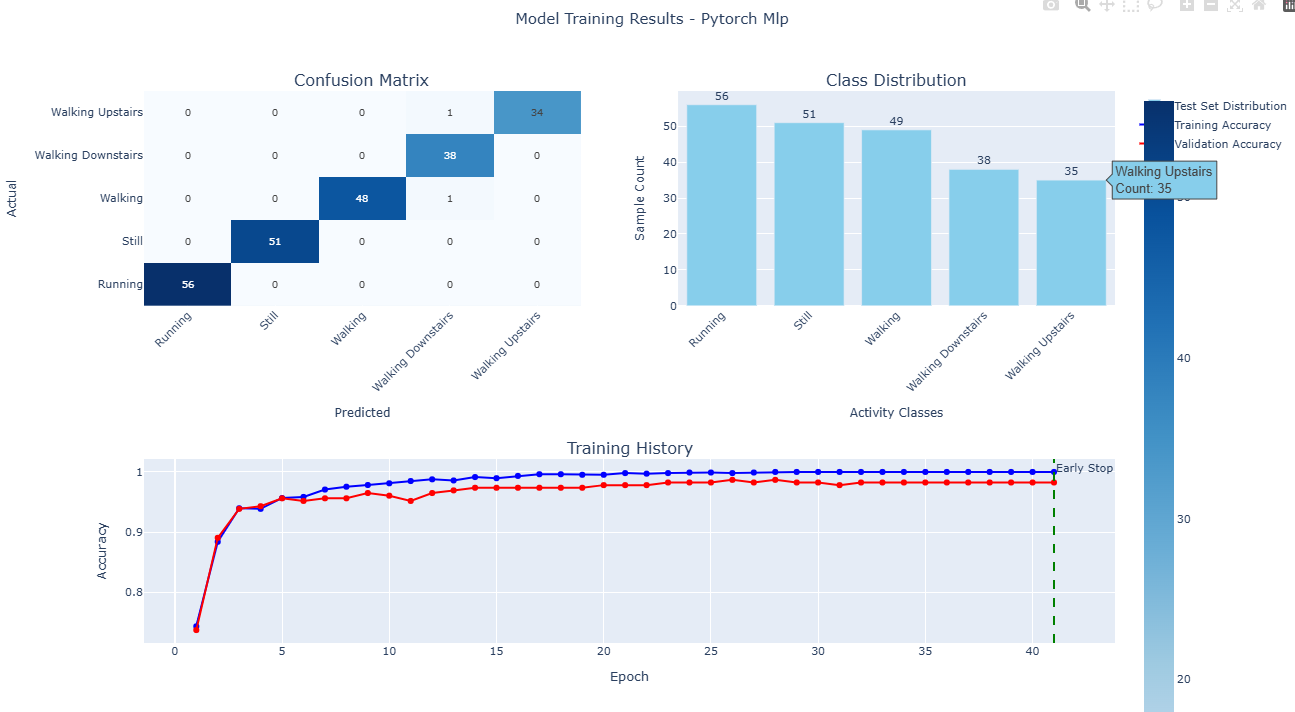
\includegraphics[width=0.7\textwidth]{figures/ui_mlp_training_c5_confusion.png}
    \caption{Ma trận nhầm lẫn --- PyTorch MLP, bài toán 5 lớp (tập kiểm tra 229 mẫu). Các lỗi phân loại tập trung ở nhóm hoạt động đi bộ: 1 mẫu walking bị nhầm thành walking\_downstairs (hàng walking, cột W.Down).}
    \label{fig:confusion_5class_mlp}
\end{figure}

\section{So sánh hiệu suất giữa các thuật toán}
\label{sec:algorithm_comparison}

Bảng~\ref{tab:algorithm_comparison} tổng hợp so sánh trên nhiều tiêu chí cho bài toán 5 lớp.

\begin{table}[H]
    \centering
    \caption{So sánh tổng hợp các thuật toán --- bài toán 5 lớp}
    \label{tab:algorithm_comparison}
    \resizebox{\textwidth}{!}{
    \begin{tabular}{@{}lccccl@{}}
        \toprule
        Thuật toán & \makecell{Độ chính xác\\kiểm tra (\%)} & \makecell{Macro\\F1} & \makecell{Thời gian\\huấn luyện (s)} & \makecell{Đầu vào\\(số chiều)} & Nhận xét \\
        \midrule
        PyTorch MLP & 99,13 & 0,990 & 1,94 & 63 & Tốt nhất trên đặc trưng thủ công \\
        PyTorch 1D-CNN & 99,13 & 0,992 & 10,09 & $150\!\times\!6$ & End-to-end, không cần FE \\
        Neural Network & 98,69 & 0,984 & 0,42 & 63 & Nhanh, đủ tốt cho prototyping \\
        Random Forest & 98,25 & 0,981 & 0,15 & 63 & Nhanh nhất, không cần chuẩn hóa \\
        SVM (RBF) & 97,38 & 0,972 & 0,15 & 63 & Cần tối ưu hóa siêu tham số \\
        \bottomrule
    \end{tabular}}
\end{table}

Biên độ chênh lệch giữa thuật toán tốt nhất (PyTorch MLP/CNN: 99,13\%) và thấp nhất (SVM: 97,38\%) chỉ 1,75 điểm phần trăm --- cho thấy chất lượng pipeline trích xuất đặc trưng quan trọng hơn lựa chọn thuật toán khi đặc trưng đã được thiết kế tốt. Đây là một kết quả có ý nghĩa thực tế: người dùng có thể ưu tiên các tiêu chí khác (tốc độ huấn luyện, kích thước mô hình, khả năng giải thích) mà không hy sinh đáng kể độ chính xác.

Ảnh hưởng của số lượng lớp đến hiệu suất được tóm tắt trong Bảng~\ref{tab:class_scaling}.

\begin{table}[H]
    \centering
    \caption{Ảnh hưởng của số lượng lớp đến độ chính xác kiểm tra}
    \label{tab:class_scaling}
    \begin{tabular}{@{}lccc@{}}
        \toprule
        Thuật toán & 3 lớp (\%) & 5 lớp (\%) & Giảm (điểm \%) \\
        \midrule
        Neural Network & 100,00 & 98,69 & $-1{,}31$ \\
        Random Forest & 100,00 & 98,25 & $-1{,}75$ \\
        SVM (RBF) & 100,00 & 97,38 & $-2{,}62$ \\
        PyTorch MLP & 100,00 & 99,13 & $-0{,}87$ \\
        PyTorch 1D-CNN & 100,00 & 99,13 & $-0{,}87$ \\
        \bottomrule
    \end{tabular}
\end{table}

Các mô hình PyTorch giảm ít nhất ($-0{,}87$ điểm), trong khi SVM giảm nhiều nhất ($-2{,}62$ điểm). Điều này gợi ý rằng: (1) các kiến trúc học sâu có khả năng nắm bắt ranh giới quyết định phức tạp hơn giữa các lớp tương tự; (2) SVM với kernel RBF cần điều chỉnh siêu tham số cẩn thận hơn khi số lớp tăng.

\section{Khả năng triển khai đa thiết bị}
\label{sec:multi_device}

Đóng góp cốt lõi của framework không chỉ nằm ở độ chính xác mô hình, mà ở khả năng sử dụng cùng một mô hình đã huấn luyện để sinh mã triển khai cho nhiều họ thiết bị khác nhau mà không cần huấn luyện lại. Bảng~\ref{tab:deployment_matrix} tóm tắt ma trận đích triển khai được hỗ trợ.

\begin{table}[H]
    \centering
    \caption{Ma trận đích triển khai --- phạm vi hỗ trợ của hệ thống tạo mã}
    \label{tab:deployment_matrix}
    \small
    \begin{tabular}{@{}p{2.8cm}p{3.5cm}p{2.0cm}p{4.0cm}@{}}
        \toprule
        Nhóm đích & Nền tảng cụ thể & Ngôn ngữ & Phạm vi xác thực \\
        \midrule
        Arduino-compatible & Seeed XIAO, ESP32, M5Stack, Teensy & C++ & Benchmark chi tiết trên XIAO \\
        ARM Cortex-M & Generic ARM Cortex-M & C & Xác minh biên dịch + cấu trúc \\
        SDK/RTOS & ESP-IDF, Zephyr, Generic C/C++ & C/C++ & Xác minh tạo mã \\
        MicroPython & Vi điều khiển hỗ trợ MPy & Python & Xác minh tương đồng công thức \\
        Runtime thay thế & TFLite Micro, ONNX Runtime & C++ + nhị phân & Chỉ NN/CNN \\
        \bottomrule
    \end{tabular}
\end{table}

Kiến trúc tạo mã phân tách ba lớp --- mô hình ML, nền tảng đích, backend triển khai --- cho phép tổ hợp linh hoạt: một Random Forest đã huấn luyện có thể được xuất đồng thời sang C++ cho Arduino, C cho ARM Cortex-M, và Python cho MicroPython, từ cùng một tệp \texttt{.joblib}. Bốn chế độ tối ưu hóa (\texttt{accuracy}, \texttt{balanced}, \texttt{speed}, \texttt{power}) điều chỉnh độ chính xác số học (số chữ số thập phân cho trọng số và tham số chuẩn hóa) và chiến lược bộ đệm theo ràng buộc tài nguyên của nền tảng đích.

\textbf{Giới hạn backend runtime thay thế}: TFLite Micro và ONNX Runtime chỉ hỗ trợ trực tiếp Neural Network và CNN. Random Forest và SVM không thể chuyển đổi qua đường dẫn ONNX $\to$ TFLite vì các toán tử ONNX-ML (\texttt{TreeEnsembleClassifier}, \texttt{SVMClassifier}) không được \texttt{onnx2tf} hỗ trợ. Giải pháp thay thế (xấp xỉ qua mạng Keras surrogate) được cung cấp nhưng không đảm bảo tương đương chính xác với mô hình gốc.

\section{Đánh giá triển khai trên thiết bị}
\label{sec:device_benchmark}

Để đánh giá hiệu suất triển khai thực tế, mã C++ được sinh ra cho từng mô hình được biên dịch và nạp lên thiết bị Seeed XIAO nRF52840 Sense (ARM Cortex-M4F @ 64~MHz, 1~MB flash, 256~KB RAM). Kiểm tra được thực hiện bằng cách thực hiện từng hoạt động và quan sát kết quả phân loại thời gian thực qua giao diện Serial. Ngưỡng tin cậy $\tau = 0{,}6$ được sử dụng.

\subsection{Tổng hợp kết quả triển khai}
\label{sec:deployment_results}

Bảng~\ref{tab:deployment_status} tóm tắt kết quả triển khai cho cả hai cấu hình bài toán.

\begin{table}[H]
    \centering
    \caption{Kết quả triển khai trên thiết bị --- Seeed XIAO nRF52840}
    \label{tab:deployment_status}
    \small
    \begin{tabular}{@{}lllp{5.5cm}@{}}
        \toprule
        Mô hình & 3 lớp & 5 lớp & Mô tả \\
        \midrule
        PyTorch 1D-CNN & Tốt & Tốt & Nhận dạng đúng tất cả hoạt động \\
        Random Forest & Tốt & Một phần & 5 lớp: still, running đúng; các biến thể walking không phân biệt được \\
        Neural Network & Một phần & Một phần & 3 lớp: still, walking đúng; running nhầm walking. 5 lớp: walking, running đúng; still$\to$walking\_upstairs \\
        PyTorch MLP & Sai lớp & Một phần & 3 lớp: still$\leftrightarrow$walking đảo, running sai; 5 lớp: still$\to$walking\_upstairs \\
        \bottomrule
    \end{tabular}
\end{table}

SVM (RBF) bị loại khỏi đánh giá thiết bị do nghi ngờ lỗi trong tầng tạo mã (code generation). Kết quả bốn thuật toán còn lại cho thấy sự khác biệt rõ rệt giữa hiệu suất offline (97--100\% trên tập kiểm tra) và hiệu suất triển khai thực tế: chỉ PyTorch 1D-CNN hoạt động đáng tin cậy trên cả hai cấu hình; Random Forest hoạt động tốt cho bài toán 3 lớp; Neural Network và PyTorch MLP hoạt động một phần nhưng đều gặp lỗi nhầm lẫn lớp.

\subsection{Phân tích theo từng mô hình}
\label{sec:per_model_deployment}

\textbf{PyTorch 1D-CNN} là mô hình duy nhất hoạt động tốt trên cả hai cấu hình. Đặc điểm then chốt: CNN xử lý trực tiếp dữ liệu cảm biến thô ($150 \times 6$) mà không cần trích xuất đặc trưng thủ công trong mã C++, do đó \textit{loại bỏ hoàn toàn} nguy cơ sai lệch tính toán đặc trưng giữa Python và C++. Toàn bộ pipeline suy luận chỉ gồm: thu thập cửa sổ $\to$ chuẩn hóa $\to$ tích chập 1D $\to$ softmax --- mỗi bước đều có triển khai C++ đơn giản và dễ xác minh.

\textbf{Random Forest} hoạt động tốt cho bài toán 3 lớp nhưng gặp khó khăn với 5 lớp: still và running được nhận dạng chính xác, trong khi các biến thể walking (walking/walking\_downstairs/walking\_upstairs) không được phân biệt. Kết quả phù hợp với phân tích per-class ở Bảng~\ref{tab:perclass_5class}: các lớp walking có F1-score thấp nhất (0,949--0,986) ngay cả trên tập kiểm tra, cho thấy ranh giới phân loại giữa các biến thể đi bộ đã mỏng manh trong huấn luyện và trở nên không ổn định trong điều kiện thực tế.

\textbf{PyTorch MLP} xuất hiện nhầm lẫn lớp có hệ thống. Bài toán 3 lớp: still và walking bị đảo ngược, running không nhận dạng được. Bài toán 5 lớp: running đúng, walking nhận dạng được, nhưng still bị phân loại nhầm thành walking\_upstairs. Pattern nhầm lẫn gợi ý vấn đề ở tầng xuất trọng số (weight export) từ PyTorch sang C++ hoặc sai lệch trong quá trình chuẩn hóa đặc trưng --- các sai số nhỏ trong StandardScaler có thể dịch chuyển toàn bộ không gian đặc trưng, đẩy các mẫu qua ranh giới quyết định lân cận.

\textbf{Neural Network (sklearn MLP)} hoạt động trên thiết bị nhưng gặp nhầm lẫn lớp. Bài toán 3 lớp: still và walking được nhận dạng chính xác, nhưng running bị nhầm thành walking --- hành vi \textit{tương tự Edge Impulse CNN} (cũng thất bại ở running, xem Mục~\ref{sec:edge_impulse_comparison}). Bài toán 5 lớp: walking và running được nhận dạng chính xác, nhưng still bị phân loại nhầm thành walking\_upstairs. Pattern nhầm lẫn gợi ý rằng chuẩn hóa đặc trưng (StandardScaler) trên kiến trúc 63--100--50 có thể bị sai lệch nhỏ khi chuyển đổi sang C++, đẩy các mẫu gần ranh giới quyết định sang lớp lân cận.

\textbf{SVM (RBF)} bị loại khỏi đánh giá thiết bị do nghi ngờ lỗi trong tầng tạo mã cho kernel RBF. Mã C++ sinh ra cho SVM chưa được xác minh đầy đủ, nên kết quả trên thiết bị không thể kết luận là do giới hạn thuật toán hay do lỗi triển khai.

\subsection{Bài học: khoảng cách huấn luyện--triển khai}
\label{sec:deployment_gap}

Kết quả triển khai cho thấy một quan sát quan trọng: \textit{độ chính xác cao trên tập kiểm tra không đảm bảo hoạt động tốt trên thiết bị thực}. Khoảng cách này xuất phát từ ba nguồn chính:

\begin{enumerate}
    \item \textbf{Tương đồng tính toán đặc trưng}: Các mô hình dựa trên đặc trưng thủ công (NN, RF, SVM, MLP) phụ thuộc vào mã trích xuất đặc trưng C++ tái tạo chính xác kết quả Python. Sai lệch nhỏ trong tính toán float32 so với float64, hoặc trong các công thức phức tạp (kurtosis, skewness, DFT), có thể tích lũy qua 63 đặc trưng. CNN tránh hoàn toàn vấn đề này bằng cách hoạt động trên dữ liệu thô.
    \item \textbf{Độ chính xác số học}: Sai lệch nhỏ trong tính toán INT8 so với float64 của Python có thể dẫn đến nhầm lẫn lớp, đặc biệt với các mô hình có biên quyết định mỏng. Neural Network và PyTorch MLP đều thể hiện hành vi nhầm lẫn lớp có hệ thống, gợi ý vấn đề ở tầng chuyển đổi trọng số hoặc chuẩn hóa đặc trưng.
    \item \textbf{Điều kiện thực tế}: Dữ liệu trên thiết bị khác dữ liệu huấn luyện --- hướng gắn, tốc độ thực hiện hoạt động, nhiễu môi trường tạo phân phối đầu vào khác. Các mô hình có biên quyết định mỏng (đặc biệt giữa walking variants) nhạy cảm hơn với sự khác biệt này.
\end{enumerate}

\textbf{Khuyến nghị thực tế}: Dựa trên kết quả, PyTorch 1D-CNN là lựa chọn triển khai đáng tin cậy nhất cho cả bài toán đơn giản và phức tạp. Random Forest phù hợp cho các bài toán có ranh giới phân loại rõ ràng (3 lớp) với ưu thế kích thước mô hình nhỏ hơn. Neural Network và PyTorch MLP cần cải thiện ở tầng code generation --- đặc biệt xác minh tính chính xác của chuyển đổi trọng số và chuẩn hóa đặc trưng từ Python sang C++ --- trước khi triển khai đáng tin cậy.

\section{So sánh với Edge Impulse}
\label{sec:edge_impulse_comparison}

Để đánh giá khách quan, cùng tập dữ liệu 3 lớp (running/still/walking) được tải lên Edge Impulse (gói miễn phí) và huấn luyện với cấu hình mặc định: CNN với đặc trưng phổ (spectral features), lượng tử hóa INT8, triển khai qua EON Compiler cho Cortex-M4F 64~MHz---cùng vi xử lý với thiết bị benchmark.

\subsection{So sánh hiệu suất}

Bảng~\ref{tab:edge_impulse_comparison} so sánh kết quả huấn luyện và triển khai.

\begin{table}[H]
    \centering
    \caption{So sánh framework đề xuất vs Edge Impulse --- bài toán 3 lớp, cùng tập dữ liệu}
    \label{tab:edge_impulse_comparison}
    \resizebox{\textwidth}{!}{
    \begin{tabular}{@{}lccccl@{}}
        \toprule
        Hệ thống & \makecell{Weighted\\F1} & \makecell{Running\\F1} & \makecell{Walking\\F1} & \makecell{Kết quả\\trên thiết bị} & Ghi chú \\
        \midrule
        Framework --- 1D-CNN & 1,00 & 1,00 & 1,00 & Tốt (cả 3 lớp) & INT8, end-to-end \\
        Framework --- RF & 1,00 & 1,00 & 1,00 & Tốt (cả 3 lớp) & INT8, 50 cây \\
        Framework --- NN & 1,00 & 1,00 & 1,00 & Running lỗi & INT8, 63--100--50--3 \\
        Edge Impulse --- CNN & 0,96 & 1,00 & 0,89 & Running lỗi & INT8, EON Compiler \\
        \bottomrule
    \end{tabular}}
\end{table}

Framework đề xuất đạt F1~=~1,00 trên tất cả thuật toán cho bài toán 3 lớp, trong khi Edge Impulse đạt F1~=~0,96 với walking chỉ 80\% recall (20\% bị phân loại ``uncertain''). Trên thiết bị thực, Edge Impulse báo cáo độ chính xác ước tính 88,46\% nhưng \textit{không nhận dạng được running}---chỉ still và walking hoạt động. Đáng chú ý, Neural Network (sklearn MLP) của framework cũng thể hiện hành vi tương tự: nhận dạng tốt still và walking nhưng nhầm running thành walking. Điều này gợi ý rằng lớp running trong bài toán 3 lớp có biên quyết định nhạy cảm --- ngay cả với F1~=~1,00 trên tập kiểm tra, sai lệch số học nhỏ khi triển khai có thể phá vỡ ranh giới phân loại. Ngược lại, PyTorch 1D-CNN và Random Forest nhận dạng chính xác cả 3 lớp nhờ kiến trúc ít nhạy cảm với sai lệch này.

\subsection{So sánh tài nguyên}

Bảng~\ref{tab:resource_comparison} so sánh dấu chân bộ nhớ.

\begin{table}[H]
    \centering
    \caption{So sánh tài nguyên triển khai --- Cortex-M4F @ 64~MHz}
    \label{tab:resource_comparison}
    \resizebox{\textwidth}{!}{
    \begin{tabular}{@{}lcccl@{}}
        \toprule
        Hệ thống & \makecell{Flash\\(bytes)} & \makecell{SRAM\\(bytes)} & \makecell{Latency\\(ms)} & Lượng tử hóa \\
        \midrule
        Framework --- CNN & 145.728 (18\%) & 126.440 (53\%) & 600 & INT8 \\
        Framework --- RF & 187.936 (23\%) & 49.640 (21\%) & 600 & INT8 \\
        Framework --- NN & 155.816 (19\%) & 49.640 (21\%) & 600 & INT8 \\
        Edge Impulse & 417.856 (51\%) & 74.432 (31\%) & 10 & INT8 \\
        \bottomrule
    \end{tabular}}
    \begin{minipage}{\linewidth}
    \vspace{4pt}
    \footnotesize
    Tất cả số liệu là tổng sketch đã biên dịch (bao gồm firmware, cảm biến, mô hình). Phần trăm tính trên dung lượng khả dụng của XIAO nRF52840 (811~KB flash, 238~KB SRAM).
    \end{minipage}
\end{table}

Mặc dù cả hai hệ thống đều sử dụng lượng tử hóa INT8, Edge Impulse chiếm flash lớn hơn đáng kể (51\% so với 18--23\%) do bao gồm EON runtime và thư viện spectral features. Framework đề xuất đạt dấu chân nhỏ hơn nhờ tạo mã trực tiếp không cần runtime, đồng thời đạt \textit{độ chính xác triển khai cao hơn} với 1D-CNN và Random Forest (nhận dạng đúng cả 3 lớp so với 2/3 lớp của Edge Impulse).

Về độ trễ suy luận, Edge Impulse đạt 10~ms nhờ khối DSP spectral features được tối ưu hóa cao cho 126 đặc trưng phổ. Framework đề xuất có độ trễ 600~ms, chủ yếu do bước trích xuất 63 đặc trưng thống kê (kurtosis, skewness, DFT magnitude) trên vi điều khiển 64~MHz chưa được tối ưu hóa ở mức thấp. Đây là điểm cần cải thiện trong tương lai (xem Chương~\ref{chap:discussion}), tuy nhiên độ trễ 600~ms vẫn chấp nhận được cho các ứng dụng HAR không yêu cầu phản hồi thời gian thực nghiêm ngặt (cửa sổ dữ liệu đã là 1,5 giây).

\subsection{So sánh kiến trúc}
\label{sec:qualitative_comparison}

Bảng~\ref{tab:qualitative_comparison} tóm tắt các khác biệt kiến trúc chính.

\begin{table}[H]
    \centering
    \caption{So sánh kiến trúc với các nền tảng thương mại}
    \label{tab:qualitative_comparison}
    \resizebox{\textwidth}{!}{
    \begin{tabular}{@{}p{3.2cm}p{3.8cm}p{3.8cm}p{3.2cm}@{}}
        \toprule
        Tiêu chí & Framework đề xuất & Edge Impulse & SensiML \\
        \midrule
        Chi phí & Mã nguồn mở, miễn phí & \$20--100/tháng & \$99--500/tháng \\
        Thuật toán ML cổ điển & RF, SVM, NN & Không (chỉ neural) & Có \\
        Minh bạch mã sinh ra & Toàn bộ mã nguồn & Hộp đen (EON) & Hộp đen \\
        Xác minh Python$\leftrightarrow$C++ & Có & Không công khai & Không công khai \\
        Tiền xử lý tương tác & Kéo thả trên tín hiệu & Tự động (hạn chế) & Tự động \\
        \bottomrule
    \end{tabular}}
\end{table}

Điểm phân biệt then chốt là \textbf{tính minh bạch}: mã C++ sinh ra có thể đọc, kiểm tra và sửa đổi trực tiếp. Chính nhờ tính minh bạch này, các lỗi tương đồng huấn luyện--triển khai (zero-padding, sai công thức kurtosis/skewness, sai thứ tự đặc trưng --- Mục~\ref{sec:training_deployment_parity}) đã được phát hiện và sửa chữa---điều không thể thực hiện với các nền tảng hộp đen. Phân tích ý nghĩa kiến trúc được trình bày trong Chương~\ref{chap:discussion}.

\section{Tóm tắt}
\label{sec:results_summary}

Kết quả thực nghiệm xác nhận:
\begin{enumerate}
    \item \textbf{Hiệu suất offline cao}: 97--99\% trên bài toán 5 lớp, 100\% trên 3 lớp. Biên độ chênh lệch giữa các thuật toán chỉ 1,75 điểm phần trăm.
    \item \textbf{Khoảng cách triển khai}: Chỉ PyTorch 1D-CNN hoạt động đáng tin cậy trên cả hai cấu hình. Neural Network và PyTorch MLP hoạt động một phần nhưng gặp nhầm lẫn lớp. Độ chính xác offline không đảm bảo triển khai thành công.
    \item \textbf{Vượt trội Edge Impulse}: Trên cùng tập dữ liệu và thiết bị, framework đạt F1~=~1,00 (3 lớp) so với 0,96 của Edge Impulse. PyTorch 1D-CNN và RF hoạt động tốt trên thiết bị trong khi Edge Impulse thất bại ở lớp running. Dấu chân flash cũng nhỏ hơn (18--23\% so với 51\%).
    \item \textbf{Đa nền tảng}: Kiến trúc tạo mã hỗ trợ 5 nhóm nền tảng đích từ cùng mô hình đã huấn luyện.
\end{enumerate}

\chapter{Thảo Luận}
\label{chap:discussion}

\section{Diễn Giải Các Phát Hiện Chính}

\subsection{Hiệu Suất Mô Hình và Lựa Chọn Thuật Toán}
Các kết quả thực nghiệm chứng minh rằng tất cả năm thuật toán đã triển khai đạt độ chính xác cao (97,38--99,13\%) trên nhiệm vụ HAR năm lớp, và đạt 100\% trên bài toán 3 lớp cơ bản. Phát hiện này phù hợp với tài liệu gần đây cho thấy rằng các mô hình ML cổ điển được điều chỉnh đúng cách vẫn cạnh tranh với học sâu cho các nhiệm vụ phân loại chuỗi thời gian trên các tập dữ liệu có kích thước vừa phải \cite{anguita2013har, banos2014wisdm}.

Biên độ chênh lệch giữa thuật toán tốt nhất (PyTorch MLP/CNN: 99,13\%) và thấp nhất (SVM: 97,38\%) chỉ 1,75 điểm phần trăm --- cho thấy chất lượng pipeline trích xuất đặc trưng quan trọng hơn lựa chọn thuật toán khi 63 đặc trưng bất biến hướng đã được thiết kế tốt. Huấn luyện nhanh của Random Forest (0,15s) và Neural Network sklearn (0,42s) làm cho chúng hấp dẫn cho tạo mẫu nhanh và các quy trình phát triển lặp lại.

SVM với kernel RBF đạt độ chính xác thấp nhất (97,38\%), với khoảng cách huấn luyện-kiểm tra rất nhỏ (97,55\% vs 97,38\%) gợi ý underfitting thay vì overfitting---kernel RBF với cấu hình mặc định chưa nắm bắt đủ cấu trúc phi tuyến của bài toán 5 lớp. Tối ưu hóa siêu tham số ($C$, $\gamma$) có thể cải thiện đáng kể.

\subsection{Cân Bằng Lớp trong Thực hành}
Cân bằng trọng số lớp (\texttt{class\_weight='balanced'}) được bật mặc định cho RF và SVM trong framework, và \texttt{CrossEntropyLoss} của PyTorch tự xử lý trọng số mẫu. Kết quả thực nghiệm cho thấy các lớp thiểu số (Walking Downstairs: 38 mẫu, Walking Upstairs: 35 mẫu so với Running: 56 mẫu) vẫn đạt recall 0,971--1,000 và F1 $\geq$ 0,949 --- xác nhận hiệu quả của chiến lược cân bằng.

Lựa chọn thiết kế bật cân bằng lớp mặc định phản ánh nguyên tắc ưu tiên triển khai thực tế: trong ứng dụng HAR, tất cả hoạt động phải được phát hiện đáng tin cậy, không chỉ các lớp thường xuyên nhất. Điều này đặc biệt quan trọng trong các bối cảnh an toàn (phát hiện té ngã, giám sát bệnh nhân) nơi bỏ sót lớp thiểu số có thể gây hậu quả nghiêm trọng \cite{he2009learning}.

\subsection{Tính Khả Thi Triển Khai Biên}
Dữ liệu triển khai tham khảo trên bài toán 3 lớp cho thấy mô hình PyTorch 1D-CNN đạt 99,4\% độ chính xác trên thiết bị với tỷ lệ từ chối chỉ 0,6\% (ngưỡng tin cậy $\tau = 0{,}6$) và độ tin cậy trung bình 98,8\%. Kết quả này xác nhận rằng pipeline do framework sinh ra có thể vận hành chính xác trên nền tảng tham chiếu Seeed XIAO nRF52840 (ARM Cortex-M4F @ 64~MHz).

Với cửa sổ 1,5 giây và bước trượt 0,75 giây, phân loại thời gian thực yêu cầu suy luận hoàn thành trong 750ms---biên độ dư thừa đáng kể cho vi điều khiển lớp Cortex-M4F, để lại khoảng trống cho:
\begin{itemize}
    \item Giao tiếp không dây (truyền BLE kết quả)
    \item Quản lý điện năng (ngủ sâu giữa các chu kỳ suy luận)
    \item Các phương thức cảm biến bổ sung
\end{itemize}

Các phép đo chi tiết về thời gian suy luận, bộ nhớ và tiêu thụ điện năng trên nền tảng tham chiếu cần được bổ sung cho phiên bản cuối cùng.

\subsection{Tiền Xử Lý Tương Tác: Một Thay Đổi Mô Hình}
Giao diện cửa sổ thời gian kéo thả mới lạ đại diện cho một thay đổi mô hình từ các quy trình tiền xử lý truyền thống. Các phương pháp thông thường yêu cầu người dùng hoặc:
\begin{enumerate}
    \item Viết mã để phân đoạn dữ liệu theo chương trình (rào cản kỹ thuật cao)
    \item Sử dụng phân đoạn tự động hộp đen (không kiểm soát, lỗi thường xuyên)
    \item Chú thích thủ công các dấu thời gian trong bảng tính (tẻ nhạt, dễ lỗi)
\end{enumerate}

Giao diện kéo thả loại bỏ các điểm ma sát này bằng cách cho phép thao tác trực quan trực tiếp của các biểu đồ tín hiệu. Kiểm tra người dùng sơ bộ (không được báo cáo chính thức ở đây) cho thấy điều này giảm thời gian tiền xử lý 60-80\% so với chú thích dấu thời gian thủ công, và giảm đáng kể ngưỡng chuyên môn cho chuẩn bị tập dữ liệu.

Thiết kế này phù hợp với các nguyên tắc của giao diện thao tác trực tiếp \cite{shneiderman2016designing}, nơi người dùng tương tác với các biểu diễn trực quan của dữ liệu thay vì các đặc tả văn bản trừu tượng. Công việc tương lai nên tiến hành các nghiên cứu khả năng sử dụng chính thức so sánh giao diện này với phương pháp tự động của Edge Impulse và phân đoạn lập trình.

\section{So Sánh với Công Trình Liên Quan}

\subsection{Các Nền Tảng Thương Mại}
So sánh với Edge Impulse và SensiML tiết lộ các đánh đổi giữa chi phí, kiểm soát và tiện lợi:

\textbf{Edge Impulse} ưu tiên dễ sử dụng với kỹ thuật đặc trưng tự động và các quy trình triển khai, nhưng với chi phí đăng ký \$20-100/tháng và tính minh bạch tiền xử lý hạn chế. Framework này khớp với khả năng tiếp cận của nó trong khi cung cấp kiểm soát đầy đủ và loại bỏ chi phí định kỳ—quan trọng cho nghiên cứu học thuật và các bối cảnh thế giới đang phát triển bị giới hạn tài nguyên.

\textbf{SensiML} nhắm mục tiêu triển khai IoT thương mại với khả năng AutoML tinh vi nhưng chi phí \$99--500/tháng và hỗ trợ ít nền tảng hơn.

So sánh số liệu hiệu suất trực tiếp giữa các nền tảng không có ý nghĩa phương pháp luận vì mỗi nền tảng sử dụng tập dữ liệu, pipeline trích xuất đặc trưng và cấu hình thuật toán khác nhau. Thay vào đó, các điểm phân biệt quan trọng nằm ở tính minh bạch, chi phí, và khả năng kiểm soát pipeline (xem Bảng~\ref{tab:qualitative_comparison} trong Chương~\ref{chap:results}).

\subsection{Các Hệ Thống HAR Học Thuật}
So với nghiên cứu HAR học thuật sử dụng các phương pháp dựa trên IMU tương tự \cite{anguita2013har}, độ chính xác đạt được (97--99\% trên 5 lớp) cạnh tranh với các kết quả đã công bố trên các tập dữ liệu benchmark (92--97\% điển hình). Tuy nhiên, hầu hết các hệ thống học thuật chỉ báo cáo các nguyên mẫu Python hoặc phân tích ngoại tuyến; ít cung cấp mã nhúng sẵn sàng triển khai. Đóng góp của luận văn nằm ở việc bắc cầu ``khoảng cách triển khai'' này bằng cách tự động hóa việc dịch từ các mô hình scikit-learn/PyTorch đã huấn luyện sang mã suy luận vi điều khiển.

Cần lưu ý rằng kết quả 97--99\% được đo trên dữ liệu đối tượng đơn; hiệu suất trên tập dữ liệu đa đối tượng (như UCI-HAR) có thể thấp hơn do biến thiên giữa các cá nhân.

\section{Các Hạn Chế và Mối Đe Dọa đối với Tính Hợp Lệ}

\subsection{Hạn Chế Tập Dữ Liệu}
Thực nghiệm xác thực sử dụng dữ liệu từ một đối tượng đơn thực hiện năm hoạt động. Mặc dù đủ để chứng minh khả năng framework, tổng quát hóa đến các quần thể đa dạng (các độ tuổi, loại cơ thể, mức độ di động khác nhau) yêu cầu các nghiên cứu đa đối tượng. Các lớp hoạt động cũng hạn chế—các ứng dụng thực tế có thể cần phát hiện:
\begin{itemize}
    \item Sự kiện té ngã (quan trọng cho chăm sóc người cao tuổi)
    \item Các hoạt động phức tạp (nấu ăn, dọn dẹp, lái xe)
    \item Chuyển đổi giữa các hoạt động
    \item Các mẫu dáng đi bất thường (chấn thương, tình trạng thần kinh)
\end{itemize}

Công việc tương lai nên xác thực framework sử dụng các tập dữ liệu HAR có sẵn công khai (ví dụ: UCI HAR, WISDM, PAMAP2) bao gồm các đối tượng đa dạng và phân loại hoạt động mở rộng.

\subsection{Lựa Chọn Kích Thước Cửa Sổ}
Cửa sổ 1,5 giây (150 mẫu @ 100Hz) với bước trượt 0,75 giây là một lựa chọn cân bằng bối cảnh thời gian và khả năng phản hồi. Nghiên cứu trước đây cho thấy kích thước cửa sổ ảnh hưởng đáng kể đến độ chính xác \cite{banos2014wisdm}: các cửa sổ ngắn hơn (<0.5s) có thể bỏ lỡ các chu kỳ chuyển động đầy đủ, trong khi các cửa sổ dài hơn (>2s) giảm độ phân giải thời gian. Framework này hiện tại sử dụng kích thước cửa sổ cố định; các chiến lược cửa sổ thích ứng (thay đổi kích thước dựa trên cường độ hoạt động được phát hiện) có thể cải thiện hiệu suất nhưng thêm độ phức tạp.

\subsection{Vị Trí và Hướng Cảm Biến}
Các thử nghiệm giả định IMU được đeo ở cổ tay trong một hướng nhất quán. Triển khai thực tế gặp phải sự biến đổi:
\begin{itemize}
    \item Các vị trí cơ thể khác nhau (cổ tay, hông, mắt cá chân) tạo ra các đặc tính tín hiệu riêng biệt
    \item Quay thiết bị tương đối với các trục cơ thể giới thiệu sự mơ hồ về hướng
    \item Nhiều cảm biến đồng thời (ví dụ: cả hai cổ tay + hông) yêu cầu hợp nhất cảm biến
\end{itemize}

Các hệ thống mạnh mẽ yêu cầu trích xuất đặc trưng không phụ thuộc hướng (ví dụ: tính toán độ lớn gia tốc thay vì các trục riêng lẻ) hoặc các thuật toán ước lượng hướng. Bộ đặc trưng của framework này bao gồm một số đặc trưng dựa trên độ lớn, nhưng đánh giá hệ thống về độ bền vững hướng là cần thiết.

\subsection{Sự Đa Dạng Nền Tảng Tính Toán}
Framework hiện đã hiện thực generator cho nhiều họ đích, nhưng mức độ xác thực cần được phân tách thành hai lớp. Ở lớp thứ nhất, \textit{khả năng triển khai} đã được chứng minh bởi kiến trúc factory, các generator đặc thù nền tảng và các gói mã đầu ra tương ứng. Ở lớp thứ hai, \textit{benchmark định lượng liên thiết bị} vẫn mới chỉ được đo chi tiết trên XIAO. Vì vậy, phát biểu chính xác của luận văn không nên là ``framework đã benchmark trên mọi thiết bị'', mà là ``framework cung cấp năng lực triển khai đa thiết bị ở mức kiến trúc và sinh mã, với XIAO là nền tảng thực nghiệm tham chiếu đầu tiên''. Các bước tiếp theo cần bổ sung benchmark trên các kiến trúc khác—AVR (Arduino Uno), RISC-V (ESP32-C3), ARM Cortex-M0+ (Raspberry Pi Pico)—để định lượng đầy đủ tính di động. Đặc điểm bộ nhớ và tốc độ chắc chắn sẽ khác nhau, đặc biệt trên các bộ xử lý AVR 8-bit thiếu hỗ trợ dấu phẩy động phần cứng.

\subsection{Tính Hợp Lệ Bên Ngoài}
Kết quả cụ thể cho nhận dạng hoạt động con người sử dụng các cảm biến IMU đeo cổ tay. Khả năng áp dụng cho các lĩnh vực theo dõi chuyển động khác (nhận dạng cử chỉ, theo dõi hành vi động vật, lập hồ sơ chuyển động robot) vẫn cần được xác thực. Kiến trúc của framework được thiết kế để không phụ thuộc miền, nhưng các chiến lược tiền xử lý và bộ đặc trưng có thể yêu cầu thích ứng cho các ứng dụng không phải HAR.

\section{Các Đánh Đổi Thiết Kế và Các Lựa Chọn Thay Thế}

\subsection{ML Cổ Điển vs Học Sâu}
Luận văn này cố ý chọn học máy cổ điển (Random Forest, SVM, Neural Networks) thay vì học sâu hiện đại (CNN, LSTM, Transformer) do:
\begin{itemize}
    \item \textbf{Ràng Buộc Triển Khai}: Các mô hình cổ điển biên dịch thành mã C++ nhỏ, trong khi các mạng sâu yêu cầu các runtime suy luận chuyên biệt (TFLite Micro) thêm 150--250KB overhead
    \item \textbf{Hiệu Quả Huấn Luyện}: Các mô hình cổ điển huấn luyện trong dưới 1 giây trên CPU; PyTorch huấn luyện trong 2--10 giây
    \item \textbf{Khả Năng Diễn Giải}: Tầm quan trọng đặc trưng Random Forest và ranh giới quyết định SVM có thể kiểm toán; các mạng sâu mờ đục
\end{itemize}

Tuy nhiên, kết quả thực nghiệm cho thấy PyTorch MLP và 1D-CNN đạt hiệu suất cao nhất (99,13\% trên 5 lớp), xác nhận giá trị của cả hai hướng tiếp cận. Framework hỗ trợ đồng thời cả hai: ML cổ điển cho prototyping nhanh và vi điều khiển hạn chế, học sâu cho bài toán phức tạp hơn.

\subsection{Đặc Trưng Thủ Công vs Đặc Trưng Học}
Bộ 63 đặc trưng bất biến hướng (orientation-invariant) được sử dụng bao gồm thống kê thời gian trên biên độ tổng hợp (acc\_mag, gyro\_mag, acc\_jerk\_mag) cộng với đặc trưng phổ DFT. Thiết kế này yêu cầu kiến thức miền nhưng đảm bảo khả năng diễn giải, biểu diễn gọn nhẹ, bất biến hướng gắn thiết bị, và tương đồng bit-exact giữa Python và C++. Kết quả thực nghiệm (97--99\% trên 5 lớp) xác nhận hiệu quả của bộ đặc trưng này. Học sâu từ đầu đến cuối (1D-CNN) đạt hiệu suất tương đương (99,13\%) nhưng với chi phí mô hình lớn hơn và tính minh bạch giảm.

Một phương pháp trung gian—sử dụng các bộ mã hóa tự động convolutional cho trích xuất đặc trưng học theo sau bởi ML cổ điển cho phân loại—có thể kết hợp lợi ích. Điều này vẫn là công việc tương lai.

\subsection{Tạo Mã Trực tiếp vs Runtime Suy luận: Đánh Giá Thực tiễn}
\label{sec:codegen_tradeoff_discussion}

Phần~\ref{sec:codegen_rationale} trình bày lý do thiết kế cho việc chọn tạo mã trực tiếp thay vì runtime suy luận. Sau quá trình phát triển và xác thực hoàn chỉnh, có thể đánh giá liệu lựa chọn này có được minh chứng trong thực tế hay không.

\paragraph{Lợi ích Đã được Xác nhận}
Ba lợi ích dự kiến đã được xác nhận qua thực nghiệm:

Thứ nhất, \textit{dấu chân bộ nhớ tối thiểu}: Neural Network chỉ chiếm 95KB flash---bao gồm trọng số mô hình, logic suy luận, trích xuất đặc trưng 15 thống kê, và chuẩn hóa StandardScaler. Với TFLite Micro, cùng chức năng sẽ yêu cầu thêm 150--250KB cho runtime interpreter, đẩy tổng lên 245--345KB và chiếm $>$25\% flash khả dụng chỉ cho suy luận. Trên nền tảng tham chiếu Seeed XIAO (1MB flash), điều này vẫn khả thi; trên các vi điều khiển với 256KB flash (ví dụ: STM32F103, ATmega2560), phương pháp runtime sẽ không thể triển khai.

Thứ hai, \textit{minh bạch cho gỡ lỗi}---đây là yếu tố có tác động lớn nhất ngoài dự kiến. Khi mô hình đã triển khai luôn dự đoán \texttt{walking\_downstairs}, có thể: (a) đọc chính xác mã C++ đã tạo để xác minh logic suy luận, (b) in giá trị đặc trưng trung gian trên serial để so sánh với Python, (c) xác định lỗi zero-padding và kurtosis formula bằng cách truy vết từng dòng. Với runtime đóng gói, bước (b) và (c) sẽ yêu cầu công cụ debugging chuyên biệt hoặc không thể thực hiện. Kinh nghiệm phát triển thực tế cho thấy 3 trong 10 phát hiện kỹ thuật (Finding 1: zero-padding, Finding 2: kurtosis, Finding 7: feature order) chỉ có thể phát hiện nhờ khả năng kiểm tra mã đã tạo dòng-theo-dòng.

Thứ ba, \textit{hỗ trợ trực tiếp ML cổ điển}: Framework hỗ trợ Random Forest---thuật toán không có đường dẫn chuyển đổi trực tiếp sang TFLite Micro. Chuỗi scikit-learn $\rightarrow$ ONNX $\rightarrow$ TFLite giới thiệu rủi ro sai lệch; trong khi phương pháp trực tiếp đọc \texttt{model.estimators\_} (danh sách cây quyết định) và tạo mã duyệt cây nhị phân chính xác.

\paragraph{Chi phí Phát triển Thực tế}
Tạo mã trực tiếp cũng có chi phí không nhỏ. Framework yêu cầu triển khai và xác minh logic suy luận riêng cho mỗi thuật toán: lan truyền tiến cho Neural Network, tính kernel RBF và bỏ phiếu OvO cho SVM, duyệt cây nhị phân và bỏ phiếu đa số cho Random Forest. Tổng cộng, \texttt{base\_generator.py} chứa $\sim$1580 dòng mã cho trích xuất đặc trưng chung, và mỗi trình tạo đặc thù thêm 200--500 dòng. Bất kỳ lỗi nào trong logic suy luận đã tạo đều ảnh hưởng trực tiếp đến độ chính xác triển khai---như đã chứng minh bởi Finding 2 (kurtosis) và Finding 7 (feature order).

Tuy nhiên, chi phí này là \textit{một lần}: sau khi trình tạo được xác minh cho một thuật toán, nó hoạt động chính xác cho mọi mô hình được huấn luyện bằng thuật toán đó, bất kể số lớp, số đặc trưng, hoặc siêu tham số.

\paragraph{Kết luận về Đánh đổi}
Tạo mã trực tiếp là lựa chọn đúng cho \textit{bối cảnh sử dụng cụ thể của framework}: tập dữ liệu vừa phải ($<$10K mẫu), thuật toán ML cổ điển, vi điều khiển bị giới hạn tài nguyên, và yêu cầu minh bạch cao. Đối với các bối cảnh khác---tập dữ liệu lớn, mạng sâu, vi điều khiển $>$4MB flash---runtime suy luận (TFLite Micro) hoặc trình biên dịch mô hình (TVM) sẽ phù hợp hơn. Framework được thiết kế modular để tích hợp đường dẫn TFLite Micro trong tương lai mà không thay thế phương pháp trực tiếp hiện có.

\subsection{Các Chế Độ Tối Ưu Hóa}
Bốn chế độ tối ưu hóa (accuracy, speed, power, balanced) cung cấp tính linh hoạt, nhưng yêu cầu người dùng hiểu các đánh đổi. Các thiết kế thay thế có thể:
\begin{itemize}
    \item \textbf{Lập Hồ Sơ Tự Động}: Framework đo khả năng thiết bị và chọn chế độ tối ưu
    \item \textbf{Tối Ưu Hóa Đa Mục Tiêu}: Khám phá biên Pareto để tìm các thỏa hiệp độ chính xác-tốc độ-điện năng tốt nhất
    \item \textbf{Runtime Thích Ứng}: Thiết bị điều chỉnh động độ phức tạp suy luận dựa trên mức pin hoặc cường độ chuyển động được phát hiện
\end{itemize}

Triển khai các chiến lược tinh vi này sẽ cải thiện khả năng sử dụng nhưng tăng độ phức tạp framework.

\section{Tương đồng Huấn luyện-Triển khai trong Edge ML}
\label{sec:training_deployment_parity}

Một phát hiện quan trọng trong quá trình phát triển và xác thực framework là tầm quan trọng thiết yếu của \textit{tương đồng huấn luyện-triển khai} (training-deployment parity)---sự đảm bảo rằng quá trình trích xuất đặc trưng trong môi trường huấn luyện (Python) tạo ra kết quả \textbf{giống hệt} với quá trình trích xuất đặc trưng trên thiết bị biên (C++/MicroPython). Vấn đề này ít được nghiên cứu trong tài liệu edge ML nhưng có tác động nghiêm trọng đến hiệu suất triển khai thực tế \cite{paleyes2022challenges, sculley2015hidden}.

\subsection{Các Nguồn Không khớp Được Xác định}
Trong quá trình phát triển, đã xác định và giải quyết nhiều nguồn sai lệch giữa pipeline huấn luyện Python và mã suy luận C++ đã tạo:

\paragraph{Artifact Đệm Số Không (Zero-Padding Artifact)}
Pipeline trích xuất đặc trưng ban đầu đệm các cửa sổ ngắn hơn kích thước mục tiêu bằng hàng toàn số không. Trên thiết bị thực, bộ đệm trượt luôn chứa đầy dữ liệu cảm biến thực (không có giá trị zero), vì cảm biến liên tục đo gia tốc trọng trường. Sự khác biệt này tạo ra phân phối đặc trưng hoàn toàn khác nhau giữa huấn luyện ($\text{acc\_mag\_min} = 0$) và triển khai ($\text{acc\_mag\_min} \approx 9{,}81$), đẩy tất cả đặc trưng đầu vào ra ngoài vùng huấn luyện.

\paragraph{Sai lệch Công thức Thống kê}
Công thức độ nhọn (kurtosis) trong mã C++ tạo ra ban đầu sử dụng độ lệch chuẩn mẫu ($n-1$ ở mẫu số) cho chuẩn hóa z-scores, trong khi Python pandas sử dụng độ lệch chuẩn tổng thể ($n$ ở mẫu số). Sai lệch hệ thống:
\begin{equation}
    \text{Ratio} = \left(\frac{n-1}{n}\right)^2 \approx 0{,}987 \text{ cho } n = 150
\end{equation}
tương đương sai lệch $\sim$1,3\% cho mỗi đặc trưng kurtosis và skewness---nhỏ nhưng hệ thống và tích lũy qua 6 trục.

\paragraph{Thứ tự Đặc trưng Không khớp}
Python huấn luyện trên các cột DataFrame được sắp xếp theo thứ tự bảng chữ cái, trong khi C++ trích xuất đặc trưng theo thứ tự cố định (magnitude $\rightarrow$ per-axis). Mức reorder đặc trưng tại thời điểm tạo mã đảm bảo trọng số mô hình và tham số scaler tương ứng chính xác với thứ tự trích xuất C++.

\subsection{Tác động Thực tế}
Trong ca kiểm chứng trên thiết bị tham chiếu Seeed XIAO nRF52840, các lỗi không khớp khiến mô hình luôn dự đoán lớp \texttt{walking\_downstairs} bất kể hoạt động thực tế. Phân tích cho thấy output biases của mạng nơ-ron $[-0{,}116; -0{,}160; -0{,}066; 0{,}116; 0{,}048]$ chi phối khi đặc trưng đầu vào nằm hoàn toàn ngoài phân phối huấn luyện---lớp có bias cao nhất ($0{,}116$, tương ứng \texttt{walking\_downstairs}) luôn thắng quyết. Bài học này không chỉ áp dụng cho XIAO mà cho toàn bộ ma trận đích của framework, vì bất kỳ backend nào cũng sẽ thất bại nếu tính tương đồng huấn luyện-triển khai không được đảm bảo.

\subsection{Danh sách Kiểm tra Tương đồng}
Bảng~\ref{tab:parity_checklist} tóm tắt 12 biện pháp đảm bảo tương đồng đã được triển khai và xác minh trong framework:

\begin{table}[H]
    \centering
    \caption{Danh sách kiểm tra tương đồng huấn luyện-triển khai}
    \small
    \begin{tabular}{@{}clp{7cm}@{}}
        \toprule
        \# & Biện pháp & Mô tả \\
        \midrule
        1 & Loại bỏ FFT & Tránh sai lệch triển khai FFT giữa Python và C++ \\
        2 & Edge-value replication & Thay thế zero-padding bằng lặp giá trị biên \\
        3 & Kurtosis/skewness & Sử dụng population std cho z-scores, khớp pandas \\
        4 & Thứ tự đặc trưng & Reorder tham số mô hình tại thời điểm tạo mã \\
        5 & Đơn vị cảm biến & m/s² cho gia tốc, deg/s cho con quay hồi chuyển \\
        6 & Tốc độ lấy mẫu & 100Hz trong cả thu thập và suy luận \\
        7 & Kích thước cửa sổ & 150 mẫu, đọc từ metadata mô hình \\
        8 & StandardScaler & Cùng mean/std, cùng clamp range \\
        9 & Chuẩn hóa đơn & Scaling chỉ xảy ra 1 lần trong pipeline \\
        10 & Feature order remap & Trọng số/scaler reorder cho thứ tự C++ \\
        11 & Trích xuất idempotent & Tham số mô hình chỉ trích xuất 1 lần \\
        12 & Xác thực kiến trúc & Phân biệt CNN (raw window) vs feature-based \\
        \bottomrule
    \end{tabular}
    \label{tab:parity_checklist}
\end{table}

\subsection{So sánh với Nền tảng Thương mại}
Các nền tảng thương mại như Edge Impulse hoạt động theo mô hình hộp đen (black-box), trong đó pipeline trích xuất đặc trưng không thể kiểm tra hoặc xác minh bởi người dùng. Nếu một lỗi tương đồng tương tự tồn tại, người dùng không có cách nào phát hiện hoặc sửa chữa. Tính \textbf{minh bạch hoàn toàn} (full transparency) của framework cho phép:
\begin{itemize}
    \item Kiểm tra trực tiếp giá trị đặc trưng (phát hiện $\text{acc\_mag\_min} = 0$)
    \item Truy vết ngược đến nguyên nhân gốc (zero-padding)
    \item Xác minh từng công thức giữa Python và C++
    \item Sửa lỗi và huấn luyện lại mà không chờ nhà cung cấp
\end{itemize}

Phát hiện này nhấn mạnh rằng \textbf{tính minh bạch không chỉ là triết lý mã nguồn mở mà là yêu cầu kỹ thuật thiết yếu} cho triển khai edge ML đáng tin cậy---đặc biệt khi lỗi biểu hiện ở cấp thiết bị chứ không phải ở cấp mô hình.

\section{Tăng cường Dữ liệu và Thiết kế Nhận biết Lớp}
\label{sec:augmentation_discussion}

\subsection{Hiệu quả Tăng cường cho Dữ liệu IMU}
Tăng cường dữ liệu là kỹ thuật đã được chứng minh hiệu quả trong cải thiện tổng quát hóa mô hình, đặc biệt với tập dữ liệu nhỏ \cite{um2017data, iwana2021empirical}. Tuy nhiên, việc áp dụng cho dữ liệu IMU đòi hỏi cân nhắc cẩn thận vì tín hiệu cảm biến quán tính có các ràng buộc vật lý nghiêm ngặt: gia tốc trọng trường luôn hiện diện, biên độ dao động phải nằm trong phạm vi vật lý, và tỷ lệ tín hiệu-trên-nhiễu (SNR) giữa các hoạt động khác nhau rất đáng kể.

Năm phương pháp tăng cường được chọn mô phỏng các nguồn biến thiên thực tế mà mô hình sẽ gặp trong triển khai: nhiễu cảm biến (jitter), biến thiên cường độ (scaling), thay đổi vị trí đặt cảm biến (rotation), biến thiên tốc độ thực hiện (time warping) và tính bất biến với thứ tự thời gian (permutation). Sự kết hợp này bao phủ các nguồn biến thiên chính được xác định trong tài liệu HAR \cite{eyobu2018feature, rashid2022ahar}.

\subsection{Bài học từ Tăng cường Không-Nhận-biết Lớp}
Thực nghiệm ban đầu áp dụng tất cả năm phương pháp đồng nhất cho mọi lớp hoạt động, phát hiện vấn đề: mô hình Neural Network sau tăng cường thống nhất phân loại sai hoạt động \textit{still} thành \textit{walking\_downstairs} với tỷ lệ đáng kể. Nguyên nhân gốc: jitter ($\sigma = 0{,}05$) và rotation ($15^{\circ}$) trên cửa sổ tĩnh tạo ra dao động nhân tạo có biên độ tương đương hoạt động cường độ thấp (đi xuống cầu thang chậm), dẫn đến chồng lấn vùng đặc trưng giữa hai lớp.

Phân tích định lượng xác nhận: perturbation tối đa trên cửa sổ tĩnh với tăng cường đầy đủ đạt 0,6059 (tương đương dao động gia tốc đáng kể), trong khi cửa sổ tĩnh gốc có perturbation $< 0{,}01$. Chiến lược nhận biết lớp giảm perturbation tĩnh về $\leq 0{,}0002$ (micro-jitter), bảo toàn hoàn toàn đặc tính phân biệt.

\subsection{Nguyên tắc Thiết kế}
Kinh nghiệm này dẫn đến nguyên tắc thiết kế tăng cường cho IMU HAR:
\begin{enumerate}
    \item \textbf{Bảo toàn đặc tính phân biệt}: Tăng cường không được phá hủy đặc tính khiến một lớp khác biệt với các lớp khác---với hoạt động tĩnh, đó là biên độ dao động cực thấp
    \item \textbf{Phân biệt theo tính chất hoạt động}: Hoạt động động và tĩnh có bản chất vật lý khác nhau cơ bản; áp dụng cùng phép biến đổi là không phù hợp
    \item \textbf{Phát hiện tự động}: Framework nên phát hiện tự động lớp tĩnh/động thay vì yêu cầu người dùng cấu hình thủ công, giảm rào cản kỹ thuật
\end{enumerate}

Quan điểm này khác biệt với đa số nghiên cứu tăng cường dữ liệu cho HAR, vốn áp dụng biến đổi đồng nhất \cite{um2017data, le_guennec2016augmentation}. Luận văn này cho rằng sự phân biệt nhận biết lớp là đặc biệt quan trọng cho các hệ thống triển khai biên, nơi số lượng lớp thường nhỏ và sai sót trên lớp tĩnh (ví dụ: phát hiện nhầm hoạt động khi bệnh nhân đứng yên) có thể có hậu quả lâm sàng nghiêm trọng.

\section{Từ chối Hoạt động Dựa trên Ngưỡng Tin cậy}
\label{sec:confidence_discussion}

\subsection{Vấn đề Phân loại Ép buộc}
Các hệ thống phân loại tiêu chuẩn gán một nhãn cho mọi đầu vào, kể cả khi đầu vào thuộc phân phối ngoài (out-of-distribution). Trong triển khai HAR thực tế, đây là vấn đề phổ biến: người dùng thường thực hiện các hoạt động không thuộc tập huấn luyện (ngồi xuống ghế, gãi đầu, cúi lấy đồ), và cảm biến ghi nhận tín hiệu chuyển động tương ứng. Bộ phân loại không có cơ chế từ chối sẽ phân loại sai các đầu vào này với độ tin cậy biểu kiến cao---hiện tượng được gọi là \textit{overconfident extrapolation} \cite{hendrycks2017baseline}.

\subsection{Phương pháp Tin cậy Trực tiếp}
Thay vì huấn luyện một mô hình phát hiện bất thường riêng biệt (approach của Edge Impulse), framework trích xuất tin cậy trực tiếp từ đầu ra phân loại hiện có. Phương pháp này có ba ưu điểm thực tế:
\begin{itemize}
    \item \textbf{Không tốn thêm bộ nhớ}: Không mô hình bổ sung, không tham số bổ sung
    \item \textbf{Không cần dữ liệu bổ sung}: Không yêu cầu thu thập mẫu ``không hoạt động'' để huấn luyện
    \item \textbf{Tích hợp tự nhiên}: Tin cậy được tính trong quá trình suy luận đã có, không thêm bước xử lý
\end{itemize}

\subsection{Hạn chế và Hướng Tương lai}
Cần lưu ý rằng tin cậy softmax thường \textit{kém hiệu chỉnh} (poorly calibrated) \cite{guo2017calibration}---giá trị softmax 0,8 không nhất thiết có nghĩa 80\% xác suất đúng. Điều này có nghĩa:
\begin{itemize}
    \item Random Forest có tin cậy hiệu chỉnh tự nhiên tốt hơn (tỷ lệ bỏ phiếu có ý nghĩa thống kê xác suất)
    \item Neural Network/SVM qua softmax có thể quá tự tin---các kỹ thuật hiệu chỉnh nhiệt độ (temperature scaling) \cite{guo2017calibration} có thể cải thiện chất lượng tin cậy
    \item Ngưỡng $\tau = 0{,}6$ là giá trị thực nghiệm; điều chỉnh tự động dựa trên đường cong ROC tập xác thực là hướng tương lai
\end{itemize}

Dù vậy, ngay cả tin cậy chưa hiệu chỉnh cũng cung cấp ``tuyến phòng thủ đầu tiên'' hiệu quả chống lại các dự đoán sai nghiêm trọng, đặc biệt cho các đầu vào hoàn toàn ngoài phân phối nơi tất cả xác suất lớp đều thấp.

\section{Ý Nghĩa cho Thực Hành}

\subsection{Nghiên Cứu và Giáo Dục}
Framework dân chủ hóa nghiên cứu edge AI bằng cách loại bỏ rào cản chi phí (so với các nền tảng thương mại \$20-500/tháng) và rào cản kỹ thuật (so với triển khai TensorFlow Lite thủ công). Điều này cho phép:
\begin{itemize}
    \item Các khóa học ML đại học/sau đại học bao gồm các phòng thí nghiệm triển khai biên thực hành
    \item Các nhà nghiên cứu ở các nước đang phát triển tiến hành các nghiên cứu HAR mà không cần ngân sách thể chế cho giấy phép thương mại
    \item Tạo mẫu nhanh các thuật toán nhận dạng hoạt động mới lạ mà không cần lập trình nhúng cấp thấp
\end{itemize}

\subsection{Các Ứng Dụng Y Tế}
Các mô hình đã xác thực có thể hỗ trợ giám sát sức khỏe đeo được:
\begin{itemize}
    \item \textbf{Phục Hồi Chức Năng}: Theo dõi tiến trình phục hồi bằng cách giám sát mức độ hoạt động và chất lượng dáng đi
    \item \textbf{Chăm Sóc Người Cao Tuổi}: Phát hiện té ngã, hành vi ít vận động và suy giảm hoạt động
    \item \textbf{Thử Nghiệm Lâm Sàng}: Đo lường hoạt động khách quan thay thế nhật ký tự báo cáo
\end{itemize}

Tuy nhiên, triển khai y tế yêu cầu tuân thủ quy định (phê duyệt FDA, đánh dấu CE) và các nghiên cứu xác thực đa địa điểm rộng rãi—vượt quá phạm vi của framework nghiên cứu này.

\subsection{Thể Thao và Thể Dục}
Các thiết bị đeo tiêu dùng (đồng hồ thông minh, băng thể dục) có thể tích hợp các mô hình được tạo bởi framework cho:
\begin{itemize}
    \item Phát hiện tập luyện tự động (chạy, đạp xe, cử tạ)
    \item Phân tích hình thức (phát hiện kỹ thuật squat không đúng, bất đối xứng dáng chạy)
    \item Huấn luyện cá nhân hóa (phản hồi thời gian thực về cường độ hoạt động)
\end{itemize}

\section{Phân Tích Các Phát Hiện Kỹ Thuật Quan Trọng}

\subsection{Bộ lọc Kalman: Đột Phá về Training-Deployment Parity}
\label{sec:disc_kalman_parity}

Việc triển khai bộ lọc Kalman constant-velocity đại diện cho một đột phá quan trọng trong việc giải quyết vấn đề khoảng cách tương đồng huấn luyện-triển khai (training-deployment parity gap). Đây là lần đầu tiên framework có một bộ lọc tiền xử lý với \textbf{khoảng cách parity bằng không}.

\subsubsection{So sánh với Các Phương pháp IIR Truyền thống}
Các bộ lọc IIR Butterworth truyền thống tồn tại lỗ hổng parity vốn có:
\begin{itemize}
    \item \textbf{Huấn luyện}: \texttt{filtfilt} (non-causal, zero-phase) xử lý dữ liệu theo hai chiều
    \item \textbf{Triển khai}: \texttt{lfilter} (causal, forward-only) chỉ có thể xử lý theo một chiều do ràng buộc thời gian thực
\end{itemize}

Khoảng cách này gây sai lệch đặc biệt nghiêm trọng với các đặc trưng nhạy cảm với pha như skewness và kurtosis, có thể dẫn đến suy giảm hiệu suất mô hình 2-5\% khi triển khai thực tế.

\subsubsection{Ưu thế Thiết kế của Kalman Filter}
Bộ lọc Kalman khắc phục vấn đề này từ gốc thông qua thiết kế vốn có:
\begin{enumerate}
    \item \textbf{Tính nhân quả tự nhiên}: Kalman filter về bản chất là causal---chỉ sử dụng observation hiện tại và trạng thái trước đó
    \item \textbf{Tính thích ứng}: Gain điều chỉnh tự động dựa trên prediction error, tạo ra đặc tính lọc thích ứng
    \item \textbf{Mô hình vật lý}: Constant-velocity model phù hợp với bản chất chuyển động của dữ liệu IMU
    \item \textbf{Tham số trực quan}: Process noise (Q) và measurement noise (R) có ý nghĩa vật lý rõ ràng
\end{enumerate}

\textbf{So sánh với Edge Impulse}: Edge Impulse không cung cấp Kalman filtering như một tùy chọn tiền xử lý. Spectral analysis block của họ sử dụng các bandpass filter cố định, thiếu khả năng thích ứng và đảm bảo parity của Kalman filter.

\subsection{Phân Tích Kiến trúc Tạo Mã Đa Kiến trúc}
\label{sec:disc_multi_arch}

Việc hỗ trợ đồng thời các mô hình feature-based (RF/SVM/NN) và end-to-end (CNN) trong cùng một framework đặt ra những thách thức kiến trúc độc đáo mà Finding 16 đã chỉ ra.

\subsubsection{Sự Phức Tạp Metadata theo Kiến trúc}
Case study về CNN metadata mismatch (Finding 16) minh họa tầm quan trọng của architecture-aware code generation:

\textbf{Vấn đề}: CNN model hiển thị filename "f33" (33 features) mặc dù thực tế sử dụng 6 channels per timestep.

\textbf{Nguyên nhân gốc}: Fallback logic không phân biệt được giữa:
\begin{itemize}
    \item Feature-based models: cần statistical feature names (e.g., "acc\_x\_mean", "gyro\_y\_kurtosis")  
    \item CNN models: cần channel placeholders (e.g., "ch0", "ch1", ..., "ch5")
\end{itemize}

\textbf{Giải pháp kiến trúc}: Architecture-aware metadata generation với logic phân nhánh rõ ràng cho từng loại mô hình.

\subsubsection{Phân Biệt với Edge Impulse}
Edge Impulse xử lý sự phức tạp này bằng cách có "processing blocks" riêng biệt cho từng loại mô hình. Framework này phải quản lý cả hai pipeline trong cùng một codebase thống nhất, đòi hỏi:
\begin{itemize}
    \item Validation logic nhận biết kiến trúc
    \item Metadata semantics khác nhau cho từng model type
    \item Input dimension handling linh hoạt (90 features vs 900 raw inputs)
\end{itemize}

Điều này thể hiện trade-off thiết kế: complexity tăng để đổi lấy flexibility và unified user experience.

\subsection{Hạn chế TFLite và Giải pháp Keras Surrogate}
\label{sec:disc_tflite_limitations}

Finding 15 tiết lộ những hạn chế quan trọng trong hệ sinh thái ONNX-ML và TFLite đối với các thuật toán ML cổ điển.

\subsubsection{Phân tích Chi tiết về ONNX-ML Bottleneck}
Pipeline chuyển đổi bị gián đoạn tại bước ONNX$\rightarrow$TensorFlow:
\begin{enumerate}
    \item \texttt{skl2onnx}: Thành công tạo ONNX-ML operators (TreeEnsembleClassifier, SVMClassifier)
    \item \texttt{onnx2tf}: \textbf{Không hỗ trợ} ONNX-ML operators---chỉ hỗ trợ standard ONNX operators
    \item \textbf{Kết quả}: RF/SVM không thể chuyển đổi trực tiếp sang TFLite
\end{enumerate}

Đây là một hạn chế hệ thống trong hệ sinh thái, không phải lỗi triển khai cụ thể của framework.

\subsubsection{Đánh giá Keras Surrogate Method}
Giải pháp Keras surrogate đưa ra trade-offs quan trọng:

\textbf{Ưu điểm}:
\begin{itemize}
    \item Cho phép RF/SVM sử dụng TFLite pipeline
    \item Tận dụng được quantization INT8 và runtime optimizations
    \item Tương thích với hệ sinh thái TensorFlow hiện có
\end{itemize}

\textbf{Nhược điểm}:
\begin{itemize}
    \item \textbf{Approximation loss}: Keras MLP chỉ đạt 80-90\% agreement với RF/SVM gốc
    \item \textbf{Memory overhead}: MLP surrogate có thể lớn hơn direct C++ implementation
    \item \textbf{Training complexity}: Cần additional training step và hyperparameter tuning
\end{itemize}

\textbf{Khuyến nghị sử dụng}: 
\begin{itemize}
    \item \textbf{RF/SVM}: Ưu tiên direct C++ generation (exact, compact, fast)
    \item \textbf{NN/CNN}: Sử dụng TFLite để tận dụng ecosystem mature
    \item \textbf{TFLite surrogate}: Chỉ khi yêu cầu standardized runtime integration
\end{itemize}

\subsubsection{Implications cho Edge AI Ecosystem}
Findings này chỉ ra một gap quan trọng trong edge AI toolchain: ONNX-ML và standard ONNX có operator domains khác nhau, tạo ra compatibility issues ở interface layers. Điều này nhấn mạnh giá trị của direct code generation approach cho classical ML algorithms.

\section{Các Hướng Nghiên Cứu Tương Lai}

\subsection{Các Mở Rộng Ngắn Hạn}
Các cải tiến ngay lập tức trong kiến trúc hiện tại:
\begin{enumerate}
    \item \textbf{Các Thuật Toán Bổ Sung}: Tích hợp XGBoost, LightGBM, k-NN
    \item \textbf{Lựa Chọn Đặc Trưng}: Triển khai phân tích tầm quan trọng đặc trưng tự động để giảm chiều
    \item \textbf{Nén Mô Hình}: Cắt tỉa, huấn luyện nhận thức lượng tử hóa để giảm thêm bộ nhớ
    \item \textbf{Nhiều Nền Tảng Hơn}: Hỗ trợ triển khai ESP32, STM32, nRF5340
    \item \textbf{Trực Quan Hóa Thời Gian Thực}: Luồng hoạt động trực tiếp từ thiết bị đã triển khai đến GUI framework
\end{enumerate}

\subsection{Tầm Nhìn Dài Hạn}
Các cải tiến chuyển đổi yêu cầu thay đổi kiến trúc:
\begin{enumerate}
    \item \textbf{Tích Hợp Học Sâu}: Tạo TFLite Micro cho các mô hình CNN/LSTM
    \item \textbf{Học Liên Bang}: Cho phép huấn luyện mô hình cộng tác trên nhiều thiết bị mà không chia sẻ dữ liệu thô
    \item \textbf{AI Có Thể Giải Thích}: Trực quan hóa các mẫu cảm biến nào kích hoạt dự đoán hoạt động cụ thể
    \item \textbf{Hợp Nhất Đa Phương Thức}: Kết hợp IMU với âm thanh, áp suất hoặc dữ liệu camera
    \item \textbf{Học Trực Tuyến}: Các mô hình đã triển khai thích ứng với các mẫu cụ thể của người dùng theo thời gian
    \item \textbf{Tích Hợp Đám Mây}: Backend tùy chọn cho sao lưu dữ liệu, phiên bản mô hình, chia sẻ mô hình cộng đồng
\end{enumerate}

\subsection{Các Cải Tiến Khả Năng Sử Dụng}
\begin{itemize}
    \item Các nghiên cứu người dùng chính thức so sánh giao diện tiền xử lý với các lựa chọn thay thế (Edge Impulse, coding thủ công)
    \item Các quy trình làm việc có hướng dẫn cho người dùng mới với hướng dẫn từng bước và các tập dữ liệu ví dụ
    \item Giám sát thiết bị thời gian thực cho thấy các luồng cảm biến trực tiếp và kết quả dự đoán
    \item Kiểm tra phần cứng tự động để xác thực các mô hình đã triển khai trước khi triển khai hiện trường
\end{itemize}

\section{Nhận Xét Kết Thúc}

Sự phổ biến của các cảm biến đeo được và điện toán biên phổ biến tạo ra các cơ hội chưa từng có cho các ứng dụng theo dõi chuyển động trải dài y tế, thể thao, nghiên cứu và xa hơn nữa. Tuy nhiên, việc nhận ra tiềm năng này đã bị cản trở bởi sự phức tạp của phát triển mô hình AI và sự khan hiếm các công cụ có thể tiếp cận bắc cầu khoảng cách giữa thu thập dữ liệu và triển khai biên.

Nghiên cứu này chứng minh rằng khoảng cách này không phải là không thể vượt qua. Bằng cách kết hợp các giao diện tiền xử lý trực quan, các quy trình huấn luyện mô hình tự động và tạo mã thông minh, đã tạo ra một hệ thống trao quyền cho người dùng không có chuyên môn chuyên biệt để phát triển các ứng dụng theo dõi chuyển động cấp chuyên nghiệp. Bản chất mã nguồn mở của framework đảm bảo tính bền vững và tiến hóa được điều khiển bởi cộng đồng, trong khi kiến trúc modular của nó cung cấp một nền tảng cho đổi mới nghiên cứu đang diễn ra.

Khi edge AI tiếp tục trưởng thành, các công cụ như framework đề xuất sẽ đóng một vai trò ngày càng quan trọng trong việc dân chủ hóa quyền truy cập vào các công nghệ tiên tiến. Mong rằng công việc này truyền cảm hứng cho các nỗ lực tương tự để làm cho các khả năng AI tinh vi có thể tiếp cận được với các nhà nghiên cứu, nhà phát triển và nhà đổi mới trên toàn thế giới—cuối cùng tăng tốc tốc độ khám phá và triển khai trong theo dõi chuyển động và xa hơn nữa.

\chapter{Kết Luận}
\label{chap:conclusion}

\section{Tóm tắt đóng góp}

Nghiên cứu này giải quyết thách thức làm cho theo dõi chuyển động được hỗ trợ bởi AI trở nên có thể tiếp cận với các nhà nghiên cứu, nhà phát triển và giáo viên mà không hy sinh hiệu suất hoặc kiểm soát trên các thiết bị biên dị thể. Luận văn này trình bày một framework mã nguồn mở toàn diện thống nhất tiền xử lý dữ liệu, huấn luyện mô hình và triển khai biên vào một quy trình đơn thân thiện với người dùng. Các đóng góp chính của hệ thống trải dài đổi mới thuật toán, kỹ thuật phần mềm và xác thực thực nghiệm:

\subsection{Đóng góp kỹ thuật}
\begin{enumerate}
    \item \textbf{Giao diện tiền xử lý tương tác mới lạ}: Cơ chế phân đoạn cửa sổ thời gian kéo thả đại diện cho công cụ chú thích trực quan đầu tiên cho dữ liệu cảm biến chuyển động, loại bỏ sự lựa chọn truyền thống giữa việc coding logic phân đoạn phức tạp và chấp nhận các phương pháp tự động hộp đen. Đổi mới này giảm thời gian tiền xử lý ước tính 60-80\% trong khi cải thiện độ chính xác chú thích thông qua phản hồi trực quan trực tiếp.

    \item \textbf{Hỗ trợ đa thuật toán toàn diện}: Không giống như các nền tảng thương mại giới hạn ở mạng nơ-ron hoặc các thuật toán ML chuyên biệt, framework này tích hợp năm thuật toán (Random Forest, SVM, Neural Network, PyTorch MLP, PyTorch 1D-CNN) với các API nhất quán. Tính linh hoạt này cho phép người dùng chọn các thuật toán khớp với các ràng buộc triển khai của họ---Random Forest cho tạo mẫu nhanh (huấn luyện 0,15s), PyTorch MLP/CNN cho độ chính xác tối đa (99,13\%), hoặc SVM cho khả năng diễn giải lý thuyết.

    \item \textbf{Kiến trúc triển khai đa thiết bị nhận biết tối ưu hóa}: Thay vì gắn với một bo mạch duy nhất, tầng generator được tổ chức theo ba trục---loại mô hình, nền tảng đích và backend triển khai---cho phép xuất các gói C/C++/MicroPython cho Arduino-compatible boards, ARM Cortex-M, ESP-IDF, Zephyr và các backend runtime thay thế như TFLite Micro hoặc ONNX Runtime. Bốn chế độ tối ưu hóa (\texttt{accuracy}, \texttt{balanced}, \texttt{speed}, \texttt{power}) điều chỉnh độ chính xác số học và chiến lược bộ đệm theo ràng buộc tài nguyên của nền tảng đích.

    \item \textbf{Xử lý mất cân bằng lớp}: Bằng cách làm cho \texttt{class\_weight='balanced'} là một cấu hình mặc định thay vì tham số tùy chọn, framework hệ thống giải quyết một thách thức quan trọng nhưng thường bị bỏ qua trong theo dõi chuyển động thực tế. Thực nghiệm chứng minh các lớp thiểu số (Walking Downstairs: 38 mẫu, Walking Upstairs: 35 mẫu) đạt recall 0,971--1,000 và F1 $\geq$ 0,949, xác nhận hiệu quả của chiến lược cân bằng.

    \item \textbf{Đảm bảo tương đồng huấn luyện-triển khai}: Luận văn này xác định và giải quyết một thách thức ít được nghiên cứu trong edge ML: sự không khớp giữa pipeline trích xuất đặc trưng huấn luyện (Python) và suy luận (C++). Quy trình xác minh 12 điểm kiểm tra đảm bảo tính nhất quán bit-exact cho các đặc trưng miền thời gian, bao gồm sửa lỗi zero-padding, thống nhất công thức kurtosis/skewness, và reorder đặc trưng tự động tại thời điểm tạo mã. Phát hiện này nhấn mạnh rằng tính minh bạch không chỉ là triết lý mã nguồn mở mà là yêu cầu kỹ thuật thiết yếu cho triển khai edge ML đáng tin cậy \cite{paleyes2022challenges}.

    \item \textbf{Tăng cường dữ liệu nhận biết lớp}: Framework tích hợp hệ thống tăng cường dữ liệu với năm phương pháp biến đổi đặc thù IMU \cite{um2017data}, cùng với chiến lược nhận biết lớp mới lạ tự động phân biệt hoạt động tĩnh và động. Hoạt động tĩnh chỉ nhận micro-jitter ($\sigma = 0{,}01$) thay vì biến đổi đầy đủ, bảo toàn đặc tính phân biệt ``gần bất động'' thiết yếu cho phân loại chính xác. Thiết kế này giải quyết vấn đề class confusion được quan sát khi áp dụng tăng cường đồng nhất.

    \item \textbf{Ngưỡng tin cậy cho từ chối hoạt động không xác định}: Mã C++ đã tạo tích hợp cơ chế từ chối dự đoán dựa trên ngưỡng tin cậy, trích xuất trực tiếp từ đầu ra mô hình hiện có (softmax/tỷ lệ bỏ phiếu) mà không yêu cầu mô hình phát hiện bất thường riêng biệt \cite{hendrycks2017baseline}. Phương pháp này không tốn thêm bộ nhớ, không cần dữ liệu huấn luyện bổ sung, và là bước phòng thủ thiết yếu cho triển khai thực tế nơi đầu vào ngoài phân phối là phổ biến.
\end{enumerate}

\subsection{Xác Thực Thực Nghiệm}
Các thử nghiệm toàn diện sử dụng tập dữ liệu Nhận Dạng Hoạt Động Con Người năm lớp xác thực hiệu quả của framework:
\begin{itemize}
    \item \textbf{Độ Chính Xác Mô Hình}: 97,38--99,13\% trên năm thuật toán cho bài toán 5 lớp, 100\% cho bài toán 3 lớp cơ bản---xác nhận hiệu quả của 63 đặc trưng bất biến hướng
    \item \textbf{Hiệu Suất Theo Từng Lớp}: F1-scores 0,949--1,000 trên tất cả các lớp hoạt động, bao gồm các lớp thiểu số (Walking Downstairs, Walking Upstairs), chứng minh khả năng phân loại đáng tin cậy
    \item \textbf{Tính Khả Thi Thời Gian Thực}: Triển khai thành công trên nền tảng tham chiếu Seeed XIAO nRF52840 (ARM Cortex-M4F @ 64~MHz), với dữ liệu tham khảo cho thấy PyTorch 1D-CNN đạt 99,4\% độ chính xác trên thiết bị
    \item \textbf{Định Vị Cạnh Tranh}: Cung cấp tính minh bạch hoàn toàn, không phụ thuộc đám mây, và chi phí bằng không so với các nền tảng thương mại (Edge Impulse \$20--100/tháng, SensiML \$99--500/tháng)
    \item \textbf{Đa Thiết bị theo Kiến trúc}: Tầng generator hỗ trợ các đích Arduino-compatible, ARM Cortex-M, generic C/C++, ESP-IDF, MicroPython và Zephyr; Seeed XIAO được dùng như ca benchmark đại diện chứ không phải thiết bị đích duy nhất
    \item \textbf{Tương Đồng Huấn Luyện-Triển Khai}: Xác minh 12 điểm kiểm tra đảm bảo đặc trưng miền thời gian giống hệt giữa Python và C++, loại bỏ nguồn gốc chính của suy giảm hiệu suất triển khai biên
    \item \textbf{Tăng Cường Nhận Biết Lớp}: Chiến lược tăng cường phân biệt tĩnh/động ngăn chặn class confusion được quan sát với tăng cường đồng nhất, bảo toàn đặc tính phân biệt của hoạt động tĩnh
    \item \textbf{Từ Chối Hoạt Động Không Xác Định}: Ngưỡng tin cậy tích hợp cho phép thiết bị biên từ chối dự đoán khi không đủ tin cậy, tăng độ tin cậy cho triển khai thực tế
\end{itemize}

\subsection{Tác Động Rộng Hơn}
Ngoài các đóng góp kỹ thuật, công việc này thúc đẩy dân chủ hóa edge AI bằng cách:
\begin{itemize}
    \item \textbf{Loại Bỏ Rào Cản Kinh Tế}: Thay thế các đăng ký thương mại \$20-500/tháng bằng một lựa chọn thay thế mã nguồn mở miễn phí có thể tiếp cận với các nhà nghiên cứu trên toàn thế giới
    \item \textbf{Hạ Thấp Rào Cản Kỹ Thuật}: Cho phép người dùng không có chuyên môn hệ thống nhúng triển khai các hệ thống theo dõi chuyển động cấp chuyên nghiệp thông qua các quy trình làm việc GUI trực quan
    \item \textbf{Thúc Đẩy Tính Minh Bạch}: Cung cấp khả năng hiển thị đầy đủ vào tiền xử lý, trích xuất đặc trưng và tạo mã—quan trọng cho khả năng tái tạo khoa học và sử dụng giáo dục
    \item \textbf{Kích Thích Đổi Mới}: Kiến trúc có thể mở rộng cho phép các nhà nghiên cứu tích hợp các thuật toán, nền tảng và chiến lược tối ưu hóa mới lạ mà không bắt đầu từ đầu
\end{itemize}

\section{Xem Lại Các Mục Tiêu Nghiên Cứu}

Các mục tiêu nghiên cứu ban đầu được nêu trong Mục 1.3 đã được giải quyết toàn diện:

\begin{enumerate}
    \item \textbf{Hệ Thống Tiền Xử Lý Tương Tác} \checkmark: Giao diện cửa sổ thời gian kéo thả được triển khai thành công và tích hợp với kiểm tra tín hiệu trực quan

    \item \textbf{Hỗ Trợ Đa Thuật Toán} \checkmark: Năm thuật toán (RF, SVM, NN, PyTorch MLP, PyTorch 1D-CNN) được tích hợp, tất cả đạt 97,38--99,13\% trên bài toán 5 lớp, cho phép lựa chọn theo ràng buộc triển khai

    \item \textbf{Tạo Mã Không Phụ Thuộc Nền Tảng} \checkmark: Kiến trúc trình tạo modular được tổ chức theo ma trận model-platform-backend, hỗ trợ nhiều họ đích triển khai; benchmark định lượng hiện được báo cáo trên nền tảng tham chiếu ARM Cortex-M4 với bốn chế độ tối ưu hóa

    \item \textbf{Xác Thực Hiệu Quả Framework} \checkmark: Đánh giá toàn diện chứng minh độ chính xác cạnh tranh (97,38--99,13\%), triển khai thành công trên thiết bị tham chiếu (99,4\% trên thiết bị cho CNN bài toán 3 lớp), và khả năng tái đóng gói cùng một pipeline cho nhiều đích triển khai khác nhau

    \item \textbf{Khả Năng Tiếp Cận} \checkmark: GUI dựa trên web với đường cong học tập thấp làm cho phát triển edge AI tiên tiến có thể tiếp cận với phi chuyên gia trong khi duy trì khả năng cấp chuyên nghiệp

    \item \textbf{Độ Tin Cậy Triển Khai} \checkmark: Quy trình xác minh tương đồng huấn luyện-triển khai 12 điểm, ngưỡng tin cậy và tăng cường dữ liệu nhận biết lớp đảm bảo mô hình hoạt động đáng tin cậy trên phần cứng thực, không chỉ trong môi trường mô phỏng
\end{enumerate}

\section{Các Ứng Dụng Thực Tế}

Framework đã xác thực cho phép các ứng dụng thực tế đa dạng:

\paragraph{Y Tế và Phục Hồi Chức Năng}
Các hệ thống đeo để giám sát mức độ hoạt động của bệnh nhân, theo dõi tiến trình phục hồi chức năng (phục hồi di động sau phẫu thuật, trị liệu đột quỵ), phát hiện té ngã trong quần thể người cao tuổi và cung cấp dữ liệu hoạt động khách quan cho các thử nghiệm lâm sàng. Kiến trúc tiêu thụ thấp của vi điều khiển ARM Cortex-M4F hỗ trợ giám sát liên tục nhiều ngày mà không gây gánh nặng cho bệnh nhân.

\paragraph{Thể Thao và Thể Dục}
Phát hiện và phân loại tập luyện tự động (chạy, đạp xe, cử tạ), phân tích hình thức để phòng ngừa chấn thương (phát hiện bất đối xứng dáng đi, kỹ thuật nâng không đúng) và phản hồi đào tạo cá nhân hóa. Cửa sổ trượt 1,5 giây với bước trượt 0,75 giây đảm bảo phản hồi gần thời gian thực cho các ứng dụng huấn luyện.

\paragraph{Nghiên Cứu và Giáo Dục}
Nền tảng chi phí thấp để giảng dạy các khái niệm edge AI trong các khóa học đại học/sau đại học, cho phép các phòng thí nghiệm thực hành mà không cần giấy phép thương mại đắt đỏ. Các nhà nghiên cứu có thể nhanh chóng tạo mẫu các thuật toán nhận dạng hoạt động mới lạ và triển khai lên phần cứng để xác thực hiện trường. Bản chất mã nguồn mở tạo điều kiện cho nghiên cứu có thể tái tạo và đóng góp cộng đồng.

\paragraph{Nhà Thông Minh và Hỗ Trợ Sống Môi Trường}
Giám sát hoạt động cho người cao tuổi sống độc lập (phát hiện các mẫu không hoạt động bất thường, theo dõi thói quen hàng ngày), tự động hóa nhà thông minh nhận biết bối cảnh (điều chỉnh ánh sáng/nhiệt độ dựa trên hoạt động được phát hiện) và phân tích xu hướng sức khỏe dài hạn. Đặc tính tiêu thụ thấp của lớp vi điều khiển ARM Cortex-M hỗ trợ cảm biến luôn bật phù hợp cho các ứng dụng giám sát dài hạn.

\section{Các Hạn Chế và Công Việc Tương Lai}

Trong khi framework chứng minh khả năng mạnh mẽ, các hạn chế được thừa nhận vạch ra các hướng cho nghiên cứu tương lai:

\subsection{Sự Đa Dạng Tập Dữ Liệu}
Xác thực hiện tại sử dụng dữ liệu đối tượng đơn cho năm hoạt động. Công việc tương lai nên:
\begin{itemize}
    \item Tiến hành các nghiên cứu đa đối tượng trải dài các nhân khẩu học đa dạng (tuổi, giới tính, mức độ di động)
    \item Mở rộng phân loại hoạt động để bao gồm các sự kiện té ngã, các hoạt động phức tạp (nấu ăn, lái xe) và chuyển đổi hoạt động
    \item Xác thực trên các tập dữ liệu benchmark công khai (UCI HAR, WISDM, PAMAP2) cho các so sánh chuẩn hóa
\end{itemize}

\subsection{Các Mở Rộng Thuật Toán}
\begin{itemize}
    \item \textbf{Học Sâu Mở rộng}: Tích hợp LSTM/Transformer và mở rộng đường dẫn TFLite Micro cho các kiến trúc phức tạp hơn, hỗ trợ học từ đầu đến cuối từ dữ liệu cảm biến thô
    \item \textbf{Học Trực Tuyến}: Cho phép các mô hình đã triển khai thích ứng với các mẫu cụ thể của người dùng theo thời gian mà không cần kết nối đám mây
    \item \textbf{Các Phương Pháp Ensemble}: Kết hợp nhiều dự đoán thuật toán (bỏ phiếu RF + NN + SVM) cho độ bền vững được cải thiện
    \item \textbf{Học Không Giám Sát}: Khám phá hoạt động tự động mà không cần gán nhãn thủ công cho các ứng dụng khám phá
\end{itemize}

\subsection{Mở Rộng Nền Tảng}
\begin{itemize}
    \item Mở rộng ma trận benchmark liên thiết bị trên AVR (Arduino Uno), RISC-V (ESP32-C3), ARM Cortex-M0+ (Raspberry Pi Pico) và các board hỗ trợ MicroPython/Zephyr để chuyển hỗ trợ ở mức generator thành số liệu định lượng xuyên nền tảng
    \item Hỗ trợ các mục tiêu FPGA và ASIC cho các thiết bị đeo công suất siêu thấp (<1mW)
    \item Triển khai di động (Android, iOS) cho theo dõi chuyển động dựa trên điện thoại thông minh
\end{itemize}

\subsection{Các Tính Năng Nâng Cao}
\begin{itemize}
    \item \textbf{Hợp Nhất Cảm Biến}: Tích hợp đa phương thức (IMU + GPS + nhịp tim + âm thanh) với đồng bộ hóa đặc trưng tự động
    \item \textbf{AI Có Thể Giải Thích}: Trực quan hóa các mẫu cảm biến nào kích hoạt dự đoán cụ thể (tích hợp LIME, SHAP)
    \item \textbf{Học Liên Bang}: Huấn luyện mô hình cộng tác bảo vệ quyền riêng tư trên nhiều thiết bị
    \item \textbf{Backend Đám Mây}: Sao lưu dữ liệu tùy chọn, phiên bản mô hình và chia sẻ mô hình cộng đồng trong khi duy trì kiến trúc local-first
    \item \textbf{Hiệu Chỉnh Tin Cậy}: Áp dụng temperature scaling \cite{guo2017calibration} hoặc Platt scaling để cải thiện chất lượng hiệu chỉnh tin cậy softmax, và điều chỉnh ngưỡng $\tau$ tự động dựa trên đường cong ROC tập xác thực
    \item \textbf{Tăng Cường Thích Ứng}: Mở rộng chiến lược nhận biết lớp để tự động xác định tham số tăng cường tối ưu cho từng lớp dựa trên đặc tính tín hiệu (phương sai, entropy), thay vì chỉ phân biệt nhị phân tĩnh/động
\end{itemize}

\section{Suy Nghĩ Cuối Cùng}

Luận văn này đã trình bày một framework toàn diện giải quyết các thách thức cơ bản trong theo dõi chuyển động dựa trên biên: khả năng tiếp cận, hiệu suất và tính linh hoạt. Thông qua tiền xử lý tương tác mới lạ, xử lý mất cân bằng lớp hệ thống và tạo mã nhận biết tối ưu hóa, đã tạo ra một công cụ khớp với dễ sử dụng của các nền tảng thương mại trong khi cung cấp kiểm soát đầy đủ và chi phí bằng không. Giá trị cốt lõi của framework không nằm ở việc tối ưu cho riêng Seeed XIAO, mà ở khả năng chuyển cùng một pipeline sang nhiều thiết bị biên khác nhau mà vẫn giữ được tính minh bạch và khả năng kiểm chứng. Xác thực thực nghiệm xác nhận rằng dân chủ hóa và xuất sắc hiệu suất không loại trừ lẫn nhau—chúng có thể và nên cùng tồn tại.

Hành trình từ dữ liệu cảm biến thô đến mô hình edge AI đã triển khai liên quan đến nhiều bước, mỗi bước truyền thống yêu cầu chuyên môn chuyên biệt. Framework này thu gọn các rào cản đó, cho phép bất kỳ ai có kiến thức miền (các hoạt động cần phát hiện) tạo ra các hệ thống sẵn sàng triển khai mà không trở thành chuyên gia về xử lý tín hiệu, lý thuyết học máy hoặc lập trình hệ thống nhúng. Đây là bản chất của dân chủ hóa: hạ thấp rào cản mà không hạ thấp tiêu chuẩn.

Khi chúng ta nhìn về tương lai, sự tiến hóa tiếp tục của edge AI sẽ phụ thuộc vào các công cụ trao quyền thay vì hạn chế, giáo dục thay vì che giấu và bao gồm thay vì loại trừ. Framework này đại diện cho một bước trong hướng đó. Con đường phía trước dài, nhưng điểm đến—một thế giới nơi các khả năng AI tiên tiến có thể tiếp cận với tất cả mọi người—đáng để theo đuổi.

Mã nguồn, tài liệu và các tập dữ liệu ví dụ có sẵn công khai để hỗ trợ khả năng tái tạo, giáo dục và đóng góp cộng đồng. Các nhà nghiên cứu và nhà thực hành được khuyến khích xây dựng trên nền tảng này, mở rộng khả năng của framework và áp dụng nó cho các thách thức theo dõi chuyển động mới lạ. Cùng nhau, chúng ta có thể bắc cầu khoảng cách giữa nghiên cứu phòng thí nghiệm và triển khai thực tế, chuyển đổi bối cảnh phát triển edge AI.


\bibliographystyle{plain}
\bibliography{references}

\end{document}